\documentclass[pdflatex,sn-mathphys-num]{sn-jnl}

\usepackage{graphicx}
\usepackage{amsmath,amssymb}
\usepackage{booktabs}
\usepackage{rotating}
\usepackage{adjustbox}
\usepackage{algorithm}
\usepackage{algorithmicx}
\usepackage{algpseudocode}
\usepackage{tikz}
\usetikzlibrary{arrows.meta,positioning,calc,fit,decorations.pathreplacing}
\usepackage{url}
\setlength{\emergencystretch}{3em}
\raggedbottom

% Generated by scripts/make_tables.py from the evidence registry; do not edit by hand.
\makeatletter
\newcommand{\V}[1]{\@ifundefined{acv@#1}{\PackageError{numbers}{Undefined value #1}{}}{\@nameuse{acv@#1}}}
\newcommand{\CI}[1]{\@ifundefined{acc@#1}{\PackageError{numbers}{Undefined interval #1}{}}{\@nameuse{acc@#1}}}
\@namedef{acv@abl.cum.bt}{68.47}
\@namedef{acv@abl.cum.by}{67.70}
\@namedef{acv@abl.cum.oc}{66.07}
\@namedef{acv@abl.host.bt}{68.49}
\@namedef{acv@abl.host.by}{67.70}
\@namedef{acv@abl.host.kitoc}{36.27}
\@namedef{acv@abl.host.oc}{66.44}
\@namedef{acv@abl.native.bt}{68.49}
\@namedef{acv@abl.native.by}{67.70}
\@namedef{acv@abl.native.oc}{66.44}
\@namedef{acv@abl.passthrough.byte}{byte-identical}
\@namedef{acv@abl.passthrough.cells}{7}
\@namedef{acv@abl.passthrough.identical}{7}
\@namedef{acv@abl.passthrough.st}{yes}
\@namedef{acv@abl.v6.bt}{62.55}
\@namedef{acv@abl.v6.by}{56.41}
\@namedef{acv@abl.v6.kitoc}{40.20}
\@namedef{acv@abl.v6.oc}{45.72}
\@namedef{acv@abl.v7d.bt}{68.37}
\@namedef{acv@abl.v7d.by}{67.56}
\@namedef{acv@abl.v7d.kitoc}{41.13}
\@namedef{acv@abl.v7d.oc}{65.70}
\@namedef{acv@abl.v7e.bt}{68.47}
\@namedef{acv@abl.v7e.by}{67.70}
\@namedef{acv@abl.v7e.kitoc}{44.15}
\@namedef{acv@abl.v7e.oc}{66.47}
\@namedef{acv@abl.v7f.bt}{68.49}
\@namedef{acv@abl.v7f.by}{67.70}
\@namedef{acv@abl.v7f.kitoc}{44.17}
\@namedef{acv@abl.v7f.oc}{66.91}
\@namedef{acv@bot.cat.base.int}{9}
\@namedef{acv@bot.cat.base.off}{12}
\@namedef{acv@bot.cat.g1.int}{3}
\@namedef{acv@bot.cat.g1.off}{9}
\@namedef{acv@bot.pool.int.dFN}{+12,737}
\@namedef{acc@bot.pool.int.dFN}{[+3,260, +24,205]}
\@namedef{acv@bot.pool.int.dFN.wl}{14/7}
\@namedef{acv@bot.pool.int.dFP}{\ensuremath{-}43,855}
\@namedef{acc@bot.pool.int.dFP}{[\ensuremath{-}72,450, \ensuremath{-}19,043]}
\@namedef{acv@bot.pool.int.dFP.wl}{5/16}
\@namedef{acv@bot.pool.int.dHOTA}{+1.44}
\@namedef{acc@bot.pool.int.dHOTA}{[+0.21, +2.68]}
\@namedef{acv@bot.pool.int.dHOTA.wl}{16/5}
\@namedef{acv@bot.pool.int.dIDF1}{+1.89}
\@namedef{acc@bot.pool.int.dIDF1}{[\ensuremath{-}0.19, +3.88]}
\@namedef{acv@bot.pool.int.dIDF1.wl}{17/4}
\@namedef{acv@bot.pool.int.dIDS}{\ensuremath{-}414}
\@namedef{acc@bot.pool.int.dIDS}{[\ensuremath{-}624, \ensuremath{-}224]}
\@namedef{acv@bot.pool.int.dIDS.wl}{5/16}
\@namedef{acv@bot.pool.int.dMOTA}{+15.61}
\@namedef{acc@bot.pool.int.dMOTA}{[+7.15, +25.68]}
\@namedef{acv@bot.pool.int.dMOTA.wl}{18/3}
\@namedef{acv@bot.pool.off.dFN}{+10,901}
\@namedef{acc@bot.pool.off.dFN}{[+2,914, +20,505]}
\@namedef{acv@bot.pool.off.dFN.wl}{15/6}
\@namedef{acv@bot.pool.off.dFP}{\ensuremath{-}36,636}
\@namedef{acc@bot.pool.off.dFP}{[\ensuremath{-}60,525, \ensuremath{-}15,875]}
\@namedef{acv@bot.pool.off.dFP.wl}{5/16}
\@namedef{acv@bot.pool.off.dHOTA}{+1.65}
\@namedef{acc@bot.pool.off.dHOTA}{[+0.26, +3.12]}
\@namedef{acv@bot.pool.off.dHOTA.wl}{16/5}
\@namedef{acv@bot.pool.off.dIDF1}{+1.93}
\@namedef{acc@bot.pool.off.dIDF1}{[\ensuremath{-}0.38, +4.04]}
\@namedef{acv@bot.pool.off.dIDF1.wl}{17/4}
\@namedef{acv@bot.pool.off.dIDS}{\ensuremath{-}1,958}
\@namedef{acc@bot.pool.off.dIDS}{[\ensuremath{-}2,741, \ensuremath{-}1,192]}
\@namedef{acv@bot.pool.off.dIDS.wl}{1/20}
\@namedef{acv@bot.pool.off.dMOTA}{+12.85}
\@namedef{acc@bot.pool.off.dMOTA}{[+5.72, +21.76]}
\@namedef{acv@bot.pool.off.dMOTA.wl}{17/4}
\@namedef{acv@bot.retinanet.base.FN}{40,306}
\@namedef{acv@bot.retinanet.base.FP}{37,619}
\@namedef{acv@bot.retinanet.base.HOTA}{31.73}
\@namedef{acv@bot.retinanet.base.IDF1}{32.18}
\@namedef{acv@bot.retinanet.base.IDS}{537}
\@namedef{acv@bot.retinanet.base.MOTA}{\ensuremath{-}16.51}
\@namedef{acv@bot.retinanet.base.Precision}{41.8}
\@namedef{acv@bot.retinanet.base.Recall}{40.1}
\@namedef{acv@bot.retinanet.g1.FN}{40,327}
\@namedef{acv@bot.retinanet.g1.FP}{30,274}
\@namedef{acv@bot.retinanet.g1.HOTA}{34.67}
\@namedef{acv@bot.retinanet.g1.IDF1}{36.73}
\@namedef{acv@bot.retinanet.g1.IDS}{451}
\@namedef{acv@bot.retinanet.g1.MOTA}{\ensuremath{-}5.50}
\@namedef{acv@bot.retinanet.g1.Precision}{47.2}
\@namedef{acv@bot.retinanet.g1.Recall}{40.1}
\@namedef{acv@bot.retinanet.int.dFN}{+21}
\@namedef{acc@bot.retinanet.int.dFN}{[\ensuremath{-}1,565, +1,636]}
\@namedef{acv@bot.retinanet.int.dFN.wl}{5/2}
\@namedef{acv@bot.retinanet.int.dFP}{\ensuremath{-}7,345}
\@namedef{acc@bot.retinanet.int.dFP}{[\ensuremath{-}15,979, \ensuremath{-}140]}
\@namedef{acv@bot.retinanet.int.dFP.wl}{2/5}
\@namedef{acv@bot.retinanet.int.dHOTA}{+2.94}
\@namedef{acc@bot.retinanet.int.dHOTA}{[+1.28, +4.54]}
\@namedef{acv@bot.retinanet.int.dHOTA.wl}{6/1}
\@namedef{acv@bot.retinanet.int.dIDF1}{+4.55}
\@namedef{acc@bot.retinanet.int.dIDF1}{[+1.78, +6.82]}
\@namedef{acv@bot.retinanet.int.dIDF1.wl}{6/1}
\@namedef{acv@bot.retinanet.int.dIDS}{\ensuremath{-}86}
\@namedef{acc@bot.retinanet.int.dIDS}{[\ensuremath{-}182, \ensuremath{-}4]}
\@namedef{acv@bot.retinanet.int.dIDS.wl}{3/4}
\@namedef{acv@bot.retinanet.int.dMOTA}{+11.00}
\@namedef{acc@bot.retinanet.int.dMOTA}{[+1.78, +24.77]}
\@namedef{acv@bot.retinanet.int.dMOTA.wl}{6/1}
\@namedef{acv@bot.retinanet.off.dFN}{\ensuremath{-}53}
\@namedef{acc@bot.retinanet.off.dFN}{[\ensuremath{-}1,511, +1,515]}
\@namedef{acv@bot.retinanet.off.dFN.wl}{4/3}
\@namedef{acv@bot.retinanet.off.dFP}{\ensuremath{-}5,855}
\@namedef{acc@bot.retinanet.off.dFP}{[\ensuremath{-}12,924, +453]}
\@namedef{acv@bot.retinanet.off.dFP.wl}{2/5}
\@namedef{acv@bot.retinanet.off.dHOTA}{+4.22}
\@namedef{acc@bot.retinanet.off.dHOTA}{[+2.98, +5.30]}
\@namedef{acv@bot.retinanet.off.dHOTA.wl}{7/0}
\@namedef{acv@bot.retinanet.off.dIDF1}{+5.59}
\@namedef{acc@bot.retinanet.off.dIDF1}{[+3.63, +7.07]}
\@namedef{acv@bot.retinanet.off.dIDF1.wl}{7/0}
\@namedef{acv@bot.retinanet.off.dIDS}{\ensuremath{-}959}
\@namedef{acc@bot.retinanet.off.dIDS}{[\ensuremath{-}1,377, \ensuremath{-}510]}
\@namedef{acv@bot.retinanet.off.dIDS.wl}{0/7}
\@namedef{acv@bot.retinanet.off.dMOTA}{+9.56}
\@namedef{acc@bot.retinanet.off.dMOTA}{[+1.44, +19.79]}
\@namedef{acv@bot.retinanet.off.dMOTA.wl}{6/1}
\@namedef{acv@bot.rtdetr.base.FN}{24,310}
\@namedef{acv@bot.rtdetr.base.FP}{51,836}
\@namedef{acv@bot.rtdetr.base.HOTA}{41.41}
\@namedef{acv@bot.rtdetr.base.IDF1}{47.23}
\@namedef{acv@bot.rtdetr.base.IDS}{381}
\@namedef{acv@bot.rtdetr.base.MOTA}{\ensuremath{-}13.63}
\@namedef{acv@bot.rtdetr.base.Precision}{45.4}
\@namedef{acv@bot.rtdetr.base.Recall}{63.9}
\@namedef{acv@bot.rtdetr.g1.FN}{36,691}
\@namedef{acv@bot.rtdetr.g1.FP}{16,242}
\@namedef{acv@bot.rtdetr.g1.HOTA}{43.56}
\@namedef{acv@bot.rtdetr.g1.IDF1}{49.58}
\@namedef{acv@bot.rtdetr.g1.IDS}{107}
\@namedef{acv@bot.rtdetr.g1.MOTA}{21.24}
\@namedef{acv@bot.rtdetr.g1.Precision}{65.4}
\@namedef{acv@bot.rtdetr.g1.Recall}{45.5}
\@namedef{acv@bot.rtdetr.int.dFN}{+12,381}
\@namedef{acc@bot.rtdetr.int.dFN}{[+5,456, +19,659]}
\@namedef{acv@bot.rtdetr.int.dFN.wl}{6/1}
\@namedef{acv@bot.rtdetr.int.dFP}{\ensuremath{-}35,594}
\@namedef{acc@bot.rtdetr.int.dFP}{[\ensuremath{-}51,960, \ensuremath{-}19,379]}
\@namedef{acv@bot.rtdetr.int.dFP.wl}{0/7}
\@namedef{acv@bot.rtdetr.int.dHOTA}{+2.15}
\@namedef{acc@bot.rtdetr.int.dHOTA}{[+0.16, +4.50]}
\@namedef{acv@bot.rtdetr.int.dHOTA.wl}{5/2}
\@namedef{acv@bot.rtdetr.int.dIDF1}{+2.35}
\@namedef{acc@bot.rtdetr.int.dIDF1}{[\ensuremath{-}1.17, +5.90]}
\@namedef{acv@bot.rtdetr.int.dIDF1.wl}{5/2}
\@namedef{acv@bot.rtdetr.int.dIDS}{\ensuremath{-}274}
\@namedef{acc@bot.rtdetr.int.dIDS}{[\ensuremath{-}389, \ensuremath{-}156]}
\@namedef{acv@bot.rtdetr.int.dIDS.wl}{0/7}
\@namedef{acv@bot.rtdetr.int.dMOTA}{+34.88}
\@namedef{acc@bot.rtdetr.int.dMOTA}{[+17.88, +52.96]}
\@namedef{acv@bot.rtdetr.int.dMOTA.wl}{7/0}
\@namedef{acv@bot.rtdetr.off.dFN}{+10,440}
\@namedef{acc@bot.rtdetr.off.dFN}{[+4,719, +16,494]}
\@namedef{acv@bot.rtdetr.off.dFN.wl}{7/0}
\@namedef{acv@bot.rtdetr.off.dFP}{\ensuremath{-}30,027}
\@namedef{acc@bot.rtdetr.off.dFP}{[\ensuremath{-}43,821, \ensuremath{-}16,964]}
\@namedef{acv@bot.rtdetr.off.dFP.wl}{0/7}
\@namedef{acv@bot.rtdetr.off.dHOTA}{+1.31}
\@namedef{acc@bot.rtdetr.off.dHOTA}{[\ensuremath{-}0.50, +3.55]}
\@namedef{acv@bot.rtdetr.off.dHOTA.wl}{4/3}
\@namedef{acv@bot.rtdetr.off.dIDF1}{+0.95}
\@namedef{acc@bot.rtdetr.off.dIDF1}{[\ensuremath{-}2.37, +4.47]}
\@namedef{acv@bot.rtdetr.off.dIDF1.wl}{4/3}
\@namedef{acv@bot.rtdetr.off.dIDS}{\ensuremath{-}930}
\@namedef{acc@bot.rtdetr.off.dIDS}{[\ensuremath{-}1,261, \ensuremath{-}559]}
\@namedef{acv@bot.rtdetr.off.dIDS.wl}{0/7}
\@namedef{acv@bot.rtdetr.off.dMOTA}{+28.56}
\@namedef{acc@bot.rtdetr.off.dMOTA}{[+13.77, +49.33]}
\@namedef{acv@bot.rtdetr.off.dMOTA.wl}{7/0}
\@namedef{acv@bot.yolov8.base.FN}{43,792}
\@namedef{acv@bot.yolov8.base.FP}{11,637}
\@namedef{acv@bot.yolov8.base.HOTA}{35.99}
\@namedef{acv@bot.yolov8.base.IDF1}{39.57}
\@namedef{acv@bot.yolov8.base.IDS}{226}
\@namedef{acv@bot.yolov8.base.MOTA}{17.36}
\@namedef{acv@bot.yolov8.base.Precision}{66.9}
\@namedef{acv@bot.yolov8.base.Recall}{35.0}
\@namedef{acv@bot.yolov8.g1.FN}{44,127}
\@namedef{acv@bot.yolov8.g1.FP}{10,721}
\@namedef{acv@bot.yolov8.g1.HOTA}{36.60}
\@namedef{acv@bot.yolov8.g1.IDF1}{40.40}
\@namedef{acv@bot.yolov8.g1.IDS}{172}
\@namedef{acv@bot.yolov8.g1.MOTA}{18.30}
\@namedef{acv@bot.yolov8.g1.Precision}{68.4}
\@namedef{acv@bot.yolov8.g1.Recall}{34.5}
\@namedef{acv@bot.yolov8.int.dFN}{+335}
\@namedef{acc@bot.yolov8.int.dFN}{[\ensuremath{-}1,373, +2,088]}
\@namedef{acv@bot.yolov8.int.dFN.wl}{3/4}
\@namedef{acv@bot.yolov8.int.dFP}{\ensuremath{-}916}
\@namedef{acc@bot.yolov8.int.dFP}{[\ensuremath{-}3,518, +1,421]}
\@namedef{acv@bot.yolov8.int.dFP.wl}{3/4}
\@namedef{acv@bot.yolov8.int.dHOTA}{+0.61}
\@namedef{acc@bot.yolov8.int.dHOTA}{[\ensuremath{-}0.05, +1.54]}
\@namedef{acv@bot.yolov8.int.dHOTA.wl}{5/2}
\@namedef{acv@bot.yolov8.int.dIDF1}{+0.83}
\@namedef{acc@bot.yolov8.int.dIDF1}{[\ensuremath{-}0.30, +2.21]}
\@namedef{acv@bot.yolov8.int.dIDF1.wl}{6/1}
\@namedef{acv@bot.yolov8.int.dIDS}{\ensuremath{-}54}
\@namedef{acc@bot.yolov8.int.dIDS}{[\ensuremath{-}93, \ensuremath{-}12]}
\@namedef{acv@bot.yolov8.int.dIDS.wl}{2/5}
\@namedef{acv@bot.yolov8.int.dMOTA}{+0.94}
\@namedef{acc@bot.yolov8.int.dMOTA}{[\ensuremath{-}1.03, +2.94]}
\@namedef{acv@bot.yolov8.int.dMOTA.wl}{5/2}
\@namedef{acv@bot.yolov8.off.dFN}{+514}
\@namedef{acc@bot.yolov8.off.dFN}{[\ensuremath{-}914, +2,051]}
\@namedef{acv@bot.yolov8.off.dFN.wl}{4/3}
\@namedef{acv@bot.yolov8.off.dFP}{\ensuremath{-}754}
\@namedef{acc@bot.yolov8.off.dFP}{[\ensuremath{-}3,527, +1,868]}
\@namedef{acv@bot.yolov8.off.dFP.wl}{3/4}
\@namedef{acv@bot.yolov8.off.dHOTA}{+0.34}
\@namedef{acc@bot.yolov8.off.dHOTA}{[\ensuremath{-}0.28, +1.15]}
\@namedef{acv@bot.yolov8.off.dHOTA.wl}{5/2}
\@namedef{acv@bot.yolov8.off.dIDF1}{+0.37}
\@namedef{acc@bot.yolov8.off.dIDF1}{[\ensuremath{-}0.75, +1.45]}
\@namedef{acv@bot.yolov8.off.dIDF1.wl}{6/1}
\@namedef{acv@bot.yolov8.off.dIDS}{\ensuremath{-}69}
\@namedef{acc@bot.yolov8.off.dIDS}{[\ensuremath{-}108, \ensuremath{-}29]}
\@namedef{acv@bot.yolov8.off.dIDS.wl}{1/6}
\@namedef{acv@bot.yolov8.off.dMOTA}{+0.43}
\@namedef{acc@bot.yolov8.off.dMOTA}{[\ensuremath{-}2.28, +2.77]}
\@namedef{acv@bot.yolov8.off.dMOTA.wl}{4/3}
\@namedef{acv@cal.bt.pow3.d}{+3.51}
\@namedef{acc@cal.bt.pow3.d}{[+0.85, +13.28]}
\@namedef{acv@cal.bt.pow3.native}{61.33}
\@namedef{acv@cal.bt.pow3.v7f}{64.84}
\@namedef{acv@cal.bt.pow3.verdict}{significant recovery}
\@namedef{acv@cal.bt.pow3.wtl}{7/0/0}
\@namedef{acv@cal.bt.temp2.d}{0.00}
\@namedef{acc@cal.bt.temp2.d}{[0.00, 0.00]}
\@namedef{acv@cal.bt.temp2.native}{67.59}
\@namedef{acv@cal.bt.temp2.v7f}{67.59}
\@namedef{acv@cal.bt.temp2.verdict}{identical output}
\@namedef{acv@cal.bt.temp2.wtl}{0/7/0}
\@namedef{acv@cal.byoff.pow3.d}{+4.89}
\@namedef{acc@cal.byoff.pow3.d}{[+2.60, +13.69]}
\@namedef{acv@cal.byoff.pow3.native}{60.92}
\@namedef{acv@cal.byoff.pow3.v7f}{65.81}
\@namedef{acv@cal.byoff.pow3.verdict}{significant recovery}
\@namedef{acv@cal.byoff.pow3.wtl}{7/0/0}
\@namedef{acv@cal.byoff.scale05.d}{+66.17}
\@namedef{acc@cal.byoff.scale05.d}{[+49.32, +75.40]}
\@namedef{acv@cal.byoff.scale05.native}{0.00}
\@namedef{acv@cal.byoff.scale05.v7f}{66.17}
\@namedef{acv@cal.byoff.scale05.verdict}{significant recovery}
\@namedef{acv@cal.byoff.scale05.wtl}{7/0/0}
\@namedef{acv@cal.byoff.temp05.d}{\ensuremath{-}0.01}
\@namedef{acc@cal.byoff.temp05.d}{[\ensuremath{-}0.05, 0.00]}
\@namedef{acv@cal.byoff.temp05.native}{67.30}
\@namedef{acv@cal.byoff.temp05.v7f}{67.29}
\@namedef{acv@cal.byoff.temp05.verdict}{no significant change}
\@namedef{acv@cal.byoff.temp05.wtl}{1/4/2}
\@namedef{acv@cal.byoff.temp2.d}{+1.11}
\@namedef{acc@cal.byoff.temp2.d}{[+0.35, +3.87]}
\@namedef{acv@cal.byoff.temp2.native}{65.84}
\@namedef{acv@cal.byoff.temp2.v7f}{66.95}
\@namedef{acv@cal.byoff.temp2.verdict}{significant recovery}
\@namedef{acv@cal.byoff.temp2.wtl}{6/0/1}
\@namedef{acv@cal.byul.pow3.d}{\ensuremath{-}0.01}
\@namedef{acc@cal.byul.pow3.d}{[\ensuremath{-}0.38, +0.38]}
\@namedef{acv@cal.byul.pow3.native}{66.31}
\@namedef{acv@cal.byul.pow3.v7f}{66.31}
\@namedef{acv@cal.byul.pow3.verdict}{no significant change}
\@namedef{acv@cal.byul.pow3.wtl}{3/0/4}
\@namedef{acv@cal.byul.scale05.d}{\ensuremath{-}0.14}
\@namedef{acc@cal.byul.scale05.d}{[\ensuremath{-}0.66, +0.14]}
\@namedef{acv@cal.byul.scale05.native}{66.61}
\@namedef{acv@cal.byul.scale05.v7f}{66.48}
\@namedef{acv@cal.byul.scale05.verdict}{no significant change}
\@namedef{acv@cal.byul.scale05.wtl}{2/3/2}
\@namedef{acv@cal.byul.temp05.d}{\ensuremath{-}0.01}
\@namedef{acc@cal.byul.temp05.d}{[\ensuremath{-}0.03, 0.00]}
\@namedef{acv@cal.byul.temp05.native}{66.53}
\@namedef{acv@cal.byul.temp05.v7f}{66.52}
\@namedef{acv@cal.byul.temp05.verdict}{no significant change}
\@namedef{acv@cal.byul.temp05.wtl}{0/5/2}
\@namedef{acv@cal.byul.temp2.d}{0.00}
\@namedef{acc@cal.byul.temp2.d}{[0.00, 0.00]}
\@namedef{acv@cal.byul.temp2.native}{63.97}
\@namedef{acv@cal.byul.temp2.v7f}{63.97}
\@namedef{acv@cal.byul.temp2.verdict}{identical output}
\@namedef{acv@cal.byul.temp2.wtl}{0/7/0}
\@namedef{acv@cal.deg}{0}
\@namedef{acv@cal.ident}{2}
\@namedef{acv@cal.n}{14}
\@namedef{acv@cal.ns}{5}
\@namedef{acv@cal.oc.pow3.d}{+8.26}
\@namedef{acc@cal.oc.pow3.d}{[+5.86, +16.81]}
\@namedef{acv@cal.oc.pow3.native}{58.34}
\@namedef{acv@cal.oc.pow3.v7f}{66.60}
\@namedef{acv@cal.oc.pow3.verdict}{significant recovery}
\@namedef{acv@cal.oc.pow3.wtl}{7/0/0}
\@namedef{acv@cal.oc.scale05.d}{+66.72}
\@namedef{acc@cal.oc.scale05.d}{[+50.32, +75.56]}
\@namedef{acv@cal.oc.scale05.native}{0.00}
\@namedef{acv@cal.oc.scale05.v7f}{66.72}
\@namedef{acv@cal.oc.scale05.verdict}{significant recovery}
\@namedef{acv@cal.oc.scale05.wtl}{7/0/0}
\@namedef{acv@cal.oc.temp05.d}{+0.45}
\@namedef{acc@cal.oc.temp05.d}{[\ensuremath{-}0.01, +0.97]}
\@namedef{acv@cal.oc.temp05.native}{66.61}
\@namedef{acv@cal.oc.temp05.v7f}{67.06}
\@namedef{acv@cal.oc.temp05.verdict}{no significant change}
\@namedef{acv@cal.oc.temp05.wtl}{4/0/3}
\@namedef{acv@cal.oc.temp2.d}{+1.24}
\@namedef{acc@cal.oc.temp2.d}{[+0.52, +3.42]}
\@namedef{acv@cal.oc.temp2.native}{65.99}
\@namedef{acv@cal.oc.temp2.v7f}{67.22}
\@namedef{acv@cal.oc.temp2.verdict}{significant recovery}
\@namedef{acv@cal.oc.temp2.wtl}{6/0/1}
\@namedef{acv@cal.rec}{7}
\@namedef{acv@cal.resamples}{10,000}
\@namedef{acv@cfg.conf_easy}{0.30}
\@namedef{acv@cfg.conf_hard}{0.40}
\@namedef{acv@cfg.conf_hi}{0.45}
\@namedef{acv@cfg.conf_lo}{0.25}
\@namedef{acv@cfg.nconf}{10}
\@namedef{acv@cfg.nms_easy}{0.35}
\@namedef{acv@cfg.nms_hard}{0.35}
\@namedef{acv@cfg.nms_hi}{0.70}
\@namedef{acv@cfg.nms_lo}{0.30}
\@namedef{acv@cfg.nnms}{11}
\@namedef{acv@cfg.nres_screened}{15}
\@namedef{acv@cfg.ntemporal}{25}
\@namedef{acv@cfg.res}{512, 928, 960}
\@namedef{acv@cfg.stride}{10}
\@namedef{acv@cfg.th_high}{0.287}
\@namedef{acv@cfg.th_mid}{0.135}
\@namedef{acv@cfg.tiny}{32 x 32}
\@namedef{acv@cfg.tpe_seed}{42}
\@namedef{acv@cfg.trial}{24}
\@namedef{acv@cfg.trials}{50}
\@namedef{acv@cfg.trk_default}{0.25 / 0.10 / 0.25 / 30 / 0.80}
\@namedef{acv@cfg.trk_tuned}{0.18 / 0.04 / 0.20 / 45 / 0.86}
\@namedef{acv@cfg.w_blur}{0.16}
\@namedef{acv@cfg.w_crowd}{0.13}
\@namedef{acv@cfg.w_edge}{0.43}
\@namedef{acv@cfg.w_night}{0.05}
\@namedef{acv@cfg.w_tiny}{0.22}
\@namedef{acv@cfg.window}{7}
\@namedef{acv@const.cap}{0.95}
\@namedef{acv@const.dup_iou}{0.5}
\@namedef{acv@const.ecdfclip}{$10^{-6}$}
\@namedef{acv@const.ecdfstride}{10}
\@namedef{acv@const.ecdfwin}{20}
\@namedef{acv@const.hist}{100}
\@namedef{acv@const.logitclip}{$10^{-9}$}
\@namedef{acv@const.margin}{$10^{-3}$}
\@namedef{acv@const.minlogits}{3}
\@namedef{acv@const.regime}{$\bar\rho_t \geq 0.5$}
\@namedef{acv@const.remap}{$0.5+0.5u$ / $0.1+0.4u$}
\@namedef{acv@const.warmup}{5}
\@namedef{acv@const.window}{10}
\@namedef{acv@contract.0}{ByteTrack (library default; also BoT-SORT)}
\@namedef{acv@contract.1}{ByteTrack (official MOT17)}
\@namedef{acv@contract.2}{SparseTrack}
\@namedef{acv@contract.3}{BoostTrack}
\@namedef{acv@contract.4}{Hybrid-SORT}
\@namedef{acv@contract.5}{OC-SORT}
\@namedef{acv@contract.6}{PD-SORT}
\@namedef{acv@contract.7}{C-TWiX (MOT17 / KITTI / DanceTrack)}
\@namedef{acv@contract.8}{TrackTrack}
\@namedef{acv@ctx.dance.base.FN}{18,134}
\@namedef{acv@ctx.dance.base.FP}{4,311}
\@namedef{acv@ctx.dance.base.HOTA}{59.615}
\@namedef{acv@ctx.dance.base.IDF1}{61.919}
\@namedef{acv@ctx.dance.base.IDS}{1,763}
\@namedef{acv@ctx.dance.base.MOTA}{89.248}
\@namedef{acv@ctx.dance.base.Precision}{97.960}
\@namedef{acv@ctx.dance.base.Recall}{91.946}
\@namedef{acv@ctx.dance.dAssA}{\ensuremath{-}1.513}
\@namedef{acc@ctx.dance.dAssA}{[\ensuremath{-}3.919, +0.993]}
\@namedef{acv@ctx.dance.dFN}{\ensuremath{-}1,691}
\@namedef{acc@ctx.dance.dFN}{[\ensuremath{-}2,562, \ensuremath{-}960]}
\@namedef{acv@ctx.dance.dFP}{+1,257}
\@namedef{acc@ctx.dance.dFP}{[+479, +2,404]}
\@namedef{acv@ctx.dance.dHOTA}{\ensuremath{-}1.005}
\@namedef{acc@ctx.dance.dHOTA}{[\ensuremath{-}2.622, +0.646]}
\@namedef{acv@ctx.dance.dIDF1}{\ensuremath{-}1.549}
\@namedef{acc@ctx.dance.dIDF1}{[\ensuremath{-}3.761, +0.517]}
\@namedef{acv@ctx.dance.dIDS}{+148}
\@namedef{acc@ctx.dance.dIDS}{[\ensuremath{-}6, +323]}
\@namedef{acv@ctx.dance.dMOTA}{+0.127}
\@namedef{acc@ctx.dance.dMOTA}{[\ensuremath{-}0.385, +0.472]}
\@namedef{acv@ctx.dance.dets}{released YOLOX-X (ByteTrack DanceTrack model)}
\@namedef{acv@ctx.dance.refHOTA}{60.4}
\@namedef{acv@ctx.dance.repro}{CLOSE: HOTA 59.615 vs 60.4}
\@namedef{acv@ctx.dance.split}{DanceTrack val (25 sequences)}
\@namedef{acv@ctx.dance.v7f.FN}{16,443}
\@namedef{acv@ctx.dance.v7f.FP}{5,568}
\@namedef{acv@ctx.dance.v7f.HOTA}{58.610}
\@namedef{acv@ctx.dance.v7f.IDF1}{60.370}
\@namedef{acv@ctx.dance.v7f.IDS}{1,911}
\@namedef{acv@ctx.dance.v7f.MOTA}{89.375}
\@namedef{acv@ctx.dance.v7f.Precision}{97.401}
\@namedef{acv@ctx.dance.v7f.Recall}{92.697}
\@namedef{acv@ctx.dance.wtl}{10/3/12}
\@namedef{acv@ctx.kcar.base.FN}{56}
\@namedef{acv@ctx.kcar.base.FP}{62}
\@namedef{acv@ctx.kcar.base.HOTA}{89.266}
\@namedef{acv@ctx.kcar.base.IDF1}{98.610}
\@namedef{acv@ctx.kcar.base.IDS}{16}
\@namedef{acv@ctx.kcar.base.MOTA}{98.225}
\@namedef{acv@ctx.kcar.base.Precision}{99.179}
\@namedef{acv@ctx.kcar.base.Recall}{99.258}
\@namedef{acv@ctx.kcar.dAssA}{\ensuremath{-}1.294}
\@namedef{acc@ctx.kcar.dAssA}{[\ensuremath{-}3.145, \ensuremath{-}0.116]}
\@namedef{acv@ctx.kcar.dFN}{+161}
\@namedef{acc@ctx.kcar.dFN}{[+14, +375]}
\@namedef{acv@ctx.kcar.dFP}{0}
\@namedef{acc@ctx.kcar.dFP}{[\ensuremath{-}9, +9]}
\@namedef{acv@ctx.kcar.dHOTA}{\ensuremath{-}1.521}
\@namedef{acc@ctx.kcar.dHOTA}{[\ensuremath{-}4.053, \ensuremath{-}0.134]}
\@namedef{acv@ctx.kcar.dIDF1}{\ensuremath{-}1.213}
\@namedef{acc@ctx.kcar.dIDF1}{[\ensuremath{-}3.323, \ensuremath{-}0.098]}
\@namedef{acv@ctx.kcar.dIDS}{\ensuremath{-}2}
\@namedef{acc@ctx.kcar.dIDS}{[\ensuremath{-}16, +11]}
\@namedef{acv@ctx.kcar.dMOTA}{\ensuremath{-}2.106}
\@namedef{acc@ctx.kcar.dMOTA}{[\ensuremath{-}5.890, \ensuremath{-}0.167]}
\@namedef{acv@ctx.kcar.dets}{released Permatrack}
\@namedef{acv@ctx.kcar.refHOTA}{89.3}
\@namedef{acv@ctx.kcar.repro}{car EXACT: 89.266 vs 89.3; pedestrian CLOSE: 70.772 vs 71.4}
\@namedef{acv@ctx.kcar.seq0014}{\ensuremath{-}17.09}
\@namedef{acv@ctx.kcar.split}{KITTI tracking training, KITTIMOTS val sequences 0002 0006 0007 0008 0010 0013 0014 0016 0018}
\@namedef{acv@ctx.kcar.v7f.FN}{217}
\@namedef{acv@ctx.kcar.v7f.FP}{62}
\@namedef{acv@ctx.kcar.v7f.HOTA}{87.745}
\@namedef{acv@ctx.kcar.v7f.IDF1}{97.397}
\@namedef{acv@ctx.kcar.v7f.IDS}{14}
\@namedef{acv@ctx.kcar.v7f.MOTA}{96.119}
\@namedef{acv@ctx.kcar.v7f.Precision}{99.161}
\@namedef{acv@ctx.kcar.v7f.Recall}{97.125}
\@namedef{acv@ctx.kcar.wtl}{2/2/5}
\@namedef{acv@ctx.kped.base.FN}{338}
\@namedef{acv@ctx.kped.base.FP}{118}
\@namedef{acv@ctx.kped.base.HOTA}{70.772}
\@namedef{acv@ctx.kped.base.IDF1}{89.114}
\@namedef{acv@ctx.kped.base.IDS}{52}
\@namedef{acv@ctx.kped.base.MOTA}{84.465}
\@namedef{acv@ctx.kped.base.Precision}{96.131}
\@namedef{acv@ctx.kped.base.Recall}{89.664}
\@namedef{acv@ctx.kped.dAssA}{+0.307}
\@namedef{acc@ctx.kped.dAssA}{[0.000, +2.394]}
\@namedef{acv@ctx.kped.dFN}{+18}
\@namedef{acc@ctx.kped.dFN}{[\ensuremath{-}21, +75]}
\@namedef{acv@ctx.kped.dFP}{+3}
\@namedef{acc@ctx.kped.dFP}{[\ensuremath{-}6, +15]}
\@namedef{acv@ctx.kped.dHOTA}{\ensuremath{-}0.103}
\@namedef{acc@ctx.kped.dHOTA}{[\ensuremath{-}2.163, +0.034]}
\@namedef{acv@ctx.kped.dIDF1}{\ensuremath{-}0.010}
\@namedef{acc@ctx.kped.dIDF1}{[\ensuremath{-}1.904, +0.083]}
\@namedef{acv@ctx.kped.dIDS}{\ensuremath{-}11}
\@namedef{acc@ctx.kped.dIDS}{[\ensuremath{-}33, 0]}
\@namedef{acv@ctx.kped.dMOTA}{\ensuremath{-}0.306}
\@namedef{acc@ctx.kped.dMOTA}{[\ensuremath{-}4.859, +0.095]}
\@namedef{acv@ctx.kped.dets}{released Permatrack}
\@namedef{acv@ctx.kped.refHOTA}{71.4}
\@namedef{acv@ctx.kped.repro}{car EXACT: 89.266 vs 89.3; pedestrian CLOSE: 70.772 vs 71.4}
\@namedef{acv@ctx.kped.split}{KITTI tracking training, KITTIMOTS val sequences 0002 0006 0007 0008 0010 0013 0014 0016 0018}
\@namedef{acv@ctx.kped.v7f.FN}{356}
\@namedef{acv@ctx.kped.v7f.FP}{121}
\@namedef{acv@ctx.kped.v7f.HOTA}{70.670}
\@namedef{acv@ctx.kped.v7f.IDF1}{89.104}
\@namedef{acv@ctx.kped.v7f.IDS}{41}
\@namedef{acv@ctx.kped.v7f.MOTA}{84.159}
\@namedef{acv@ctx.kped.v7f.Precision}{96.013}
\@namedef{acv@ctx.kped.v7f.Recall}{89.113}
\@namedef{acv@ctx.kped.wtl}{1/7/1}
\@namedef{acv@ctx.mot.base.FN}{4,223}
\@namedef{acv@ctx.mot.base.FP}{846}
\@namedef{acv@ctx.mot.base.HOTA}{77.550}
\@namedef{acv@ctx.mot.base.IDF1}{85.666}
\@namedef{acv@ctx.mot.base.IDS}{637}
\@namedef{acv@ctx.mot.base.MOTA}{89.442}
\@namedef{acv@ctx.mot.base.Precision}{98.330}
\@namedef{acv@ctx.mot.base.Recall}{92.186}
\@namedef{acv@ctx.mot.dAssA}{\ensuremath{-}0.374}
\@namedef{acc@ctx.mot.dAssA}{[\ensuremath{-}1.082, \ensuremath{-}0.019]}
\@namedef{acv@ctx.mot.dFN}{\ensuremath{-}551}
\@namedef{acc@ctx.mot.dFN}{[\ensuremath{-}950, \ensuremath{-}220]}
\@namedef{acv@ctx.mot.dFP}{+477}
\@namedef{acc@ctx.mot.dFP}{[+338, +621]}
\@namedef{acv@ctx.mot.dHOTA}{\ensuremath{-}0.055}
\@namedef{acc@ctx.mot.dHOTA}{[\ensuremath{-}0.456, +0.398]}
\@namedef{acv@ctx.mot.dIDF1}{+0.175}
\@namedef{acc@ctx.mot.dIDF1}{[\ensuremath{-}0.470, +1.138]}
\@namedef{acv@ctx.mot.dIDS}{\ensuremath{-}57}
\@namedef{acc@ctx.mot.dIDS}{[\ensuremath{-}201, +69]}
\@namedef{acv@ctx.mot.dMOTA}{+0.242}
\@namedef{acc@ctx.mot.dMOTA}{[\ensuremath{-}0.575, +1.116]}
\@namedef{acv@ctx.mot.dets}{released YOLOX-X (ByteTrack bytetrack\_x\_mot17 weights)}
\@namedef{acv@ctx.mot.refHOTA}{77.8}
\@namedef{acv@ctx.mot.repro}{CLOSE: HOTA 77.550 vs 77.8 (CPU float16 autocast)}
\@namedef{acv@ctx.mot.split}{MOT17 val-half, CenterTrack split (second half of every sequence), GT from the authors' tools/create\_halves\_mot17.py}
\@namedef{acv@ctx.mot.v7f.FN}{3,672}
\@namedef{acv@ctx.mot.v7f.FP}{1,323}
\@namedef{acv@ctx.mot.v7f.HOTA}{77.495}
\@namedef{acv@ctx.mot.v7f.IDF1}{85.841}
\@namedef{acv@ctx.mot.v7f.IDS}{580}
\@namedef{acv@ctx.mot.v7f.MOTA}{89.684}
\@namedef{acv@ctx.mot.v7f.Precision}{97.441}
\@namedef{acv@ctx.mot.v7f.Recall}{93.205}
\@namedef{acv@ctx.mot.wtl}{2/1/4}
\@namedef{acv@cue.none}{none}
\@namedef{acv@ext.hy.base.FN}{9,228}
\@namedef{acv@ext.hy.base.FP}{3,707}
\@namedef{acv@ext.hy.base.HOTA}{66.698}
\@namedef{acv@ext.hy.base.IDF1}{77.556}
\@namedef{acv@ext.hy.base.IDS}{259}
\@namedef{acv@ext.hy.base.MOTA}{75.517}
\@namedef{acv@ext.hy.base.Precision}{92.336}
\@namedef{acv@ext.hy.base.Recall}{82.876}
\@namedef{acv@ext.hy.dAssA}{0.000}
\@namedef{acc@ext.hy.dAssA}{[0.000, 0.000]}
\@namedef{acv@ext.hy.dDetA}{0.000}
\@namedef{acc@ext.hy.dDetA}{[0.000, 0.000]}
\@namedef{acv@ext.hy.dFN}{0}
\@namedef{acc@ext.hy.dFN}{[0, 0]}
\@namedef{acv@ext.hy.dFP}{0}
\@namedef{acc@ext.hy.dFP}{[0, 0]}
\@namedef{acv@ext.hy.dHOTA}{0.000}
\@namedef{acc@ext.hy.dHOTA}{[0.000, 0.000]}
\@namedef{acv@ext.hy.dIDF1}{0.000}
\@namedef{acc@ext.hy.dIDF1}{[0.000, 0.000]}
\@namedef{acv@ext.hy.dIDS}{0}
\@namedef{acc@ext.hy.dIDS}{[0, 0]}
\@namedef{acv@ext.hy.dMOTA}{0.000}
\@namedef{acc@ext.hy.dMOTA}{[0.000, 0.000]}
\@namedef{acv@ext.hy.nseq}{7}
\@namedef{acv@ext.hy.v7f.FN}{9,228}
\@namedef{acv@ext.hy.v7f.FP}{3,707}
\@namedef{acv@ext.hy.v7f.HOTA}{66.698}
\@namedef{acv@ext.hy.v7f.IDF1}{77.556}
\@namedef{acv@ext.hy.v7f.IDS}{259}
\@namedef{acv@ext.hy.v7f.MOTA}{75.517}
\@namedef{acv@ext.hy.v7f.Precision}{92.336}
\@namedef{acv@ext.hy.v7f.Recall}{82.876}
\@namedef{acv@ext.pd.base.FN}{11,940}
\@namedef{acv@ext.pd.base.FP}{1,304}
\@namedef{acv@ext.pd.base.HOTA}{68.011}
\@namedef{acv@ext.pd.base.IDF1}{81.032}
\@namedef{acv@ext.pd.base.IDS}{129}
\@namedef{acv@ext.pd.base.MOTA}{75.185}
\@namedef{acv@ext.pd.base.Precision}{96.985}
\@namedef{acv@ext.pd.base.Recall}{77.844}
\@namedef{acv@ext.pd.dAssA}{+0.465}
\@namedef{acc@ext.pd.dAssA}{[+0.214, +1.308]}
\@namedef{acv@ext.pd.dDetA}{+0.780}
\@namedef{acc@ext.pd.dDetA}{[+0.196, +2.349]}
\@namedef{acv@ext.pd.dFN}{\ensuremath{-}1,291}
\@namedef{acc@ext.pd.dFN}{[\ensuremath{-}1,918, \ensuremath{-}730]}
\@namedef{acv@ext.pd.dFP}{+681}
\@namedef{acc@ext.pd.dFP}{[+307, +1,108]}
\@namedef{acv@ext.pd.dHOTA}{+0.613}
\@namedef{acc@ext.pd.dHOTA}{[+0.268, +1.646]}
\@namedef{acv@ext.pd.dIDF1}{+0.817}
\@namedef{acc@ext.pd.dIDF1}{[+0.430, +1.938]}
\@namedef{acv@ext.pd.dIDS}{+2}
\@namedef{acc@ext.pd.dIDS}{[\ensuremath{-}9, +13]}
\@namedef{acv@ext.pd.dMOTA}{+1.128}
\@namedef{acc@ext.pd.dMOTA}{[+0.273, +3.031]}
\@namedef{acv@ext.pd.nseq}{7}
\@namedef{acv@ext.pd.v7f.FN}{10,649}
\@namedef{acv@ext.pd.v7f.FP}{1,985}
\@namedef{acv@ext.pd.v7f.HOTA}{68.624}
\@namedef{acv@ext.pd.v7f.IDF1}{81.850}
\@namedef{acv@ext.pd.v7f.IDS}{131}
\@namedef{acv@ext.pd.v7f.MOTA}{76.313}
\@namedef{acv@ext.pd.v7f.Precision}{95.611}
\@namedef{acv@ext.pd.v7f.Recall}{80.239}
\@namedef{acv@fw.b_a.int.dFN}{+824}
\@namedef{acc@fw.b_a.int.dFN}{[\ensuremath{-}287, +2,022]}
\@namedef{acv@fw.b_a.int.dFN.wl}{11/3}
\@namedef{acv@fw.b_a.int.dFP}{\ensuremath{-}425}
\@namedef{acc@fw.b_a.int.dFP}{[\ensuremath{-}1,532, +994]}
\@namedef{acv@fw.b_a.int.dFP.wl}{5/9}
\@namedef{acv@fw.b_a.int.dHOTA}{\ensuremath{-}0.21}
\@namedef{acc@fw.b_a.int.dHOTA}{[\ensuremath{-}0.45, \ensuremath{-}0.01]}
\@namedef{acv@fw.b_a.int.dHOTA.wl}{7/7}
\@namedef{acv@fw.b_a.int.dIDF1}{\ensuremath{-}0.27}
\@namedef{acc@fw.b_a.int.dIDF1}{[\ensuremath{-}0.71, +0.11]}
\@namedef{acv@fw.b_a.int.dIDF1.wl}{5/9}
\@namedef{acv@fw.b_a.int.dIDS}{+17}
\@namedef{acc@fw.b_a.int.dIDS}{[\ensuremath{-}36, +77]}
\@namedef{acv@fw.b_a.int.dIDS.wl}{6/6}
\@namedef{acv@fw.b_a.int.dMOTA}{\ensuremath{-}0.31}
\@namedef{acc@fw.b_a.int.dMOTA}{[\ensuremath{-}0.94, +0.30]}
\@namedef{acv@fw.b_a.int.dMOTA.wl}{6/8}
\@namedef{acv@fw.b_a.off.dFN}{+682}
\@namedef{acc@fw.b_a.off.dFN}{[\ensuremath{-}211, +1,700]}
\@namedef{acv@fw.b_a.off.dFN.wl}{11/3}
\@namedef{acv@fw.b_a.off.dFP}{\ensuremath{-}302}
\@namedef{acc@fw.b_a.off.dFP}{[\ensuremath{-}1,373, +1,003]}
\@namedef{acv@fw.b_a.off.dFP.wl}{6/8}
\@namedef{acv@fw.b_a.off.dHOTA}{\ensuremath{-}0.17}
\@namedef{acc@fw.b_a.off.dHOTA}{[\ensuremath{-}0.42, +0.01]}
\@namedef{acv@fw.b_a.off.dHOTA.wl}{7/7}
\@namedef{acv@fw.b_a.off.dIDF1}{\ensuremath{-}0.25}
\@namedef{acc@fw.b_a.off.dIDF1}{[\ensuremath{-}0.68, +0.09]}
\@namedef{acv@fw.b_a.off.dIDF1.wl}{3/11}
\@namedef{acv@fw.b_a.off.dIDS}{+38}
\@namedef{acc@fw.b_a.off.dIDS}{[\ensuremath{-}29, +118]}
\@namedef{acv@fw.b_a.off.dIDS.wl}{8/4}
\@namedef{acv@fw.b_a.off.dMOTA}{\ensuremath{-}0.29}
\@namedef{acc@fw.b_a.off.dMOTA}{[\ensuremath{-}0.89, +0.28]}
\@namedef{acv@fw.b_a.off.dMOTA.wl}{6/8}
\@namedef{acv@fw.c_a.int.dFN}{+10,464}
\@namedef{acc@fw.c_a.int.dFN}{[+2,419, +19,725]}
\@namedef{acv@fw.c_a.int.dFN.wl}{10/3}
\@namedef{acv@fw.c_a.int.dFP}{\ensuremath{-}28,760}
\@namedef{acc@fw.c_a.int.dFP}{[\ensuremath{-}49,271, \ensuremath{-}10,729]}
\@namedef{acv@fw.c_a.int.dFP.wl}{3/11}
\@namedef{acv@fw.c_a.int.dHOTA}{+2.98}
\@namedef{acc@fw.c_a.int.dHOTA}{[+1.76, +4.47]}
\@namedef{acv@fw.c_a.int.dHOTA.wl}{14/0}
\@namedef{acv@fw.c_a.int.dIDF1}{+4.54}
\@namedef{acc@fw.c_a.int.dIDF1}{[+2.54, +6.85]}
\@namedef{acv@fw.c_a.int.dIDF1.wl}{14/0}
\@namedef{acv@fw.c_a.int.dIDS}{\ensuremath{-}786}
\@namedef{acc@fw.c_a.int.dIDS}{[\ensuremath{-}1,403, \ensuremath{-}318]}
\@namedef{acv@fw.c_a.int.dIDS.wl}{1/13}
\@namedef{acv@fw.c_a.int.dMOTA}{+14.17}
\@namedef{acc@fw.c_a.int.dMOTA}{[+5.78, +24.43]}
\@namedef{acv@fw.c_a.int.dMOTA.wl}{12/2}
\@namedef{acv@fw.c_a.off.dFN}{+9,059}
\@namedef{acc@fw.c_a.off.dFN}{[+2,364, +16,940]}
\@namedef{acv@fw.c_a.off.dFN.wl}{10/3}
\@namedef{acv@fw.c_a.off.dFP}{\ensuremath{-}24,460}
\@namedef{acc@fw.c_a.off.dFP}{[\ensuremath{-}42,052, \ensuremath{-}8,946]}
\@namedef{acv@fw.c_a.off.dFP.wl}{3/11}
\@namedef{acv@fw.c_a.off.dHOTA}{+2.29}
\@namedef{acc@fw.c_a.off.dHOTA}{[+1.19, +3.59]}
\@namedef{acv@fw.c_a.off.dHOTA.wl}{14/0}
\@namedef{acv@fw.c_a.off.dIDF1}{+3.17}
\@namedef{acc@fw.c_a.off.dIDF1}{[+1.56, +4.92]}
\@namedef{acv@fw.c_a.off.dIDF1.wl}{13/1}
\@namedef{acv@fw.c_a.off.dIDS}{\ensuremath{-}1,250}
\@namedef{acc@fw.c_a.off.dIDS}{[\ensuremath{-}2,057, \ensuremath{-}571]}
\@namedef{acv@fw.c_a.off.dIDS.wl}{1/13}
\@namedef{acv@fw.c_a.off.dMOTA}{+11.59}
\@namedef{acc@fw.c_a.off.dMOTA}{[+4.15, +21.16]}
\@namedef{acv@fw.c_a.off.dMOTA.wl}{12/2}
\@namedef{acv@fw.comp.NATIVE+SCI.rtdetr}{1.026}
\@namedef{acv@fw.comp.NATIVE+SCI.yolov8}{0.949}
\@namedef{acv@fw.comp.V7f+HIGH.rtdetr}{1.278}
\@namedef{acv@fw.comp.V7f+HIGH.yolov8}{1.278}
\@namedef{acv@fw.comp.V7f+LOW.rtdetr}{0.756}
\@namedef{acv@fw.comp.V7f+LOW.yolov8}{0.756}
\@namedef{acv@fw.comp.V7f+SCI.rtdetr}{1.012}
\@namedef{acv@fw.comp.V7f+SCI.yolov8}{0.979}
\@namedef{acv@fw.d_b.int.dFN}{+9,277}
\@namedef{acc@fw.d_b.int.dFN}{[+862, +18,667]}
\@namedef{acv@fw.d_b.int.dFN.wl}{10/4}
\@namedef{acv@fw.d_b.int.dFP}{\ensuremath{-}27,733}
\@namedef{acc@fw.d_b.int.dFP}{[\ensuremath{-}48,768, \ensuremath{-}9,231]}
\@namedef{acv@fw.d_b.int.dFP.wl}{3/11}
\@namedef{acv@fw.d_b.int.dHOTA}{+3.03}
\@namedef{acc@fw.d_b.int.dHOTA}{[+1.73, +4.62]}
\@namedef{acv@fw.d_b.int.dHOTA.wl}{13/1}
\@namedef{acv@fw.d_b.int.dIDF1}{+4.62}
\@namedef{acc@fw.d_b.int.dIDF1}{[+2.50, +7.24]}
\@namedef{acv@fw.d_b.int.dIDF1.wl}{14/0}
\@namedef{acv@fw.d_b.int.dIDS}{\ensuremath{-}801}
\@namedef{acc@fw.d_b.int.dIDS}{[\ensuremath{-}1,404, \ensuremath{-}325]}
\@namedef{acv@fw.d_b.int.dIDS.wl}{2/12}
\@namedef{acv@fw.d_b.int.dMOTA}{+14.30}
\@namedef{acc@fw.d_b.int.dMOTA}{[+5.80, +24.79]}
\@namedef{acv@fw.d_b.int.dMOTA.wl}{12/2}
\@namedef{acv@fw.d_b.off.dFN}{+8,407}
\@namedef{acc@fw.d_b.off.dFN}{[+1,481, +16,369]}
\@namedef{acv@fw.d_b.off.dFN.wl}{11/3}
\@namedef{acv@fw.d_b.off.dFP}{\ensuremath{-}23,088}
\@namedef{acc@fw.d_b.off.dFP}{[\ensuremath{-}41,229, \ensuremath{-}7,100]}
\@namedef{acv@fw.d_b.off.dFP.wl}{3/11}
\@namedef{acv@fw.d_b.off.dHOTA}{+2.20}
\@namedef{acc@fw.d_b.off.dHOTA}{[+1.06, +3.57]}
\@namedef{acv@fw.d_b.off.dHOTA.wl}{13/1}
\@namedef{acv@fw.d_b.off.dIDF1}{+3.02}
\@namedef{acc@fw.d_b.off.dIDF1}{[+1.44, +4.85]}
\@namedef{acv@fw.d_b.off.dIDF1.wl}{13/1}
\@namedef{acv@fw.d_b.off.dIDS}{\ensuremath{-}1,283}
\@namedef{acc@fw.d_b.off.dIDS}{[\ensuremath{-}2,112, \ensuremath{-}578]}
\@namedef{acv@fw.d_b.off.dIDS.wl}{1/12}
\@namedef{acv@fw.d_b.off.dMOTA}{+11.11}
\@namedef{acc@fw.d_b.off.dMOTA}{[+3.55, +20.91]}
\@namedef{acv@fw.d_b.off.dMOTA.wl}{12/2}
\@namedef{acv@fw.d_c.int.dFN}{\ensuremath{-}363}
\@namedef{acc@fw.d_c.int.dFN}{[\ensuremath{-}1,793, +839]}
\@namedef{acv@fw.d_c.int.dFN.wl}{7/7}
\@namedef{acv@fw.d_c.int.dFP}{+602}
\@namedef{acc@fw.d_c.int.dFP}{[\ensuremath{-}235, +1,584]}
\@namedef{acv@fw.d_c.int.dFP.wl}{8/6}
\@namedef{acv@fw.d_c.int.dHOTA}{\ensuremath{-}0.17}
\@namedef{acc@fw.d_c.int.dHOTA}{[\ensuremath{-}0.56, +0.20]}
\@namedef{acv@fw.d_c.int.dHOTA.wl}{8/6}
\@namedef{acv@fw.d_c.int.dIDF1}{\ensuremath{-}0.19}
\@namedef{acc@fw.d_c.int.dIDF1}{[\ensuremath{-}0.88, +0.60]}
\@namedef{acv@fw.d_c.int.dIDF1.wl}{6/8}
\@namedef{acv@fw.d_c.int.dIDS}{+2}
\@namedef{acc@fw.d_c.int.dIDS}{[\ensuremath{-}17, +21]}
\@namedef{acv@fw.d_c.int.dIDS.wl}{5/5}
\@namedef{acv@fw.d_c.int.dMOTA}{\ensuremath{-}0.18}
\@namedef{acc@fw.d_c.int.dMOTA}{[\ensuremath{-}0.69, +0.38]}
\@namedef{acv@fw.d_c.int.dMOTA.wl}{5/9}
\@namedef{acv@fw.d_c.off.dFN}{+30}
\@namedef{acc@fw.d_c.off.dFN}{[\ensuremath{-}953, +924]}
\@namedef{acv@fw.d_c.off.dFN.wl}{9/5}
\@namedef{acv@fw.d_c.off.dFP}{+1,070}
\@namedef{acc@fw.d_c.off.dFP}{[\ensuremath{-}138, +2,487]}
\@namedef{acv@fw.d_c.off.dFP.wl}{9/5}
\@namedef{acv@fw.d_c.off.dHOTA}{\ensuremath{-}0.26}
\@namedef{acc@fw.d_c.off.dHOTA}{[\ensuremath{-}0.59, +0.04]}
\@namedef{acv@fw.d_c.off.dHOTA.wl}{6/8}
\@namedef{acv@fw.d_c.off.dIDF1}{\ensuremath{-}0.40}
\@namedef{acc@fw.d_c.off.dIDF1}{[\ensuremath{-}0.93, +0.16]}
\@namedef{acv@fw.d_c.off.dIDF1.wl}{5/9}
\@namedef{acv@fw.d_c.off.dIDS}{+5}
\@namedef{acc@fw.d_c.off.dIDS}{[\ensuremath{-}10, +21]}
\@namedef{acv@fw.d_c.off.dIDS.wl}{4/4}
\@namedef{acv@fw.d_c.off.dMOTA}{\ensuremath{-}0.77}
\@namedef{acc@fw.d_c.off.dMOTA}{[\ensuremath{-}1.51, \ensuremath{-}0.20]}
\@namedef{acv@fw.d_c.off.dMOTA.wl}{4/10}
\@namedef{acv@fw.d_p1.int.dFN}{\ensuremath{-}347}
\@namedef{acc@fw.d_p1.int.dFN}{[\ensuremath{-}868, +51]}
\@namedef{acv@fw.d_p1.int.dFN.wl}{3/8}
\@namedef{acv@fw.d_p1.int.dFP}{+488}
\@namedef{acc@fw.d_p1.int.dFP}{[\ensuremath{-}145, +1,238]}
\@namedef{acv@fw.d_p1.int.dFP.wl}{7/4}
\@namedef{acv@fw.d_p1.int.dHOTA}{\ensuremath{-}0.03}
\@namedef{acc@fw.d_p1.int.dHOTA}{[\ensuremath{-}0.30, +0.24]}
\@namedef{acv@fw.d_p1.int.dHOTA.wl}{6/5}
\@namedef{acv@fw.d_p1.int.dIDF1}{\ensuremath{-}0.33}
\@namedef{acc@fw.d_p1.int.dIDF1}{[\ensuremath{-}0.79, +0.15]}
\@namedef{acv@fw.d_p1.int.dIDF1.wl}{5/6}
\@namedef{acv@fw.d_p1.int.dIDS}{\ensuremath{-}15}
\@namedef{acc@fw.d_p1.int.dIDS}{[\ensuremath{-}57, +23]}
\@namedef{acv@fw.d_p1.int.dIDS.wl}{4/5}
\@namedef{acv@fw.d_p1.int.dMOTA}{\ensuremath{-}0.09}
\@namedef{acc@fw.d_p1.int.dMOTA}{[\ensuremath{-}0.63, +0.36]}
\@namedef{acv@fw.d_p1.int.dMOTA.wl}{6/5}
\@namedef{acv@fw.d_p1.off.dFN}{\ensuremath{-}222}
\@namedef{acc@fw.d_p1.off.dFN}{[\ensuremath{-}577, +117]}
\@namedef{acv@fw.d_p1.off.dFN.wl}{4/7}
\@namedef{acv@fw.d_p1.off.dFP}{+710}
\@namedef{acc@fw.d_p1.off.dFP}{[\ensuremath{-}93, +1,586]}
\@namedef{acv@fw.d_p1.off.dFP.wl}{6/5}
\@namedef{acv@fw.d_p1.off.dHOTA}{\ensuremath{-}0.07}
\@namedef{acc@fw.d_p1.off.dHOTA}{[\ensuremath{-}0.27, +0.14]}
\@namedef{acv@fw.d_p1.off.dHOTA.wl}{5/6}
\@namedef{acv@fw.d_p1.off.dIDF1}{\ensuremath{-}0.32}
\@namedef{acc@fw.d_p1.off.dIDF1}{[\ensuremath{-}0.62, \ensuremath{-}0.01]}
\@namedef{acv@fw.d_p1.off.dIDF1.wl}{5/6}
\@namedef{acv@fw.d_p1.off.dIDS}{\ensuremath{-}1}
\@namedef{acc@fw.d_p1.off.dIDS}{[\ensuremath{-}23, +28]}
\@namedef{acv@fw.d_p1.off.dIDS.wl}{3/5}
\@namedef{acv@fw.d_p1.off.dMOTA}{\ensuremath{-}0.34}
\@namedef{acc@fw.d_p1.off.dMOTA}{[\ensuremath{-}1.05, +0.21]}
\@namedef{acv@fw.d_p1.off.dMOTA.wl}{5/5}
\@namedef{acv@fw.d_p2.int.dFN}{+103}
\@namedef{acc@fw.d_p2.int.dFN}{[\ensuremath{-}454, +707]}
\@namedef{acv@fw.d_p2.int.dFN.wl}{5/7}
\@namedef{acv@fw.d_p2.int.dFP}{+107}
\@namedef{acc@fw.d_p2.int.dFP}{[\ensuremath{-}604, +977]}
\@namedef{acv@fw.d_p2.int.dFP.wl}{6/6}
\@namedef{acv@fw.d_p2.int.dHOTA}{+0.04}
\@namedef{acc@fw.d_p2.int.dHOTA}{[\ensuremath{-}0.25, +0.33]}
\@namedef{acv@fw.d_p2.int.dHOTA.wl}{5/7}
\@namedef{acv@fw.d_p2.int.dIDF1}{\ensuremath{-}0.06}
\@namedef{acc@fw.d_p2.int.dIDF1}{[\ensuremath{-}0.48, +0.45]}
\@namedef{acv@fw.d_p2.int.dIDF1.wl}{5/7}
\@namedef{acv@fw.d_p2.int.dIDS}{\ensuremath{-}53}
\@namedef{acc@fw.d_p2.int.dIDS}{[\ensuremath{-}97, \ensuremath{-}16]}
\@namedef{acv@fw.d_p2.int.dIDS.wl}{1/9}
\@namedef{acv@fw.d_p2.int.dMOTA}{\ensuremath{-}0.12}
\@namedef{acc@fw.d_p2.int.dMOTA}{[\ensuremath{-}0.71, +0.57]}
\@namedef{acv@fw.d_p2.int.dMOTA.wl}{4/8}
\@namedef{acv@fw.d_p2.off.dFN}{+371}
\@namedef{acc@fw.d_p2.off.dFN}{[\ensuremath{-}87, +910]}
\@namedef{acv@fw.d_p2.off.dFN.wl}{6/6}
\@namedef{acv@fw.d_p2.off.dFP}{+515}
\@namedef{acc@fw.d_p2.off.dFP}{[\ensuremath{-}156, +1,398]}
\@namedef{acv@fw.d_p2.off.dFP.wl}{7/5}
\@namedef{acv@fw.d_p2.off.dHOTA}{\ensuremath{-}0.19}
\@namedef{acc@fw.d_p2.off.dHOTA}{[\ensuremath{-}0.48, +0.07]}
\@namedef{acv@fw.d_p2.off.dHOTA.wl}{4/8}
\@namedef{acv@fw.d_p2.off.dIDF1}{\ensuremath{-}0.35}
\@namedef{acc@fw.d_p2.off.dIDF1}{[\ensuremath{-}0.75, +0.07]}
\@namedef{acv@fw.d_p2.off.dIDF1.wl}{4/8}
\@namedef{acv@fw.d_p2.off.dIDS}{\ensuremath{-}28}
\@namedef{acc@fw.d_p2.off.dIDS}{[\ensuremath{-}56, \ensuremath{-}3]}
\@namedef{acv@fw.d_p2.off.dIDS.wl}{1/8}
\@namedef{acv@fw.d_p2.off.dMOTA}{\ensuremath{-}0.60}
\@namedef{acc@fw.d_p2.off.dMOTA}{[\ensuremath{-}1.17, \ensuremath{-}0.15]}
\@namedef{acv@fw.d_p2.off.dMOTA.wl}{3/9}
\@namedef{acv@fw.d_p3.int.dFN}{\ensuremath{-}211}
\@namedef{acc@fw.d_p3.int.dFN}{[\ensuremath{-}584, +140]}
\@namedef{acv@fw.d_p3.int.dFN.wl}{4/8}
\@namedef{acv@fw.d_p3.int.dFP}{+255}
\@namedef{acc@fw.d_p3.int.dFP}{[\ensuremath{-}402, +832]}
\@namedef{acv@fw.d_p3.int.dFP.wl}{8/4}
\@namedef{acv@fw.d_p3.int.dHOTA}{+0.05}
\@namedef{acc@fw.d_p3.int.dHOTA}{[\ensuremath{-}0.32, +0.48]}
\@namedef{acv@fw.d_p3.int.dHOTA.wl}{7/5}
\@namedef{acv@fw.d_p3.int.dIDF1}{+0.08}
\@namedef{acc@fw.d_p3.int.dIDF1}{[\ensuremath{-}0.46, +0.73]}
\@namedef{acv@fw.d_p3.int.dIDF1.wl}{6/6}
\@namedef{acv@fw.d_p3.int.dIDS}{\ensuremath{-}23}
\@namedef{acc@fw.d_p3.int.dIDS}{[\ensuremath{-}72, +16]}
\@namedef{acv@fw.d_p3.int.dIDS.wl}{5/6}
\@namedef{acv@fw.d_p3.int.dMOTA}{\ensuremath{-}0.02}
\@namedef{acc@fw.d_p3.int.dMOTA}{[\ensuremath{-}0.60, +0.68]}
\@namedef{acv@fw.d_p3.int.dMOTA.wl}{6/6}
\@namedef{acv@fw.d_p3.off.dFN}{+5}
\@namedef{acc@fw.d_p3.off.dFN}{[\ensuremath{-}287, +268]}
\@namedef{acv@fw.d_p3.off.dFN.wl}{7/5}
\@namedef{acv@fw.d_p3.off.dFP}{+545}
\@namedef{acc@fw.d_p3.off.dFP}{[\ensuremath{-}9, +1,110]}
\@namedef{acv@fw.d_p3.off.dFP.wl}{9/3}
\@namedef{acv@fw.d_p3.off.dHOTA}{\ensuremath{-}0.18}
\@namedef{acc@fw.d_p3.off.dHOTA}{[\ensuremath{-}0.47, +0.15]}
\@namedef{acv@fw.d_p3.off.dHOTA.wl}{4/8}
\@namedef{acv@fw.d_p3.off.dIDF1}{\ensuremath{-}0.25}
\@namedef{acc@fw.d_p3.off.dIDF1}{[\ensuremath{-}0.67, +0.21]}
\@namedef{acv@fw.d_p3.off.dIDF1.wl}{6/6}
\@namedef{acv@fw.d_p3.off.dIDS}{\ensuremath{-}19}
\@namedef{acc@fw.d_p3.off.dIDS}{[\ensuremath{-}59, +13]}
\@namedef{acv@fw.d_p3.off.dIDS.wl}{5/6}
\@namedef{acv@fw.d_p3.off.dMOTA}{\ensuremath{-}0.37}
\@namedef{acc@fw.d_p3.off.dMOTA}{[\ensuremath{-}0.87, +0.11]}
\@namedef{acv@fw.d_p3.off.dMOTA.wl}{4/8}
\@namedef{acv@fw.high.int.dFN}{\ensuremath{-}4,448}
\@namedef{acc@fw.high.int.dFN}{[\ensuremath{-}6,154, \ensuremath{-}2,886]}
\@namedef{acv@fw.high.int.dFN.wl}{0/14}
\@namedef{acv@fw.high.int.dFP}{+2,827}
\@namedef{acc@fw.high.int.dFP}{[+860, +4,810]}
\@namedef{acv@fw.high.int.dFP.wl}{12/2}
\@namedef{acv@fw.high.int.dHOTA}{+0.74}
\@namedef{acc@fw.high.int.dHOTA}{[+0.05, +1.48]}
\@namedef{acv@fw.high.int.dHOTA.wl}{11/3}
\@namedef{acv@fw.high.int.dIDF1}{+1.31}
\@namedef{acc@fw.high.int.dIDF1}{[+0.23, +2.49]}
\@namedef{acv@fw.high.int.dIDF1.wl}{11/3}
\@namedef{acv@fw.high.int.dIDS}{+60}
\@namedef{acc@fw.high.int.dIDS}{[+3, +115]}
\@namedef{acv@fw.high.int.dIDS.wl}{9/2}
\@namedef{acv@fw.high.int.dMOTA}{+1.16}
\@namedef{acc@fw.high.int.dMOTA}{[\ensuremath{-}0.45, +2.87]}
\@namedef{acv@fw.high.int.dMOTA.wl}{10/4}
\@namedef{acv@fw.high.off.dFN}{\ensuremath{-}3,949}
\@namedef{acc@fw.high.off.dFN}{[\ensuremath{-}5,240, \ensuremath{-}2,735]}
\@namedef{acv@fw.high.off.dFN.wl}{0/14}
\@namedef{acv@fw.high.off.dFP}{+3,034}
\@namedef{acc@fw.high.off.dFP}{[+980, +5,297]}
\@namedef{acv@fw.high.off.dFP.wl}{12/2}
\@namedef{acv@fw.high.off.dHOTA}{+0.96}
\@namedef{acc@fw.high.off.dHOTA}{[+0.60, +1.42]}
\@namedef{acv@fw.high.off.dHOTA.wl}{13/1}
\@namedef{acv@fw.high.off.dIDF1}{+1.50}
\@namedef{acc@fw.high.off.dIDF1}{[+1.01, +2.10]}
\@namedef{acv@fw.high.off.dIDF1.wl}{14/0}
\@namedef{acv@fw.high.off.dIDS}{+68}
\@namedef{acc@fw.high.off.dIDS}{[+7, +129]}
\@namedef{acv@fw.high.off.dIDS.wl}{9/2}
\@namedef{acv@fw.high.off.dMOTA}{+0.59}
\@namedef{acc@fw.high.off.dMOTA}{[\ensuremath{-}0.88, +2.12]}
\@namedef{acv@fw.high.off.dMOTA.wl}{8/6}
\@namedef{acv@fw.low.int.dFN}{+2,842}
\@namedef{acc@fw.low.int.dFN}{[+1,086, +4,840]}
\@namedef{acv@fw.low.int.dFN.wl}{13/1}
\@namedef{acv@fw.low.int.dFP}{\ensuremath{-}496}
\@namedef{acc@fw.low.int.dFP}{[\ensuremath{-}3,033, +1,998]}
\@namedef{acv@fw.low.int.dFP.wl}{7/7}
\@namedef{acv@fw.low.int.dHOTA}{\ensuremath{-}1.22}
\@namedef{acc@fw.low.int.dHOTA}{[\ensuremath{-}1.89, \ensuremath{-}0.55]}
\@namedef{acv@fw.low.int.dHOTA.wl}{1/13}
\@namedef{acv@fw.low.int.dIDF1}{\ensuremath{-}1.65}
\@namedef{acc@fw.low.int.dIDF1}{[\ensuremath{-}2.83, \ensuremath{-}0.51]}
\@namedef{acv@fw.low.int.dIDF1.wl}{2/12}
\@namedef{acv@fw.low.int.dIDS}{\ensuremath{-}64}
\@namedef{acc@fw.low.int.dIDS}{[\ensuremath{-}142, \ensuremath{-}1]}
\@namedef{acv@fw.low.int.dIDS.wl}{5/8}
\@namedef{acv@fw.low.int.dMOTA}{\ensuremath{-}1.69}
\@namedef{acc@fw.low.int.dMOTA}{[\ensuremath{-}3.27, \ensuremath{-}0.13]}
\@namedef{acv@fw.low.int.dMOTA.wl}{4/10}
\@namedef{acv@fw.low.off.dFN}{+2,990}
\@namedef{acc@fw.low.off.dFN}{[+1,692, +4,558]}
\@namedef{acv@fw.low.off.dFN.wl}{14/0}
\@namedef{acv@fw.low.off.dFP}{\ensuremath{-}245}
\@namedef{acc@fw.low.off.dFP}{[\ensuremath{-}2,896, +2,324]}
\@namedef{acv@fw.low.off.dFP.wl}{7/7}
\@namedef{acv@fw.low.off.dHOTA}{\ensuremath{-}1.27}
\@namedef{acc@fw.low.off.dHOTA}{[\ensuremath{-}1.80, \ensuremath{-}0.82]}
\@namedef{acv@fw.low.off.dHOTA.wl}{0/14}
\@namedef{acv@fw.low.off.dIDF1}{\ensuremath{-}1.74}
\@namedef{acc@fw.low.off.dIDF1}{[\ensuremath{-}2.79, \ensuremath{-}0.82]}
\@namedef{acv@fw.low.off.dIDF1.wl}{1/13}
\@namedef{acv@fw.low.off.dIDS}{\ensuremath{-}59}
\@namedef{acc@fw.low.off.dIDS}{[\ensuremath{-}136, +3]}
\@namedef{acv@fw.low.off.dIDS.wl}{4/10}
\@namedef{acv@fw.low.off.dMOTA}{\ensuremath{-}1.87}
\@namedef{acc@fw.low.off.dMOTA}{[\ensuremath{-}3.40, \ensuremath{-}0.60]}
\@namedef{acv@fw.low.off.dMOTA.wl}{3/11}
\@namedef{acv@g1rt.cpu}{AMD EPYC 7763}
\@namedef{acv@g1rt.retinanet.base.det}{935.50}
\@namedef{acv@g1rt.retinanet.base.fps}{1.062}
\@namedef{acv@g1rt.retinanet.base.frames}{300}
\@namedef{acv@g1rt.retinanet.base.score}{0.07}
\@namedef{acv@g1rt.retinanet.base.score95}{0.13}
\@namedef{acv@g1rt.retinanet.base.total}{941.69}
\@namedef{acv@g1rt.retinanet.base.total95}{950.11}
\@namedef{acv@g1rt.retinanet.base.trk}{6.11}
\@namedef{acv@g1rt.retinanet.g1.det}{934.16}
\@namedef{acv@g1rt.retinanet.g1.fps}{1.050}
\@namedef{acv@g1rt.retinanet.g1.frames}{300}
\@namedef{acv@g1rt.retinanet.g1.score}{13.14}
\@namedef{acv@g1rt.retinanet.g1.score95}{25.18}
\@namedef{acv@g1rt.retinanet.g1.total}{952.27}
\@namedef{acv@g1rt.retinanet.g1.total95}{971.14}
\@namedef{acv@g1rt.retinanet.g1.trk}{4.97}
\@namedef{acv@g1rt.retinanet.pct}{+1.1}
\@namedef{acv@g1rt.retinanet.threads}{2}
\@namedef{acv@g1rt.rtdetr.base.det}{1196.51}
\@namedef{acv@g1rt.rtdetr.base.fps}{0.830}
\@namedef{acv@g1rt.rtdetr.base.frames}{300}
\@namedef{acv@g1rt.rtdetr.base.score}{0.05}
\@namedef{acv@g1rt.rtdetr.base.score95}{0.09}
\@namedef{acv@g1rt.rtdetr.base.total}{1204.17}
\@namedef{acv@g1rt.rtdetr.base.total95}{1273.61}
\@namedef{acv@g1rt.rtdetr.base.trk}{7.61}
\@namedef{acv@g1rt.rtdetr.g1.det}{1213.04}
\@namedef{acv@g1rt.rtdetr.g1.fps}{0.817}
\@namedef{acv@g1rt.rtdetr.g1.frames}{300}
\@namedef{acv@g1rt.rtdetr.g1.score}{7.38}
\@namedef{acv@g1rt.rtdetr.g1.score95}{11.14}
\@namedef{acv@g1rt.rtdetr.g1.total}{1224.07}
\@namedef{acv@g1rt.rtdetr.g1.total95}{1293.81}
\@namedef{acv@g1rt.rtdetr.g1.trk}{3.64}
\@namedef{acv@g1rt.rtdetr.pct}{+1.7}
\@namedef{acv@g1rt.rtdetr.threads}{2}
\@namedef{acv@g1rt.yolov8.base.det}{83.35}
\@namedef{acv@g1rt.yolov8.base.fps}{11.540}
\@namedef{acv@g1rt.yolov8.base.frames}{300}
\@namedef{acv@g1rt.yolov8.base.score}{0.03}
\@namedef{acv@g1rt.yolov8.base.score95}{0.04}
\@namedef{acv@g1rt.yolov8.base.total}{86.66}
\@namedef{acv@g1rt.yolov8.base.total95}{90.19}
\@namedef{acv@g1rt.yolov8.base.trk}{3.27}
\@namedef{acv@g1rt.yolov8.g1.det}{84.82}
\@namedef{acv@g1rt.yolov8.g1.fps}{10.774}
\@namedef{acv@g1rt.yolov8.g1.frames}{300}
\@namedef{acv@g1rt.yolov8.g1.score}{5.23}
\@namedef{acv@g1rt.yolov8.g1.score95}{6.58}
\@namedef{acv@g1rt.yolov8.g1.total}{92.82}
\@namedef{acv@g1rt.yolov8.g1.total95}{96.06}
\@namedef{acv@g1rt.yolov8.g1.trk}{2.76}
\@namedef{acv@g1rt.yolov8.pct}{+7.1}
\@namedef{acv@g1rt.yolov8.threads}{2}
\@namedef{acv@g2.cost}{0.80}
\@namedef{acv@g2.gate}{1.0}
\@namedef{acv@g2.s1_100}{+0.78}
\@namedef{acc@g2.s1_100}{[+0.04, +1.73]}
\@namedef{acv@g2.s1_80}{+0.75}
\@namedef{acc@g2.s1_80}{[\ensuremath{-}0.07, +1.59]}
\@namedef{acv@g2.s2_35}{+0.82}
\@namedef{acc@g2.s2_35}{[0.00, +1.63]}
\@namedef{acv@gsci.B.G}{+0.007}
\@namedef{acv@gsci.D.G}{+0.224}
\@namedef{acv@kit.botbase.rtdetr.HOTA}{53.91}
\@namedef{acv@kit.botbase.yolov8.HOTA}{49.21}
\@namedef{acv@kit.rtdetr.base.HOTA}{50.73}
\@namedef{acv@kit.rtdetr.base.IDF1}{64.98}
\@namedef{acv@kit.rtdetr.base.IDS}{686}
\@namedef{acv@kit.rtdetr.base.MOTA}{47.27}
\@namedef{acv@kit.rtdetr.ocbase.HOTA}{52.64}
\@namedef{acv@kit.rtdetr.ocbase.IDF1}{69.87}
\@namedef{acv@kit.rtdetr.ocbase.IDS}{214}
\@namedef{acv@kit.rtdetr.ocbase.MOTA}{57.59}
\@namedef{acv@kit.rtdetr.ocv7f.HOTA}{52.83}
\@namedef{acv@kit.rtdetr.ocv7f.IDF1}{69.91}
\@namedef{acv@kit.rtdetr.ocv7f.IDS}{210}
\@namedef{acv@kit.rtdetr.ocv7f.MOTA}{57.02}
\@namedef{acv@kit.rtdetr.v7f.HOTA}{51.64}
\@namedef{acv@kit.rtdetr.v7f.IDF1}{68.86}
\@namedef{acv@kit.rtdetr.v7f.IDS}{389}
\@namedef{acv@kit.rtdetr.v7f.MOTA}{53.24}
\@namedef{acv@kit.yolov8.base.HOTA}{45.31}
\@namedef{acv@kit.yolov8.base.IDF1}{60.92}
\@namedef{acv@kit.yolov8.base.IDS}{561}
\@namedef{acv@kit.yolov8.base.MOTA}{46.54}
\@namedef{acv@kit.yolov8.ocbase.HOTA}{36.27}
\@namedef{acv@kit.yolov8.ocbase.IDF1}{50.46}
\@namedef{acv@kit.yolov8.ocbase.IDS}{91}
\@namedef{acv@kit.yolov8.ocbase.MOTA}{33.99}
\@namedef{acv@kit.yolov8.ocv7f.HOTA}{44.17}
\@namedef{acv@kit.yolov8.ocv7f.IDF1}{60.05}
\@namedef{acv@kit.yolov8.ocv7f.IDS}{170}
\@namedef{acv@kit.yolov8.ocv7f.MOTA}{43.39}
\@namedef{acv@kit.yolov8.v7f.HOTA}{45.37}
\@namedef{acv@kit.yolov8.v7f.IDF1}{62.40}
\@namedef{acv@kit.yolov8.v7f.IDS}{290}
\@namedef{acv@kit.yolov8.v7f.MOTA}{44.67}
\@namedef{acv@kitd.rtdetr.bot.dHOTA}{+0.61}
\@namedef{acc@kitd.rtdetr.bot.dHOTA}{[\ensuremath{-}0.39, +1.61]}
\@namedef{acv@kitd.rtdetr.bot.dIDF1}{+3.10}
\@namedef{acc@kitd.rtdetr.bot.dIDF1}{[+1.00, +4.57]}
\@namedef{acv@kitd.rtdetr.bot.dIDS}{\ensuremath{-}226}
\@namedef{acc@kitd.rtdetr.bot.dIDS}{[\ensuremath{-}369, \ensuremath{-}120]}
\@namedef{acv@kitd.rtdetr.bot.dMOTA}{+7.86}
\@namedef{acc@kitd.rtdetr.bot.dMOTA}{[+2.21, +13.44]}
\@namedef{acv@kitd.rtdetr.by.dHOTA}{+0.91}
\@namedef{acc@kitd.rtdetr.by.dHOTA}{[+0.22, +1.55]}
\@namedef{acv@kitd.rtdetr.by.dIDF1}{+3.87}
\@namedef{acc@kitd.rtdetr.by.dIDF1}{[+1.67, +5.06]}
\@namedef{acv@kitd.rtdetr.by.dIDS}{\ensuremath{-}297}
\@namedef{acc@kitd.rtdetr.by.dIDS}{[\ensuremath{-}530, \ensuremath{-}122]}
\@namedef{acv@kitd.rtdetr.by.dMOTA}{+5.98}
\@namedef{acc@kitd.rtdetr.by.dMOTA}{[+1.16, +9.94]}
\@namedef{acv@kitd.rtdetr.oc.dHOTA}{+0.19}
\@namedef{acc@kitd.rtdetr.oc.dHOTA}{[\ensuremath{-}0.57, +1.19]}
\@namedef{acv@kitd.rtdetr.oc.dIDF1}{+0.04}
\@namedef{acc@kitd.rtdetr.oc.dIDF1}{[\ensuremath{-}1.31, +1.78]}
\@namedef{acv@kitd.rtdetr.oc.dIDS}{\ensuremath{-}4}
\@namedef{acc@kitd.rtdetr.oc.dIDS}{[\ensuremath{-}31, +25]}
\@namedef{acv@kitd.rtdetr.oc.dMOTA}{\ensuremath{-}0.57}
\@namedef{acc@kitd.rtdetr.oc.dMOTA}{[\ensuremath{-}4.36, +1.40]}
\@namedef{acv@kitd.yolov8.bot.dHOTA}{\ensuremath{-}1.02}
\@namedef{acc@kitd.yolov8.bot.dHOTA}{[\ensuremath{-}2.43, +0.25]}
\@namedef{acv@kitd.yolov8.bot.dIDF1}{+0.35}
\@namedef{acc@kitd.yolov8.bot.dIDF1}{[\ensuremath{-}2.10, +2.27]}
\@namedef{acv@kitd.yolov8.bot.dIDS}{\ensuremath{-}227}
\@namedef{acc@kitd.yolov8.bot.dIDS}{[\ensuremath{-}343, \ensuremath{-}123]}
\@namedef{acv@kitd.yolov8.bot.dMOTA}{\ensuremath{-}2.43}
\@namedef{acc@kitd.yolov8.bot.dMOTA}{[\ensuremath{-}7.43, \ensuremath{-}0.14]}
\@namedef{acv@kitd.yolov8.by.dHOTA}{+0.06}
\@namedef{acc@kitd.yolov8.by.dHOTA}{[\ensuremath{-}1.19, +1.24]}
\@namedef{acv@kitd.yolov8.by.dIDF1}{+1.49}
\@namedef{acc@kitd.yolov8.by.dIDF1}{[\ensuremath{-}0.36, +3.27]}
\@namedef{acv@kitd.yolov8.by.dIDS}{\ensuremath{-}271}
\@namedef{acc@kitd.yolov8.by.dIDS}{[\ensuremath{-}407, \ensuremath{-}151]}
\@namedef{acv@kitd.yolov8.by.dMOTA}{\ensuremath{-}1.87}
\@namedef{acc@kitd.yolov8.by.dMOTA}{[\ensuremath{-}6.25, +0.03]}
\@namedef{acv@kitd.yolov8.oc.dHOTA}{+7.91}
\@namedef{acc@kitd.yolov8.oc.dHOTA}{[+5.47, +9.98]}
\@namedef{acv@kitd.yolov8.oc.dIDF1}{+9.60}
\@namedef{acc@kitd.yolov8.oc.dIDF1}{[+5.61, +12.16]}
\@namedef{acv@kitd.yolov8.oc.dIDS}{+79}
\@namedef{acc@kitd.yolov8.oc.dIDS}{[+43, +125]}
\@namedef{acv@kitd.yolov8.oc.dMOTA}{+9.40}
\@namedef{acc@kitd.yolov8.oc.dMOTA}{[+1.10, +12.30]}
\@namedef{acv@mot.bt.base.FN}{11,452}
\@namedef{acv@mot.bt.base.FP}{1,637}
\@namedef{acv@mot.bt.base.HOTA}{68.492}
\@namedef{acv@mot.bt.base.IDF1}{81.413}
\@namedef{acv@mot.bt.base.IDS}{113}
\@namedef{acv@mot.bt.base.MOTA}{75.502}
\@namedef{acv@mot.bt.base.Precision}{96.286}
\@namedef{acv@mot.bt.base.Recall}{78.749}
\@namedef{acv@mot.bt.identical}{yes}
\@namedef{acv@mot.bt.v7f.FN}{11,452}
\@namedef{acv@mot.bt.v7f.FP}{1,637}
\@namedef{acv@mot.bt.v7f.HOTA}{68.492}
\@namedef{acv@mot.bt.v7f.IDF1}{81.413}
\@namedef{acv@mot.bt.v7f.IDS}{113}
\@namedef{acv@mot.bt.v7f.MOTA}{75.502}
\@namedef{acv@mot.bt.v7f.Precision}{96.286}
\@namedef{acv@mot.bt.v7f.Recall}{78.749}
\@namedef{acv@mot.btgbi.base.FN}{7,451}
\@namedef{acv@mot.btgbi.base.FP}{2,674}
\@namedef{acv@mot.btgbi.base.HOTA}{71.725}
\@namedef{acv@mot.btgbi.base.IDF1}{84.163}
\@namedef{acv@mot.btgbi.base.IDS}{97}
\@namedef{acv@mot.btgbi.base.MOTA}{81.032}
\@namedef{acv@mot.btgbi.base.Precision}{94.555}
\@namedef{acv@mot.btgbi.base.Recall}{86.174}
\@namedef{acv@mot.btgbi.identical}{yes}
\@namedef{acv@mot.btgbi.v7f.FN}{7,451}
\@namedef{acv@mot.btgbi.v7f.FP}{2,674}
\@namedef{acv@mot.btgbi.v7f.HOTA}{71.725}
\@namedef{acv@mot.btgbi.v7f.IDF1}{84.163}
\@namedef{acv@mot.btgbi.v7f.IDS}{97}
\@namedef{acv@mot.btgbi.v7f.MOTA}{81.032}
\@namedef{acv@mot.btgbi.v7f.Precision}{94.555}
\@namedef{acv@mot.btgbi.v7f.Recall}{86.174}
\@namedef{acv@mot.byoff.base.FN}{9,263}
\@namedef{acv@mot.byoff.base.FP}{2,592}
\@namedef{acv@mot.byoff.base.HOTA}{67.698}
\@namedef{acv@mot.byoff.base.IDF1}{79.471}
\@namedef{acv@mot.byoff.base.IDS}{214}
\@namedef{acv@mot.byoff.base.MOTA}{77.604}
\@namedef{acv@mot.byoff.base.Precision}{94.511}
\@namedef{acv@mot.byoff.base.Recall}{82.811}
\@namedef{acv@mot.byoff.dHOTA}{\ensuremath{-}0.014}
\@namedef{acc@mot.byoff.dHOTA}{[\ensuremath{-}0.058, +0.009]}
\@namedef{acv@mot.byoff.identical}{no}
\@namedef{acv@mot.byoff.v7f.FN}{9,198}
\@namedef{acv@mot.byoff.v7f.FP}{2,622}
\@namedef{acv@mot.byoff.v7f.HOTA}{67.684}
\@namedef{acv@mot.byoff.v7f.IDF1}{79.440}
\@namedef{acv@mot.byoff.v7f.IDS}{218}
\@namedef{acv@mot.byoff.v7f.MOTA}{77.662}
\@namedef{acv@mot.byoff.v7f.Precision}{94.458}
\@namedef{acv@mot.byoff.v7f.Recall}{82.932}
\@namedef{acv@mot.byul.base.FN}{7,458}
\@namedef{acv@mot.byul.base.FP}{5,722}
\@namedef{acv@mot.byul.base.HOTA}{66.000}
\@namedef{acv@mot.byul.base.IDF1}{76.417}
\@namedef{acv@mot.byul.base.IDS}{424}
\@namedef{acv@mot.byul.base.MOTA}{74.756}
\@namedef{acv@mot.byul.base.Precision}{89.029}
\@namedef{acv@mot.byul.base.Recall}{86.161}
\@namedef{acv@mot.byul.identical}{yes}
\@namedef{acv@mot.byul.v7f.FN}{7,458}
\@namedef{acv@mot.byul.v7f.FP}{5,722}
\@namedef{acv@mot.byul.v7f.HOTA}{66.000}
\@namedef{acv@mot.byul.v7f.IDF1}{76.417}
\@namedef{acv@mot.byul.v7f.IDS}{424}
\@namedef{acv@mot.byul.v7f.MOTA}{74.756}
\@namedef{acv@mot.byul.v7f.Precision}{89.029}
\@namedef{acv@mot.byul.v7f.Recall}{86.161}
\@namedef{acv@mot.oc.base.FN}{12,135}
\@namedef{acv@mot.oc.base.FP}{1,303}
\@namedef{acv@mot.oc.base.HOTA}{66.428}
\@namedef{acv@mot.oc.base.IDF1}{78.052}
\@namedef{acv@mot.oc.base.IDS}{211}
\@namedef{acv@mot.oc.base.MOTA}{74.672}
\@namedef{acv@mot.oc.base.Precision}{96.974}
\@namedef{acv@mot.oc.base.Recall}{77.482}
\@namedef{acv@mot.oc.dHOTA}{+0.613}
\@namedef{acc@mot.oc.dHOTA}{[+0.363, +1.241]}
\@namedef{acv@mot.oc.dIDF1}{+0.656}
\@namedef{acc@mot.oc.dIDF1}{[\ensuremath{-}0.248, +1.598]}
\@namedef{acv@mot.oc.dMOTA}{+1.267}
\@namedef{acc@mot.oc.dMOTA}{[+0.173, +3.014]}
\@namedef{acv@mot.oc.identical}{no}
\@namedef{acv@mot.oc.v7f.FN}{10,565}
\@namedef{acv@mot.oc.v7f.FP}{2,198}
\@namedef{acv@mot.oc.v7f.HOTA}{67.041}
\@namedef{acv@mot.oc.v7f.IDF1}{78.708}
\@namedef{acv@mot.oc.v7f.IDS}{203}
\@namedef{acv@mot.oc.v7f.MOTA}{75.940}
\@namedef{acv@mot.oc.v7f.Precision}{95.172}
\@namedef{acv@mot.oc.v7f.Recall}{80.395}
\@namedef{acv@mot.oc01.base.FN}{12,135}
\@namedef{acv@mot.oc01.base.FP}{1,303}
\@namedef{acv@mot.oc01.base.HOTA}{66.443}
\@namedef{acv@mot.oc01.base.IDF1}{78.046}
\@namedef{acv@mot.oc01.base.IDS}{213}
\@namedef{acv@mot.oc01.base.MOTA}{74.669}
\@namedef{acv@mot.oc01.base.Precision}{96.974}
\@namedef{acv@mot.oc01.base.Recall}{77.482}
\@namedef{acv@mot.oc01.dHOTA}{+0.464}
\@namedef{acc@mot.oc01.dHOTA}{[+0.266, +1.086]}
\@namedef{acv@mot.oc01.dIDF1}{+0.287}
\@namedef{acc@mot.oc01.dIDF1}{[+0.003, +0.838]}
\@namedef{acv@mot.oc01.dMOTA}{+1.262}
\@namedef{acc@mot.oc01.dMOTA}{[+0.367, +3.343]}
\@namedef{acv@mot.oc01.identical}{no}
\@namedef{acv@mot.oc01.v7f.FN}{10,791}
\@namedef{acv@mot.oc01.v7f.FP}{1,981}
\@namedef{acv@mot.oc01.v7f.HOTA}{66.907}
\@namedef{acv@mot.oc01.v7f.IDF1}{78.333}
\@namedef{acv@mot.oc01.v7f.IDS}{199}
\@namedef{acv@mot.oc01.v7f.MOTA}{75.931}
\@namedef{acv@mot.oc01.v7f.Precision}{95.606}
\@namedef{acv@mot.oc01.v7f.Recall}{79.976}
\@namedef{acv@mot.st.base.FN}{9,582}
\@namedef{acv@mot.st.base.FP}{2,231}
\@namedef{acv@mot.st.base.HOTA}{68.876}
\@namedef{acv@mot.st.base.IDF1}{81.974}
\@namedef{acv@mot.st.base.IDS}{124}
\@namedef{acv@mot.st.base.MOTA}{77.849}
\@namedef{acv@mot.st.base.Precision}{95.206}
\@namedef{acv@mot.st.base.Recall}{82.219}
\@namedef{acv@mot.st.dFN}{\ensuremath{-}67}
\@namedef{acc@mot.st.dFN}{[\ensuremath{-}157, \ensuremath{-}7]}
\@namedef{acv@mot.st.dFP}{+18}
\@namedef{acc@mot.st.dFP}{[+2, +42]}
\@namedef{acv@mot.st.dHOTA}{+0.055}
\@namedef{acc@mot.st.dHOTA}{[\ensuremath{-}0.011, +0.254]}
\@namedef{acv@mot.st.dIDF1}{+0.156}
\@namedef{acc@mot.st.dIDF1}{[\ensuremath{-}0.015, +0.696]}
\@namedef{acv@mot.st.dIDS}{+7}
\@namedef{acc@mot.st.dIDS}{[0, +19]}
\@namedef{acv@mot.st.dMOTA}{+0.078}
\@namedef{acc@mot.st.dMOTA}{[\ensuremath{-}0.027, +0.304]}
\@namedef{acv@mot.st.v7f.FN}{9,515}
\@namedef{acv@mot.st.v7f.FP}{2,249}
\@namedef{acv@mot.st.v7f.HOTA}{68.931}
\@namedef{acv@mot.st.v7f.IDF1}{82.130}
\@namedef{acv@mot.st.v7f.IDS}{131}
\@namedef{acv@mot.st.v7f.MOTA}{77.927}
\@namedef{acv@mot.st.v7f.Precision}{95.176}
\@namedef{acv@mot.st.v7f.Recall}{82.344}
\@namedef{acv@ms.a0.FN}{136,391}
\@namedef{acv@ms.a0.FP}{19,374}
\@namedef{acv@ms.a0.HOTA}{33.93}
\@namedef{acv@ms.a0.IDF1}{41.77}
\@namedef{acv@ms.a0.IDS}{1,197}
\@namedef{acv@ms.a0.MOTA}{27.00}
\@namedef{acv@ms.a0.conf}{0.35}
\@namedef{acv@ms.a0.nms}{0.35}
\@namedef{acv@ms.a0.res}{960}
\@namedef{acv@ms.dHOTA}{\ensuremath{-}0.09}
\@namedef{acc@ms.dHOTA}{[\ensuremath{-}0.25, +0.06]}
\@namedef{acv@ms.dIDF1}{\ensuremath{-}0.23}
\@namedef{acc@ms.dIDF1}{[\ensuremath{-}0.50, +0.02]}
\@namedef{acv@ms.dIDS_reduction}{+13}
\@namedef{acc@ms.dIDS_reduction}{[\ensuremath{-}23, +46]}
\@namedef{acv@ms.dMOTA}{\ensuremath{-}0.05}
\@namedef{acc@ms.dMOTA}{[\ensuremath{-}0.25, +0.16]}
\@namedef{acv@ms.resamples}{5,000}
\@namedef{acv@oc.cat.base.int}{0}
\@namedef{acv@oc.cat.base.off}{0}
\@namedef{acv@oc.cat.g1.int}{0}
\@namedef{acv@oc.cat.g1.off}{4}
\@namedef{acv@oc.pool.int.dFN}{\ensuremath{-}19,942}
\@namedef{acc@oc.pool.int.dFN}{[\ensuremath{-}28,241, \ensuremath{-}12,046]}
\@namedef{acv@oc.pool.int.dFN.wl}{2/12}
\@namedef{acv@oc.pool.int.dFP}{+11,375}
\@namedef{acc@oc.pool.int.dFP}{[+6,098, +16,803]}
\@namedef{acv@oc.pool.int.dFP.wl}{12/2}
\@namedef{acv@oc.pool.int.dHOTA}{+9.73}
\@namedef{acc@oc.pool.int.dHOTA}{[+6.37, +13.76]}
\@namedef{acv@oc.pool.int.dHOTA.wl}{14/0}
\@namedef{acv@oc.pool.int.dIDF1}{+14.28}
\@namedef{acc@oc.pool.int.dIDF1}{[+9.31, +19.62]}
\@namedef{acv@oc.pool.int.dIDF1.wl}{14/0}
\@namedef{acv@oc.pool.int.dIDS}{+23}
\@namedef{acc@oc.pool.int.dIDS}{[\ensuremath{-}101, +157]}
\@namedef{acv@oc.pool.int.dIDS.wl}{7/7}
\@namedef{acv@oc.pool.int.dMOTA}{+6.34}
\@namedef{acc@oc.pool.int.dMOTA}{[+2.63, +9.62]}
\@namedef{acv@oc.pool.int.dMOTA.wl}{12/2}
\@namedef{acv@oc.pool.off.dFN}{\ensuremath{-}15,398}
\@namedef{acc@oc.pool.off.dFN}{[\ensuremath{-}24,091, \ensuremath{-}7,821]}
\@namedef{acv@oc.pool.off.dFN.wl}{2/12}
\@namedef{acv@oc.pool.off.dFP}{+15,338}
\@namedef{acc@oc.pool.off.dFP}{[+9,060, +22,000]}
\@namedef{acv@oc.pool.off.dFP.wl}{12/2}
\@namedef{acv@oc.pool.off.dHOTA}{+6.97}
\@namedef{acc@oc.pool.off.dHOTA}{[+3.68, +10.45]}
\@namedef{acv@oc.pool.off.dHOTA.wl}{13/1}
\@namedef{acv@oc.pool.off.dIDF1}{+10.11}
\@namedef{acc@oc.pool.off.dIDF1}{[+5.49, +14.39]}
\@namedef{acv@oc.pool.off.dIDF1.wl}{13/1}
\@namedef{acv@oc.pool.off.dIDS}{+21}
\@namedef{acc@oc.pool.off.dIDS}{[\ensuremath{-}88, +140]}
\@namedef{acv@oc.pool.off.dIDS.wl}{7/6}
\@namedef{acv@oc.pool.off.dMOTA}{+0.03}
\@namedef{acc@oc.pool.off.dMOTA}{[\ensuremath{-}6.04, +4.79]}
\@namedef{acv@oc.pool.off.dMOTA.wl}{8/6}
\@namedef{acv@oc.rtdetr.base.FN}{48,710}
\@namedef{acv@oc.rtdetr.base.FP}{2,736}
\@namedef{acv@oc.rtdetr.base.HOTA}{35.24}
\@namedef{acv@oc.rtdetr.base.IDF1}{37.10}
\@namedef{acv@oc.rtdetr.base.IDS}{150}
\@namedef{acv@oc.rtdetr.base.MOTA}{23.39}
\@namedef{acv@oc.rtdetr.base.Precision}{87.2}
\@namedef{acv@oc.rtdetr.base.Recall}{27.7}
\@namedef{acv@oc.rtdetr.g1.FN}{41,660}
\@namedef{acv@oc.rtdetr.g1.FP}{8,185}
\@namedef{acv@oc.rtdetr.g1.HOTA}{42.00}
\@namedef{acv@oc.rtdetr.g1.IDF1}{46.86}
\@namedef{acv@oc.rtdetr.g1.IDS}{98}
\@namedef{acv@oc.rtdetr.g1.MOTA}{25.84}
\@namedef{acv@oc.rtdetr.g1.Precision}{75.8}
\@namedef{acv@oc.rtdetr.g1.Recall}{38.1}
\@namedef{acv@oc.rtdetr.int.dFN}{\ensuremath{-}7,050}
\@namedef{acc@oc.rtdetr.int.dFN}{[\ensuremath{-}13,208, \ensuremath{-}1,576]}
\@namedef{acv@oc.rtdetr.int.dFN.wl}{2/5}
\@namedef{acv@oc.rtdetr.int.dFP}{+5,449}
\@namedef{acc@oc.rtdetr.int.dFP}{[+1,398, +9,539]}
\@namedef{acv@oc.rtdetr.int.dFP.wl}{5/2}
\@namedef{acv@oc.rtdetr.int.dHOTA}{+6.76}
\@namedef{acc@oc.rtdetr.int.dHOTA}{[+2.88, +11.82]}
\@namedef{acv@oc.rtdetr.int.dHOTA.wl}{7/0}
\@namedef{acv@oc.rtdetr.int.dIDF1}{+9.75}
\@namedef{acc@oc.rtdetr.int.dIDF1}{[+3.31, +17.39]}
\@namedef{acv@oc.rtdetr.int.dIDF1.wl}{7/0}
\@namedef{acv@oc.rtdetr.int.dIDS}{\ensuremath{-}52}
\@namedef{acc@oc.rtdetr.int.dIDS}{[\ensuremath{-}116, +3]}
\@namedef{acv@oc.rtdetr.int.dIDS.wl}{2/5}
\@namedef{acv@oc.rtdetr.int.dMOTA}{+2.45}
\@namedef{acc@oc.rtdetr.int.dMOTA}{[\ensuremath{-}1.87, +7.11]}
\@namedef{acv@oc.rtdetr.int.dMOTA.wl}{5/2}
\@namedef{acv@oc.rtdetr.off.dFN}{\ensuremath{-}4,693}
\@namedef{acc@oc.rtdetr.off.dFN}{[\ensuremath{-}10,902, \ensuremath{-}319]}
\@namedef{acv@oc.rtdetr.off.dFN.wl}{2/5}
\@namedef{acv@oc.rtdetr.off.dFP}{+7,686}
\@namedef{acc@oc.rtdetr.off.dFP}{[+2,363, +13,532]}
\@namedef{acv@oc.rtdetr.off.dFP.wl}{5/2}
\@namedef{acv@oc.rtdetr.off.dHOTA}{+3.75}
\@namedef{acc@oc.rtdetr.off.dHOTA}{[+0.38, +8.42]}
\@namedef{acv@oc.rtdetr.off.dHOTA.wl}{6/1}
\@namedef{acv@oc.rtdetr.off.dIDF1}{+5.53}
\@namedef{acc@oc.rtdetr.off.dIDF1}{[+0.50, +12.20]}
\@namedef{acv@oc.rtdetr.off.dIDF1.wl}{6/1}
\@namedef{acv@oc.rtdetr.off.dIDS}{\ensuremath{-}44}
\@namedef{acc@oc.rtdetr.off.dIDS}{[\ensuremath{-}100, +1]}
\@namedef{acv@oc.rtdetr.off.dIDS.wl}{2/4}
\@namedef{acv@oc.rtdetr.off.dMOTA}{\ensuremath{-}4.11}
\@namedef{acc@oc.rtdetr.off.dMOTA}{[\ensuremath{-}15.39, +3.65]}
\@namedef{acv@oc.rtdetr.off.dMOTA.wl}{2/5}
\@namedef{acv@oc.yolov8.base.FN}{60,423}
\@namedef{acv@oc.yolov8.base.FP}{798}
\@namedef{acv@oc.yolov8.base.HOTA}{19.04}
\@namedef{acv@oc.yolov8.base.IDF1}{15.83}
\@namedef{acv@oc.yolov8.base.IDS}{88}
\@namedef{acv@oc.yolov8.base.MOTA}{8.96}
\@namedef{acv@oc.yolov8.base.Precision}{89.7}
\@namedef{acv@oc.yolov8.base.Recall}{10.3}
\@namedef{acv@oc.yolov8.g1.FN}{47,531}
\@namedef{acv@oc.yolov8.g1.FP}{6,724}
\@namedef{acv@oc.yolov8.g1.HOTA}{33.90}
\@namedef{acv@oc.yolov8.g1.IDF1}{36.00}
\@namedef{acv@oc.yolov8.g1.IDS}{163}
\@namedef{acv@oc.yolov8.g1.MOTA}{19.20}
\@namedef{acv@oc.yolov8.g1.Precision}{74.7}
\@namedef{acv@oc.yolov8.g1.Recall}{29.4}
\@namedef{acv@oc.yolov8.int.dFN}{\ensuremath{-}12,892}
\@namedef{acc@oc.yolov8.int.dFN}{[\ensuremath{-}18,012, \ensuremath{-}8,512]}
\@namedef{acv@oc.yolov8.int.dFN.wl}{0/7}
\@namedef{acv@oc.yolov8.int.dFP}{+5,926}
\@namedef{acc@oc.yolov8.int.dFP}{[+2,678, +9,686]}
\@namedef{acv@oc.yolov8.int.dFP.wl}{7/0}
\@namedef{acv@oc.yolov8.int.dHOTA}{+14.86}
\@namedef{acc@oc.yolov8.int.dHOTA}{[+12.32, +19.50]}
\@namedef{acv@oc.yolov8.int.dHOTA.wl}{7/0}
\@namedef{acv@oc.yolov8.int.dIDF1}{+20.18}
\@namedef{acc@oc.yolov8.int.dIDF1}{[+17.29, +23.94]}
\@namedef{acv@oc.yolov8.int.dIDF1.wl}{7/0}
\@namedef{acv@oc.yolov8.int.dIDS}{+75}
\@namedef{acc@oc.yolov8.int.dIDS}{[\ensuremath{-}15, +174]}
\@namedef{acv@oc.yolov8.int.dIDS.wl}{5/2}
\@namedef{acv@oc.yolov8.int.dMOTA}{+10.23}
\@namedef{acc@oc.yolov8.int.dMOTA}{[+6.49, +13.29]}
\@namedef{acv@oc.yolov8.int.dMOTA.wl}{7/0}
\@namedef{acv@oc.yolov8.off.dFN}{\ensuremath{-}10,705}
\@namedef{acc@oc.yolov8.off.dFN}{[\ensuremath{-}16,378, \ensuremath{-}6,531]}
\@namedef{acv@oc.yolov8.off.dFN.wl}{0/7}
\@namedef{acv@oc.yolov8.off.dFP}{+7,652}
\@namedef{acc@oc.yolov8.off.dFP}{[+4,488, +11,132]}
\@namedef{acv@oc.yolov8.off.dFP.wl}{7/0}
\@namedef{acv@oc.yolov8.off.dHOTA}{+12.09}
\@namedef{acc@oc.yolov8.off.dHOTA}{[+10.94, +14.23]}
\@namedef{acv@oc.yolov8.off.dHOTA.wl}{7/0}
\@namedef{acv@oc.yolov8.off.dIDF1}{+15.76}
\@namedef{acc@oc.yolov8.off.dIDF1}{[+13.94, +17.71]}
\@namedef{acv@oc.yolov8.off.dIDF1.wl}{7/0}
\@namedef{acv@oc.yolov8.off.dIDS}{+65}
\@namedef{acc@oc.yolov8.off.dIDS}{[\ensuremath{-}13, +156]}
\@namedef{acv@oc.yolov8.off.dIDS.wl}{5/2}
\@namedef{acv@oc.yolov8.off.dMOTA}{+4.16}
\@namedef{acc@oc.yolov8.off.dMOTA}{[\ensuremath{-}1.47, +8.50]}
\@namedef{acv@oc.yolov8.off.dMOTA.wl}{6/1}
\@namedef{acv@or.f576}{+0.23}
\@namedef{acc@or.f576}{[\ensuremath{-}0.29, +1.08]}
\@namedef{acv@or.f736}{+0.60}
\@namedef{acc@or.f736}{[\ensuremath{-}0.12, +1.56]}
\@namedef{acv@or.f896}{+0.35}
\@namedef{acc@or.f896}{[\ensuremath{-}0.32, +1.08]}
\@namedef{acv@or.m3}{+0.47}
\@namedef{acc@or.m3}{[+0.01, +0.97]}
\@namedef{acv@raw.fasterrcnn.FN}{30,830}
\@namedef{acv@raw.fasterrcnn.FP}{42,011}
\@namedef{acv@raw.fasterrcnn.HOTA}{34.97}
\@namedef{acv@raw.fasterrcnn.IDF1}{38.74}
\@namedef{acv@raw.fasterrcnn.IDS}{941}
\@namedef{acv@raw.fasterrcnn.MOTA}{\ensuremath{-}9.56}
\@namedef{acv@raw.fasterrcnn.Precision}{46.50}
\@namedef{acv@raw.fasterrcnn.Recall}{54.22}
\@namedef{acv@raw.fasterrcnn.cat}{6}
\@namedef{acv@raw.retinanet.FN}{42,892}
\@namedef{acv@raw.retinanet.FP}{32,229}
\@namedef{acv@raw.retinanet.HOTA}{27.9}
\@namedef{acv@raw.retinanet.IDF1}{27.8}
\@namedef{acv@raw.retinanet.IDS}{700}
\@namedef{acv@raw.retinanet.MOTA}{\ensuremath{-}12.6}
\@namedef{acv@raw.retinanet.Precision}{43.1}
\@namedef{acv@raw.retinanet.Recall}{36.3}
\@namedef{acv@raw.retinanet.cat}{3}
\@namedef{acv@raw.rtdetr.FN}{28,065}
\@namedef{acv@raw.rtdetr.FP}{42,646}
\@namedef{acv@raw.rtdetr.HOTA}{36.76}
\@namedef{acv@raw.rtdetr.IDF1}{40.67}
\@namedef{acv@raw.rtdetr.IDS}{839}
\@namedef{acv@raw.rtdetr.MOTA}{\ensuremath{-}6.24}
\@namedef{acv@raw.rtdetr.Precision}{47.95}
\@namedef{acv@raw.rtdetr.Recall}{58.33}
\@namedef{acv@raw.rtdetr.cat}{5}
\@namedef{acv@raw.yolov8.FN}{45,768}
\@namedef{acv@raw.yolov8.FP}{9,740}
\@namedef{acv@raw.yolov8.HOTA}{31.72}
\@namedef{acv@raw.yolov8.IDF1}{33.65}
\@namedef{acv@raw.yolov8.IDS}{359}
\@namedef{acv@raw.yolov8.MOTA}{17.04}
\@namedef{acv@raw.yolov8.Precision}{68.90}
\@namedef{acv@raw.yolov8.Recall}{32.04}
\@namedef{acv@raw.yolov8.cat}{0}
\@namedef{acv@ref.bt.HOTA}{68.371}
\@namedef{acv@ref.bt.IDF1}{81.354}
\@namedef{acv@ref.bt.MOTA}{75.561}
\@namedef{acv@ref.bt.source}{authors, GitHub issue \#8 (corrected shape similarity)}
\@namedef{acv@ref.btgbi.HOTA}{71.326}
\@namedef{acv@ref.btgbi.IDF1}{83.839}
\@namedef{acv@ref.btgbi.MOTA}{80.549}
\@namedef{acv@ref.btgbi.source}{authors, GitHub issue \#8}
\@namedef{acv@ref.by.IDF1}{79.3}
\@namedef{acv@ref.by.MOTA}{76.6}
\@namedef{acv@ref.by.source}{paper, MOT17 val-half ablation (HOTA not reported)}
\@namedef{acv@ref.hy.HOTA}{67.1}
\@namedef{acv@ref.hy.IDF1}{78.0}
\@namedef{acv@ref.hy.MOTA}{75.8}
\@namedef{acv@ref.oc.HOTA}{66.5}
\@namedef{acv@ref.oc.IDF1}{77.7}
\@namedef{acv@ref.oc.MOTA}{74.9}
\@namedef{acv@ref.oc.source}{paper, MOT17 val-half}
\@namedef{acv@ref.st.HOTA}{69.2}
\@namedef{acv@ref.st.IDF1}{81.4}
\@namedef{acv@ref.st.MOTA}{76.8}
\@namedef{acv@ref.st.source}{paper Table VI, MOT17 val}
\@namedef{acv@rn.by.640.int.dFN}{+342}
\@namedef{acc@rn.by.640.int.dFN}{[\ensuremath{-}36, +735]}
\@namedef{acv@rn.by.640.int.dFN.wl}{6/1}
\@namedef{acv@rn.by.640.int.dFP}{\ensuremath{-}6,043}
\@namedef{acc@rn.by.640.int.dFP}{[\ensuremath{-}9,304, \ensuremath{-}3,024]}
\@namedef{acv@rn.by.640.int.dFP.wl}{0/7}
\@namedef{acv@rn.by.640.int.dHOTA}{+0.89}
\@namedef{acc@rn.by.640.int.dHOTA}{[\ensuremath{-}0.24, +2.24]}
\@namedef{acv@rn.by.640.int.dHOTA.wl}{2/5}
\@namedef{acv@rn.by.640.int.dIDF1}{+1.28}
\@namedef{acc@rn.by.640.int.dIDF1}{[\ensuremath{-}0.09, +3.35]}
\@namedef{acv@rn.by.640.int.dIDF1.wl}{4/3}
\@namedef{acv@rn.by.640.int.dIDS}{\ensuremath{-}45}
\@namedef{acc@rn.by.640.int.dIDS}{[\ensuremath{-}177, +47]}
\@namedef{acv@rn.by.640.int.dIDS.wl}{3/4}
\@namedef{acv@rn.by.640.int.dMOTA}{+8.53}
\@namedef{acc@rn.by.640.int.dMOTA}{[+3.56, +15.54]}
\@namedef{acv@rn.by.640.int.dMOTA.wl}{6/1}
\@namedef{acv@rn.by.640.off.dFN}{+207}
\@namedef{acc@rn.by.640.off.dFN}{[\ensuremath{-}58, +471]}
\@namedef{acv@rn.by.640.off.dFN.wl}{5/2}
\@namedef{acv@rn.by.640.off.dFP}{\ensuremath{-}5,094}
\@namedef{acc@rn.by.640.off.dFP}{[\ensuremath{-}8,641, \ensuremath{-}1,546]}
\@namedef{acv@rn.by.640.off.dFP.wl}{1/6}
\@namedef{acv@rn.by.640.off.dHOTA}{+1.92}
\@namedef{acc@rn.by.640.off.dHOTA}{[+0.62, +3.54]}
\@namedef{acv@rn.by.640.off.dHOTA.wl}{6/1}
\@namedef{acv@rn.by.640.off.dIDF1}{+2.30}
\@namedef{acc@rn.by.640.off.dIDF1}{[+0.78, +4.54]}
\@namedef{acv@rn.by.640.off.dIDF1.wl}{6/1}
\@namedef{acv@rn.by.640.off.dIDS}{\ensuremath{-}670}
\@namedef{acc@rn.by.640.off.dIDS}{[\ensuremath{-}1,043, \ensuremath{-}291]}
\@namedef{acv@rn.by.640.off.dIDS.wl}{2/5}
\@namedef{acv@rn.by.640.off.dMOTA}{+7.74}
\@namedef{acc@rn.by.640.off.dMOTA}{[+2.52, +14.62]}
\@namedef{acv@rn.by.640.off.dMOTA.wl}{5/2}
\@namedef{acv@rn.by.736.int.dFN}{\ensuremath{-}666}
\@namedef{acc@rn.by.736.int.dFN}{[\ensuremath{-}2,537, +1,006]}
\@namedef{acv@rn.by.736.int.dFN.wl}{4/3}
\@namedef{acv@rn.by.736.int.dFP}{\ensuremath{-}5,318}
\@namedef{acc@rn.by.736.int.dFP}{[\ensuremath{-}13,880, +1,701]}
\@namedef{acv@rn.by.736.int.dFP.wl}{2/5}
\@namedef{acv@rn.by.736.int.dHOTA}{+4.01}
\@namedef{acc@rn.by.736.int.dHOTA}{[+2.25, +5.46]}
\@namedef{acv@rn.by.736.int.dHOTA.wl}{6/1}
\@namedef{acv@rn.by.736.int.dIDF1}{+5.81}
\@namedef{acc@rn.by.736.int.dIDF1}{[+2.96, +7.99]}
\@namedef{acv@rn.by.736.int.dIDF1.wl}{6/1}
\@namedef{acv@rn.by.736.int.dIDS}{\ensuremath{-}158}
\@namedef{acc@rn.by.736.int.dIDS}{[\ensuremath{-}322, \ensuremath{-}37]}
\@namedef{acv@rn.by.736.int.dIDS.wl}{1/6}
\@namedef{acv@rn.by.736.int.dMOTA}{+9.12}
\@namedef{acc@rn.by.736.int.dMOTA}{[+0.80, +22.02]}
\@namedef{acv@rn.by.736.int.dMOTA.wl}{5/2}
\@namedef{acv@rn.by.736.off.dFN}{\ensuremath{-}657}
\@namedef{acc@rn.by.736.off.dFN}{[\ensuremath{-}2,384, +845]}
\@namedef{acv@rn.by.736.off.dFN.wl}{3/3}
\@namedef{acv@rn.by.736.off.dFP}{\ensuremath{-}4,072}
\@namedef{acc@rn.by.736.off.dFP}{[\ensuremath{-}11,083, +1,989]}
\@namedef{acv@rn.by.736.off.dFP.wl}{2/5}
\@namedef{acv@rn.by.736.off.dHOTA}{+4.84}
\@namedef{acc@rn.by.736.off.dHOTA}{[+3.37, +6.11]}
\@namedef{acv@rn.by.736.off.dHOTA.wl}{7/0}
\@namedef{acv@rn.by.736.off.dIDF1}{+6.08}
\@namedef{acc@rn.by.736.off.dIDF1}{[+3.99, +7.45]}
\@namedef{acv@rn.by.736.off.dIDF1.wl}{7/0}
\@namedef{acv@rn.by.736.off.dIDS}{\ensuremath{-}824}
\@namedef{acc@rn.by.736.off.dIDS}{[\ensuremath{-}1,317, \ensuremath{-}374]}
\@namedef{acv@rn.by.736.off.dIDS.wl}{0/7}
\@namedef{acv@rn.by.736.off.dMOTA}{+7.73}
\@namedef{acc@rn.by.736.off.dMOTA}{[+0.58, +17.40]}
\@namedef{acv@rn.by.736.off.dMOTA.wl}{6/1}
\@namedef{acv@rn.by.832.int.dFN}{\ensuremath{-}27}
\@namedef{acc@rn.by.832.int.dFN}{[\ensuremath{-}1,482, +1,370]}
\@namedef{acv@rn.by.832.int.dFN.wl}{5/2}
\@namedef{acv@rn.by.832.int.dFP}{\ensuremath{-}7,083}
\@namedef{acc@rn.by.832.int.dFP}{[\ensuremath{-}14,176, \ensuremath{-}1,665]}
\@namedef{acv@rn.by.832.int.dFP.wl}{1/6}
\@namedef{acv@rn.by.832.int.dHOTA}{+3.62}
\@namedef{acc@rn.by.832.int.dHOTA}{[+1.94, +5.14]}
\@namedef{acv@rn.by.832.int.dHOTA.wl}{6/1}
\@namedef{acv@rn.by.832.int.dIDF1}{+4.60}
\@namedef{acc@rn.by.832.int.dIDF1}{[+2.23, +6.50]}
\@namedef{acv@rn.by.832.int.dIDF1.wl}{6/1}
\@namedef{acv@rn.by.832.int.dIDS}{\ensuremath{-}171}
\@namedef{acc@rn.by.832.int.dIDS}{[\ensuremath{-}354, \ensuremath{-}16]}
\@namedef{acv@rn.by.832.int.dIDS.wl}{2/4}
\@namedef{acv@rn.by.832.int.dMOTA}{+10.81}
\@namedef{acc@rn.by.832.int.dMOTA}{[+3.82, +21.88]}
\@namedef{acv@rn.by.832.int.dMOTA.wl}{7/0}
\@namedef{acv@rn.by.832.off.dFN}{+50}
\@namedef{acc@rn.by.832.off.dFN}{[\ensuremath{-}1,107, +1,322]}
\@namedef{acv@rn.by.832.off.dFN.wl}{5/2}
\@namedef{acv@rn.by.832.off.dFP}{\ensuremath{-}6,108}
\@namedef{acc@rn.by.832.off.dFP}{[\ensuremath{-}12,256, \ensuremath{-}1,396]}
\@namedef{acv@rn.by.832.off.dFP.wl}{1/6}
\@namedef{acv@rn.by.832.off.dHOTA}{+3.97}
\@namedef{acc@rn.by.832.off.dHOTA}{[+2.29, +5.74]}
\@namedef{acv@rn.by.832.off.dHOTA.wl}{7/0}
\@namedef{acv@rn.by.832.off.dIDF1}{+5.06}
\@namedef{acc@rn.by.832.off.dIDF1}{[+3.22, +6.98]}
\@namedef{acv@rn.by.832.off.dIDF1.wl}{7/0}
\@namedef{acv@rn.by.832.off.dIDS}{\ensuremath{-}892}
\@namedef{acc@rn.by.832.off.dIDS}{[\ensuremath{-}1,238, \ensuremath{-}519]}
\@namedef{acv@rn.by.832.off.dIDS.wl}{0/7}
\@namedef{acv@rn.by.832.off.dMOTA}{+9.68}
\@namedef{acc@rn.by.832.off.dMOTA}{[+3.53, +18.17]}
\@namedef{acv@rn.by.832.off.dMOTA.wl}{7/0}
\@namedef{acv@rn.by.base.FN}{42,892}
\@namedef{acv@rn.by.base.FP}{32,229}
\@namedef{acv@rn.by.base.IDS}{700}
\@namedef{acv@rn.by.base.Precision}{43.1}
\@namedef{acv@rn.by.base.Recall}{36.3}
\@namedef{acv@rn.by.base.cat}{3}
\@namedef{acv@rn.by.base.cat_off}{5}
\@namedef{acv@rn.by.g1.FN}{42,226}
\@namedef{acv@rn.by.g1.FP}{26,911}
\@namedef{acv@rn.by.g1.IDS}{542}
\@namedef{acv@rn.by.g1.Precision}{48.3}
\@namedef{acv@rn.by.g1.Recall}{37.3}
\@namedef{acv@rn.by.g1.cat}{3}
\@namedef{acv@rn.by.g1.cat_off}{4}
\@namedef{acv@rn.by.int.base.HOTA}{27.92}
\@namedef{acv@rn.by.int.base.IDF1}{27.80}
\@namedef{acv@rn.by.int.base.MOTA}{\ensuremath{-}12.59}
\@namedef{acv@rn.by.int.g1.HOTA}{31.93}
\@namedef{acv@rn.by.int.g1.IDF1}{33.61}
\@namedef{acv@rn.by.int.g1.MOTA}{\ensuremath{-}3.47}
\@namedef{acv@rn.by.off.base.HOTA}{23.62}
\@namedef{acv@rn.by.off.base.IDF1}{22.53}
\@namedef{acv@rn.by.off.base.MOTA}{\ensuremath{-}18.07}
\@namedef{acv@rn.by.off.g1.HOTA}{28.46}
\@namedef{acv@rn.by.off.g1.IDF1}{28.61}
\@namedef{acv@rn.by.off.g1.MOTA}{\ensuremath{-}10.34}
\@namedef{acv@rn.lock.status}{LOCKED\_BEFORE\_EVALUATION}
\@namedef{acv@rn.lock.weights}{5905b1c5}
\@namedef{acv@rt.base.ctrl}{0.02}
\@namedef{acv@rt.base.ctrl95}{0.04}
\@namedef{acv@rt.base.det}{41.91}
\@namedef{acv@rt.base.det95}{58.41}
\@namedef{acv@rt.base.e2e}{57.85}
\@namedef{acv@rt.base.e2e95}{76.35}
\@namedef{acv@rt.base.fps}{17.29}
\@namedef{acv@rt.base.fpspipe}{22.75}
\@namedef{acv@rt.base.frames}{2,279}
\@namedef{acv@rt.base.pipe}{43.97}
\@namedef{acv@rt.base.pipe95}{61.37}
\@namedef{acv@rt.base.read}{13.88}
\@namedef{acv@rt.base.read95}{16.21}
\@namedef{acv@rt.base.trk}{2.04}
\@namedef{acv@rt.base.trk95}{3.57}
\@namedef{acv@rt.cpu}{Intel Xeon @ 2.10 GHz, 4 vCPU}
\@namedef{acv@rt.e2e_delta}{+2.59}
\@namedef{acv@rt.e2e_pct}{+4.5}
\@namedef{acv@rt.pipe_pct}{+5.9}
\@namedef{acv@rt.res}{736}
\@namedef{acv@rt.threads}{4}
\@namedef{acv@rt.v7f.ctrl}{2.95}
\@namedef{acv@rt.v7f.ctrl95}{4.39}
\@namedef{acv@rt.v7f.det}{42.17}
\@namedef{acv@rt.v7f.det95}{59.43}
\@namedef{acv@rt.v7f.e2e}{60.44}
\@namedef{acv@rt.v7f.e2e95}{80.78}
\@namedef{acv@rt.v7f.fps}{16.55}
\@namedef{acv@rt.v7f.fpspipe}{21.48}
\@namedef{acv@rt.v7f.frames}{2,279}
\@namedef{acv@rt.v7f.pipe}{46.56}
\@namedef{acv@rt.v7f.pipe95}{65.24}
\@namedef{acv@rt.v7f.read}{13.88}
\@namedef{acv@rt.v7f.read95}{16.51}
\@namedef{acv@rt.v7f.trk}{1.43}
\@namedef{acv@rt.v7f.trk95}{2.64}
\@namedef{acv@s1.base.FN}{155,051}
\@namedef{acv@s1.base.FP}{16,308}
\@namedef{acv@s1.base.FPS}{36.53}
\@namedef{acv@s1.base.HOTA}{28.43}
\@namedef{acv@s1.base.IDF1}{32.72}
\@namedef{acv@s1.base.IDS}{1,235}
\@namedef{acv@s1.base.MOTA}{19.73}
\@namedef{acv@s1.fpsgate}{25}
\@namedef{acv@s1.frames}{6,635}
\@namedef{acv@s1.freeze}{a6c1fa4}
\@namedef{acv@s1.gpu}{Tesla T4}
\@namedef{acv@s1.heur.FN}{138,967}
\@namedef{acv@s1.heur.FP}{25,025}
\@namedef{acv@s1.heur.FPS}{41.96}
\@namedef{acv@s1.heur.HOTA}{32.70}
\@namedef{acv@s1.heur.IDF1}{39.52}
\@namedef{acv@s1.heur.IDS}{1,061}
\@namedef{acv@s1.heur.MOTA}{23.24}
\@namedef{acv@s1.nseq}{17}
\@namedef{acv@s1.protocol_sha}{f985b25651d6}
\@namedef{acv@s1.q.FN}{136,858}
\@namedef{acv@s1.q.FP}{19,029}
\@namedef{acv@s1.q.FPS}{38.98}
\@namedef{acv@s1.q.HOTA}{33.84}
\@namedef{acv@s1.q.IDF1}{41.55}
\@namedef{acv@s1.q.IDS}{1,184}
\@namedef{acv@s1.q.MOTA}{26.95}
\@namedef{acv@s1.qb.dFN}{\ensuremath{-}18,193}
\@namedef{acv@s1.qb.dFP}{+2,721}
\@namedef{acv@s1.qb.dHOTA}{+5.41}
\@namedef{acc@s1.qb.dHOTA}{[+4.13, +6.90]}
\@namedef{acv@s1.qb.dIDF1}{+8.82}
\@namedef{acc@s1.qb.dIDF1}{[+6.90, +11.05]}
\@namedef{acv@s1.qb.dIDS_reduction}{+51}
\@namedef{acc@s1.qb.dIDS_reduction}{[\ensuremath{-}114, +219]}
\@namedef{acv@s1.qb.dMOTA}{+7.22}
\@namedef{acc@s1.qb.dMOTA}{[+5.44, +9.29]}
\@namedef{acv@s1.qb.seqmax}{13.10}
\@namedef{acv@s1.qb.seqmin}{1.07}
\@namedef{acv@s1.qb.wtl}{17/0/0}
\@namedef{acv@s1.qh.dHOTA}{+1.14}
\@namedef{acc@s1.qh.dHOTA}{[+0.14, +2.27]}
\@namedef{acv@s1.qh.dIDF1}{+2.03}
\@namedef{acc@s1.qh.dIDF1}{[+0.59, +3.77]}
\@namedef{acv@s1.qh.dIDS_reduction}{\ensuremath{-}123}
\@namedef{acc@s1.qh.dIDS_reduction}{[\ensuremath{-}244, \ensuremath{-}14]}
\@namedef{acv@s1.qh.dMOTA}{+3.71}
\@namedef{acc@s1.qh.dMOTA}{[+2.39, +5.19]}
\@namedef{acv@s1.qh.wtl}{13/0/4}
\@namedef{acv@s1.trackeval}{12c8791}
\@namedef{acv@sw.compute}{0.48,0.61,0.76,0.92,1,1.09,1.28,1.48,1.7}
\@namedef{acv@sw.px}{512-960}
\@namedef{acv@sw.rtdetr}{39,39.9,40.2,40.7,41.1,41.4,41.3,41.6,41.9}
\@namedef{acv@sw.rtdetrn}{34.9,35,35.9,36.3,36.8,37.2,37.1,37.8,38}
\@namedef{acv@sw.yolov8}{27.9,30,32,33.5,33.9,34,35.3,36.2,38}
\@namedef{acv@sw.yolov8n}{26.1,27.9,30.7,31.5,31.7,32.9,33.4,34.3,35.7}
\@namedef{acv@t4.ctrl}{0.0046}
\@namedef{acv@t4.decode}{22.53}
\@namedef{acv@t4.det}{19.52}
\@namedef{acv@t4.det95}{29.68}
\@namedef{acv@t4.p95}{35.76}
\@namedef{acv@t4.playfps}{21.90}
\@namedef{acv@t4.procfps}{43.23}
\@namedef{acv@t4.trk}{3.56}
\@namedef{acv@t4.trk95}{6.46}
\@namedef{acv@tp.mot.base.FN}{9,272}
\@namedef{acv@tp.mot.base.FP}{1,841}
\@namedef{acv@tp.mot.base.HOTA}{67.538}
\@namedef{acv@tp.mot.base.IDF1}{78.634}
\@namedef{acv@tp.mot.base.IDS}{166}
\@namedef{acv@tp.mot.base.MOTA}{79.070}
\@namedef{acv@tp.mot.base.Precision}{96.037}
\@namedef{acv@tp.mot.base.Recall}{82.795}
\@namedef{acv@tp.mot.dAssA}{\ensuremath{-}0.013}
\@namedef{acc@tp.mot.dAssA}{[\ensuremath{-}0.025, +0.004]}
\@namedef{acv@tp.mot.dFN}{\ensuremath{-}55}
\@namedef{acc@tp.mot.dFN}{[\ensuremath{-}131, \ensuremath{-}8]}
\@namedef{acv@tp.mot.dFP}{+69}
\@namedef{acc@tp.mot.dFP}{[+5, +172]}
\@namedef{acv@tp.mot.dHOTA}{\ensuremath{-}0.016}
\@namedef{acc@tp.mot.dHOTA}{[\ensuremath{-}0.031, +0.008]}
\@namedef{acv@tp.mot.dIDF1}{\ensuremath{-}0.011}
\@namedef{acc@tp.mot.dIDF1}{[\ensuremath{-}0.023, +0.008]}
\@namedef{acv@tp.mot.dIDS}{0}
\@namedef{acc@tp.mot.dIDS}{[0, 0]}
\@namedef{acv@tp.mot.dMOTA}{\ensuremath{-}0.026}
\@namedef{acc@tp.mot.dMOTA}{[\ensuremath{-}0.048, +0.032]}
\@namedef{acv@tp.mot.dets}{official detector run on the frames (topictrack\_ablation.pth.tar, conf 0.1, NMS 0.7, 800x1440)}
\@namedef{acv@tp.mot.refHOTA}{69.6}
\@namedef{acv@tp.mot.repro}{FAILED: interpolated HOTA 67.538 vs 69.6 (> 1.0); exploratory only, not in the main table}
\@namedef{acv@tp.mot.split}{MOT17 val-half (ByteTrack split, authors' shipped GT results/gt/MOT17-val)}
\@namedef{acv@tp.mot.v7f.FN}{9,217}
\@namedef{acv@tp.mot.v7f.FP}{1,910}
\@namedef{acv@tp.mot.v7f.HOTA}{67.522}
\@namedef{acv@tp.mot.v7f.IDF1}{78.622}
\@namedef{acv@tp.mot.v7f.IDS}{166}
\@namedef{acv@tp.mot.v7f.MOTA}{79.044}
\@namedef{acv@tp.mot.v7f.Precision}{95.900}
\@namedef{acv@tp.mot.v7f.Recall}{82.897}
\@namedef{acv@tp.mot.wtl}{2/1/4}
\@namedef{acv@tt.dance.base.FN}{8,611}
\@namedef{acv@tt.dance.base.FP}{6,900}
\@namedef{acv@tt.dance.base.HOTA}{62.961}
\@namedef{acv@tt.dance.base.IDF1}{66.550}
\@namedef{acv@tt.dance.base.IDS}{1,336}
\@namedef{acv@tt.dance.base.MOTA}{92.517}
\@namedef{acv@tt.dance.base.Precision}{96.912}
\@namedef{acv@tt.dance.base.Recall}{96.175}
\@namedef{acv@tt.dance.dAssA}{+0.007}
\@namedef{acc@tt.dance.dAssA}{[\ensuremath{-}0.007, +0.031]}
\@namedef{acv@tt.dance.dFN}{+151}
\@namedef{acc@tt.dance.dFN}{[+8, +397]}
\@namedef{acv@tt.dance.dFP}{+12}
\@namedef{acc@tt.dance.dFP}{[0, +35]}
\@namedef{acv@tt.dance.dHOTA}{\ensuremath{-}0.013}
\@namedef{acc@tt.dance.dHOTA}{[\ensuremath{-}0.032, \ensuremath{-}0.001]}
\@namedef{acv@tt.dance.dIDF1}{+0.009}
\@namedef{acc@tt.dance.dIDF1}{[\ensuremath{-}0.001, +0.028]}
\@namedef{acv@tt.dance.dIDS}{+2}
\@namedef{acc@tt.dance.dIDS}{[0, +5]}
\@namedef{acv@tt.dance.dMOTA}{\ensuremath{-}0.073}
\@namedef{acc@tt.dance.dMOTA}{[\ensuremath{-}0.208, \ensuremath{-}0.004]}
\@namedef{acv@tt.dance.dets}{released detections (NMS 0.80 and 0.95 views)}
\@namedef{acv@tt.dance.refHOTA}{63.3}
\@namedef{acv@tt.dance.repro}{CLOSE: post-processed HOTA 62.961 vs 63.3, AssA 49.111 vs 49.7 (CPU float32 ReID features)}
\@namedef{acv@tt.dance.split}{DanceTrack val (25 sequences)}
\@namedef{acv@tt.dance.v7f.FN}{8,762}
\@namedef{acv@tt.dance.v7f.FP}{6,912}
\@namedef{acv@tt.dance.v7f.HOTA}{62.948}
\@namedef{acv@tt.dance.v7f.IDF1}{66.559}
\@namedef{acv@tt.dance.v7f.IDS}{1,338}
\@namedef{acv@tt.dance.v7f.MOTA}{92.444}
\@namedef{acv@tt.dance.v7f.Precision}{96.905}
\@namedef{acv@tt.dance.v7f.Recall}{96.108}
\@namedef{acv@tt.dance.wtl}{0/21/4}
\@namedef{acv@u2.bound_hi}{0.2873}
\@namedef{acv@u2.bound_lo}{0.1353}
\@namedef{acv@u2.dHOTA}{\ensuremath{-}0.06}
\@namedef{acc@u2.dHOTA}{[\ensuremath{-}0.31, +0.22]}
\@namedef{acv@u2.sci_hi}{0.7246}
\@namedef{acv@u2.sci_lo}{0.3415}
\@namedef{acv@u2.wtl}{9/0/8}
\@namedef{acv@uav.base.FN}{270,189}
\@namedef{acv@uav.base.FP}{22,974}
\@namedef{acv@uav.base.FPS}{65.01}
\@namedef{acv@uav.base.HOTA}{24.08}
\@namedef{acv@uav.base.IDF1}{27.89}
\@namedef{acv@uav.base.IDS}{558}
\@namedef{acv@uav.base.MOTA}{13.84}
\@namedef{acv@uav.base.res}{640}
\@namedef{acv@uav.frames}{16,592}
\@namedef{acv@uav.nseq}{20}
\@namedef{acv@uav.q.FN}{258,376}
\@namedef{acv@uav.q.FP}{22,896}
\@namedef{acv@uav.q.FPS}{58.35}
\@namedef{acv@uav.q.HOTA}{28.39}
\@namedef{acv@uav.q.IDF1}{34.45}
\@namedef{acv@uav.q.IDS}{321}
\@namedef{acv@uav.q.MOTA}{17.40}
\@namedef{acv@uav.q.res}{955}
\@namedef{acv@uav.qb.dHOTA}{+4.305}
\@namedef{acc@uav.qb.dHOTA}{[+2.740, +5.709]}
\@namedef{acv@uav.qb.dIDF1}{+6.565}
\@namedef{acc@uav.qb.dIDF1}{[+3.808, +8.822]}
\@namedef{acv@uav.qb.dIDS_reduction}{+237}
\@namedef{acc@uav.qb.dIDS_reduction}{[+104, +377]}
\@namedef{acv@uav.qb.dMOTA}{+3.558}
\@namedef{acc@uav.qb.dMOTA}{[+1.452, +5.807]}
\@namedef{acv@uav.qb.wtl}{15/2/3}
\@namedef{acv@v6.boost.dHOTA}{\ensuremath{-}5.89}
\@namedef{acc@v6.boost.dHOTA}{[\ensuremath{-}7.76, \ensuremath{-}2.87]}
\@namedef{acv@v6.sparse.dHOTA}{\ensuremath{-}4.15}
\@namedef{acc@v6.sparse.dHOTA}{[\ensuremath{-}5.54, \ensuremath{-}1.66]}
\@namedef{acv@val.a0.HOTA}{36.08}
\@namedef{acv@val.d_operating}{+5.21}
\@namedef{acv@val.d_switch}{+0.03}
\@namedef{acv@val.d_tracker}{+1.03}
\@namedef{acv@val.heur.HOTA}{33.06}
\@namedef{acv@val.heur.conf}{0.218}
\@namedef{acv@val.heur.nms}{0.474}
\@namedef{acv@val.heur.res}{725}
\@namedef{acv@val.q.HOTA}{36.11}
\@namedef{acv@val.q.conf}{0.34}
\@namedef{acv@val.q.nms}{0.35}
\@namedef{acv@val.q.res}{957}
\@namedef{acv@val.static_default.HOTA}{29.84}
\@namedef{acv@val.static_tuned.HOTA}{30.86}
\@namedef{acv@vd.frames}{2,846}
\@namedef{acv@vd.nseq}{7}
\@namedef{acv@vd.pool.int.dFN}{+10,464}
\@namedef{acc@vd.pool.int.dFN}{[+2,419, +19,725]}
\@namedef{acv@vd.pool.int.dFN.wl}{10/3}
\@namedef{acv@vd.pool.int.dFP}{\ensuremath{-}28,760}
\@namedef{acc@vd.pool.int.dFP}{[\ensuremath{-}49,271, \ensuremath{-}10,729]}
\@namedef{acv@vd.pool.int.dFP.wl}{3/11}
\@namedef{acv@vd.pool.int.dHOTA}{+2.98}
\@namedef{acc@vd.pool.int.dHOTA}{[+1.76, +4.47]}
\@namedef{acv@vd.pool.int.dHOTA.wl}{14/0}
\@namedef{acv@vd.pool.int.dIDF1}{+4.54}
\@namedef{acc@vd.pool.int.dIDF1}{[+2.54, +6.85]}
\@namedef{acv@vd.pool.int.dIDF1.wl}{14/0}
\@namedef{acv@vd.pool.int.dIDS}{\ensuremath{-}786}
\@namedef{acc@vd.pool.int.dIDS}{[\ensuremath{-}1,403, \ensuremath{-}318]}
\@namedef{acv@vd.pool.int.dIDS.wl}{1/13}
\@namedef{acv@vd.pool.int.dMOTA}{+14.17}
\@namedef{acc@vd.pool.int.dMOTA}{[+5.78, +24.43]}
\@namedef{acv@vd.pool.int.dMOTA.wl}{12/2}
\@namedef{acv@vd.pool.off.dFN}{+9,059}
\@namedef{acc@vd.pool.off.dFN}{[+2,364, +16,940]}
\@namedef{acv@vd.pool.off.dFN.wl}{10/3}
\@namedef{acv@vd.pool.off.dFP}{\ensuremath{-}24,460}
\@namedef{acc@vd.pool.off.dFP}{[\ensuremath{-}42,052, \ensuremath{-}8,946]}
\@namedef{acv@vd.pool.off.dFP.wl}{3/11}
\@namedef{acv@vd.pool.off.dHOTA}{+2.29}
\@namedef{acc@vd.pool.off.dHOTA}{[+1.19, +3.59]}
\@namedef{acv@vd.pool.off.dHOTA.wl}{14/0}
\@namedef{acv@vd.pool.off.dIDF1}{+3.17}
\@namedef{acc@vd.pool.off.dIDF1}{[+1.56, +4.92]}
\@namedef{acv@vd.pool.off.dIDF1.wl}{13/1}
\@namedef{acv@vd.pool.off.dIDS}{\ensuremath{-}1,250}
\@namedef{acc@vd.pool.off.dIDS}{[\ensuremath{-}2,057, \ensuremath{-}571]}
\@namedef{acv@vd.pool.off.dIDS.wl}{1/13}
\@namedef{acv@vd.pool.off.dMOTA}{+11.59}
\@namedef{acc@vd.pool.off.dMOTA}{[+4.15, +21.16]}
\@namedef{acv@vd.pool.off.dMOTA.wl}{12/2}
\@namedef{acv@vd.rtdetr.base.cat}{5}
\@namedef{acv@vd.rtdetr.base.int.FN}{28,065}
\@namedef{acv@vd.rtdetr.base.int.FP}{42,646}
\@namedef{acv@vd.rtdetr.base.int.HOTA}{36.76}
\@namedef{acv@vd.rtdetr.base.int.IDF1}{40.67}
\@namedef{acv@vd.rtdetr.base.int.IDS}{839}
\@namedef{acv@vd.rtdetr.base.int.MOTA}{\ensuremath{-}6.24}
\@namedef{acv@vd.rtdetr.base.int.Precision}{47.95}
\@namedef{acv@vd.rtdetr.base.int.Recall}{58.33}
\@namedef{acv@vd.rtdetr.base.off.FN}{39,088}
\@namedef{acv@vd.rtdetr.base.off.FP}{42,815}
\@namedef{acv@vd.rtdetr.base.off.HOTA}{31.25}
\@namedef{acv@vd.rtdetr.base.off.IDF1}{32.66}
\@namedef{acv@vd.rtdetr.base.off.IDS}{1,286}
\@namedef{acv@vd.rtdetr.base.off.MOTA}{\ensuremath{-}15.81}
\@namedef{acv@vd.rtdetr.base.off.Precision}{43.33}
\@namedef{acv@vd.rtdetr.base.off.Recall}{45.58}
\@namedef{acv@vd.rtdetr.g1.cat}{0}
\@namedef{acv@vd.rtdetr.g1.clean}{0.19}
\@namedef{acv@vd.rtdetr.g1.int.FN}{38,946}
\@namedef{acv@vd.rtdetr.g1.int.FP}{14,074}
\@namedef{acv@vd.rtdetr.g1.int.HOTA}{41.06}
\@namedef{acv@vd.rtdetr.g1.int.IDF1}{46.81}
\@namedef{acv@vd.rtdetr.g1.int.IDS}{168}
\@namedef{acv@vd.rtdetr.g1.int.MOTA}{21.02}
\@namedef{acv@vd.rtdetr.g1.int.Precision}{66.86}
\@namedef{acv@vd.rtdetr.g1.int.Recall}{42.17}
\@namedef{acv@vd.rtdetr.g1.off.FN}{48,285}
\@namedef{acv@vd.rtdetr.g1.off.FP}{18,282}
\@namedef{acv@vd.rtdetr.g1.off.HOTA}{34.50}
\@namedef{acv@vd.rtdetr.g1.off.IDF1}{36.82}
\@namedef{acv@vd.rtdetr.g1.off.IDS}{154}
\@namedef{acv@vd.rtdetr.g1.off.MOTA}{7.11}
\@namedef{acv@vd.rtdetr.g1.off.Precision}{56.29}
\@namedef{acv@vd.rtdetr.g1.off.Recall}{32.78}
\@namedef{acv@vd.rtdetr.g1.res}{736}
\@namedef{acv@vd.rtdetr.g1.switches}{0}
\@namedef{acv@vd.rtdetr.int.dFN}{+10,881}
\@namedef{acc@vd.rtdetr.int.dFN}{[+4,917, +16,977]}
\@namedef{acv@vd.rtdetr.int.dFN.wl}{7/0}
\@namedef{acv@vd.rtdetr.int.dFP}{\ensuremath{-}28,572}
\@namedef{acc@vd.rtdetr.int.dFP}{[\ensuremath{-}40,498, \ensuremath{-}16,363]}
\@namedef{acv@vd.rtdetr.int.dFP.wl}{0/7}
\@namedef{acv@vd.rtdetr.int.dHOTA}{+4.30}
\@namedef{acc@vd.rtdetr.int.dHOTA}{[+2.25, +6.42]}
\@namedef{acv@vd.rtdetr.int.dHOTA.wl}{7/0}
\@namedef{acv@vd.rtdetr.int.dIDF1}{+6.13}
\@namedef{acc@vd.rtdetr.int.dIDF1}{[+2.81, +9.53]}
\@namedef{acv@vd.rtdetr.int.dIDF1.wl}{7/0}
\@namedef{acv@vd.rtdetr.int.dIDS}{\ensuremath{-}671}
\@namedef{acc@vd.rtdetr.int.dIDS}{[\ensuremath{-}1,166, \ensuremath{-}269]}
\@namedef{acv@vd.rtdetr.int.dIDS.wl}{0/7}
\@namedef{acv@vd.rtdetr.int.dMOTA}{+27.27}
\@namedef{acc@vd.rtdetr.int.dMOTA}{[+14.66, +40.36]}
\@namedef{acv@vd.rtdetr.int.dMOTA.wl}{7/0}
\@namedef{acv@vd.rtdetr.off.dFN}{+9,197}
\@namedef{acc@vd.rtdetr.off.dFN}{[+4,229, +14,601]}
\@namedef{acv@vd.rtdetr.off.dFN.wl}{7/0}
\@namedef{acv@vd.rtdetr.off.dFP}{\ensuremath{-}24,533}
\@namedef{acc@vd.rtdetr.off.dFP}{[\ensuremath{-}34,564, \ensuremath{-}14,385]}
\@namedef{acv@vd.rtdetr.off.dFP.wl}{0/7}
\@namedef{acv@vd.rtdetr.off.dHOTA}{+3.25}
\@namedef{acc@vd.rtdetr.off.dHOTA}{[+1.67, +5.03]}
\@namedef{acv@vd.rtdetr.off.dHOTA.wl}{7/0}
\@namedef{acv@vd.rtdetr.off.dIDF1}{+4.16}
\@namedef{acc@vd.rtdetr.off.dIDF1}{[+2.05, +6.59]}
\@namedef{acv@vd.rtdetr.off.dIDF1.wl}{6/1}
\@namedef{acv@vd.rtdetr.off.dIDS}{\ensuremath{-}1,132}
\@namedef{acc@vd.rtdetr.off.dIDS}{[\ensuremath{-}1,706, \ensuremath{-}626]}
\@namedef{acv@vd.rtdetr.off.dIDS.wl}{0/7}
\@namedef{acv@vd.rtdetr.off.dMOTA}{+22.93}
\@namedef{acc@vd.rtdetr.off.dMOTA}{[+11.47, +38.11]}
\@namedef{acv@vd.rtdetr.off.dMOTA.wl}{7/0}
\@namedef{acv@vd.yolov8.base.cat}{0}
\@namedef{acv@vd.yolov8.base.int.FN}{45,768}
\@namedef{acv@vd.yolov8.base.int.FP}{9,740}
\@namedef{acv@vd.yolov8.base.int.HOTA}{31.72}
\@namedef{acv@vd.yolov8.base.int.IDF1}{33.65}
\@namedef{acv@vd.yolov8.base.int.IDS}{359}
\@namedef{acv@vd.yolov8.base.int.MOTA}{17.04}
\@namedef{acv@vd.yolov8.base.int.Precision}{68.90}
\@namedef{acv@vd.yolov8.base.int.Recall}{32.04}
\@namedef{acv@vd.yolov8.base.off.FN}{52,769}
\@namedef{acv@vd.yolov8.base.off.FP}{11,569}
\@namedef{acv@vd.yolov8.base.off.HOTA}{28.89}
\@namedef{acv@vd.yolov8.base.off.IDF1}{29.29}
\@namedef{acv@vd.yolov8.base.off.IDS}{336}
\@namedef{acv@vd.yolov8.base.off.MOTA}{9.96}
\@namedef{acv@vd.yolov8.base.off.Precision}{62.23}
\@namedef{acv@vd.yolov8.base.off.Recall}{26.54}
\@namedef{acv@vd.yolov8.g1.cat}{0}
\@namedef{acv@vd.yolov8.g1.clean}{0.47}
\@namedef{acv@vd.yolov8.g1.int.FN}{45,351}
\@namedef{acv@vd.yolov8.g1.int.FP}{9,552}
\@namedef{acv@vd.yolov8.g1.int.HOTA}{33.89}
\@namedef{acv@vd.yolov8.g1.int.IDF1}{37.55}
\@namedef{acv@vd.yolov8.g1.int.IDS}{244}
\@namedef{acv@vd.yolov8.g1.int.MOTA}{18.11}
\@namedef{acv@vd.yolov8.g1.int.Precision}{69.72}
\@namedef{acv@vd.yolov8.g1.int.Recall}{32.66}
\@namedef{acv@vd.yolov8.g1.off.FN}{52,631}
\@namedef{acv@vd.yolov8.g1.off.FP}{11,642}
\@namedef{acv@vd.yolov8.g1.off.HOTA}{30.34}
\@namedef{acv@vd.yolov8.g1.off.IDF1}{31.83}
\@namedef{acv@vd.yolov8.g1.off.IDS}{218}
\@namedef{acv@vd.yolov8.g1.off.MOTA}{10.22}
\@namedef{acv@vd.yolov8.g1.off.Precision}{62.25}
\@namedef{acv@vd.yolov8.g1.off.Recall}{26.73}
\@namedef{acv@vd.yolov8.g1.res}{736}
\@namedef{acv@vd.yolov8.g1.switches}{0}
\@namedef{acv@vd.yolov8.int.dFN}{\ensuremath{-}417}
\@namedef{acc@vd.yolov8.int.dFN}{[\ensuremath{-}2,377, +1,435]}
\@namedef{acv@vd.yolov8.int.dFN.wl}{3/3}
\@namedef{acv@vd.yolov8.int.dFP}{\ensuremath{-}188}
\@namedef{acc@vd.yolov8.int.dFP}{[\ensuremath{-}2,441, +2,321]}
\@namedef{acv@vd.yolov8.int.dFP.wl}{3/4}
\@namedef{acv@vd.yolov8.int.dHOTA}{+2.17}
\@namedef{acc@vd.yolov8.int.dHOTA}{[+1.20, +3.58]}
\@namedef{acv@vd.yolov8.int.dHOTA.wl}{7/0}
\@namedef{acv@vd.yolov8.int.dIDF1}{+3.90}
\@namedef{acc@vd.yolov8.int.dIDF1}{[+2.17, +6.40]}
\@namedef{acv@vd.yolov8.int.dIDF1.wl}{7/0}
\@namedef{acv@vd.yolov8.int.dIDS}{\ensuremath{-}115}
\@namedef{acc@vd.yolov8.int.dIDS}{[\ensuremath{-}203, \ensuremath{-}29]}
\@namedef{acv@vd.yolov8.int.dIDS.wl}{1/6}
\@namedef{acv@vd.yolov8.int.dMOTA}{+1.07}
\@namedef{acc@vd.yolov8.int.dMOTA}{[\ensuremath{-}0.45, +2.36]}
\@namedef{acv@vd.yolov8.int.dMOTA.wl}{5/2}
\@namedef{acv@vd.yolov8.off.dFN}{\ensuremath{-}138}
\@namedef{acc@vd.yolov8.off.dFN}{[\ensuremath{-}1,674, +1,379]}
\@namedef{acv@vd.yolov8.off.dFN.wl}{3/3}
\@namedef{acv@vd.yolov8.off.dFP}{+73}
\@namedef{acc@vd.yolov8.off.dFP}{[\ensuremath{-}2,417, +2,895]}
\@namedef{acv@vd.yolov8.off.dFP.wl}{3/4}
\@namedef{acv@vd.yolov8.off.dHOTA}{+1.45}
\@namedef{acc@vd.yolov8.off.dHOTA}{[+0.91, +2.29]}
\@namedef{acv@vd.yolov8.off.dHOTA.wl}{7/0}
\@namedef{acv@vd.yolov8.off.dIDF1}{+2.54}
\@namedef{acc@vd.yolov8.off.dIDF1}{[+1.51, +4.10]}
\@namedef{acv@vd.yolov8.off.dIDF1.wl}{7/0}
\@namedef{acv@vd.yolov8.off.dIDS}{\ensuremath{-}118}
\@namedef{acc@vd.yolov8.off.dIDS}{[\ensuremath{-}215, \ensuremath{-}29]}
\@namedef{acv@vd.yolov8.off.dIDS.wl}{1/6}
\@namedef{acv@vd.yolov8.off.dMOTA}{+0.25}
\@namedef{acc@vd.yolov8.off.dMOTA}{[\ensuremath{-}2.18, +2.01]}
\@namedef{acv@vd.yolov8.off.dMOTA.wl}{5/2}
\@namedef{acv@fig3.yolov8.perframe}{107}
\@namedef{acv@fig3.yolov8.ge025}{11.8}
\@namedef{acv@fig3.yolov8.t1}{0.09}
\@namedef{acv@fig3.yolov8.t2}{0.32}
\@namedef{acv@fig3.rtdetr.perframe}{180}
\@namedef{acv@fig3.rtdetr.ge025}{20.7}
\@namedef{acv@fig3.rtdetr.t1}{0.21}
\@namedef{acv@fig3.rtdetr.t2}{0.49}
\@namedef{acv@fig3.fasterrcnn.perframe}{106}
\@namedef{acv@fig3.fasterrcnn.ge025}{30.6}
\@namedef{acv@fig3.fasterrcnn.t1}{0.24}
\@namedef{acv@fig3.fasterrcnn.t2}{0.76}
\@namedef{acv@fig3.retinanet.perframe}{323}
\@namedef{acv@fig3.retinanet.ge025}{12.9}
\@namedef{acv@fig3.retinanet.t1}{0.10}
\@namedef{acv@fig3.retinanet.t2}{0.27}
\@namedef{acv@fig4.pooled}{858}
\@namedef{acv@fig4.n_reject}{493}
\@namedef{acv@fig4.n_ext}{206}
\@namedef{acv@fig4.n_primary}{159}
\@namedef{acv@fig4.t1score}{0.22}
\@namedef{acv@fig4.t2score}{0.45}
\@namedef{acv@fig8.noisy}{45}
\@namedef{acv@fig8.frames}{106}
\@namedef{acv@fig8.switches}{10}
\@namedef{acv@fig8.rhomin}{0.471}
\@namedef{acv@fig8.rhomax}{0.508}
\makeatother


\newcommand{\Vz}[1]{\V{#1}~\CI{#1}}

\begin{document}

\title[Training-Free Operating-Point Control for Multi-Object Tracking]{From Scene Adaptation to Self-Calibration: Training-Free Operating-Point Control for Heterogeneous Detection--Tracking Pipelines}

\author*[1]{\fnm{Ahmed Gouda} \sur{Ismail}}\email{a7medgouda1@gmail.com}
\author[1]{\fnm{Mohamed S.} \sur{Mohamed}}\email{mohamedms@mtc.edu.eg}
\author[2]{\fnm{Tarek Ahmed} \sur{Mahmoud}}\email{tarek.mohamed@eui.edu.eg}

\affil*[1]{\orgdiv{Computer Engineering and Artificial Intelligence Department}, \orgname{Military Technical College}, \orgaddress{\city{Cairo}, \country{Egypt}}}
\affil[2]{\orgdiv{Computer Engineering Department}, \orgname{Egypt University of Informatics}, \orgaddress{\city{Cairo}, \country{Egypt}}}

\abstract{Tracking-by-detection pipelines depend on the operating point at which detector outputs are handed to the tracker, and that operating point is usually tuned once for one detector and one tracker. We first built AC-MOT, which sets the resolution, confidence threshold and suppression of a fixed detector from a scene complexity index. On VisDrone2019-MOT test-dev it raised HOTA over a static default from \V{s1.base.HOTA} to \V{s1.q.HOTA} (\Vz{s1.qb.dHOTA}) and transferred to UAVDT without retuning (\V{uav.qb.dHOTA}). A matched static operating point reproduced the controller (\Vz{ms.dHOTA}): the mechanism worth generalizing was operating-point calibration. Carried across detectors through raw scores, that calibration failed; with one raw threshold, four detectors produced between \V{raw.yolov8.cat} and \V{raw.fasterrcnn.cat} sequences with negative MOTA. We therefore moved operating-point control behind the detector. General AC-MOT combines detector and tracker adapters with V7f, a training-free, causal layer that recalibrates itself from the recent score stream with nested Otsu thresholds, judges whether the tracker's declared operating point already fits, and intervenes only when it does not. One frozen policy was evaluated with five detectors and released detection sets, nine published trackers and four datasets, keeping development and external evidence apart. It improved an unseen detector (RetinaNet, \Vz{rn.by.736.int.dHOTA} HOTA) and a predeclared external tracker (\Vz{ext.pd.dHOTA}), restored two trackers whose scores were halved from zero to \V{cal.byoff.scale05.v7f} and \V{cal.oc.scale05.v7f} HOTA, changed well-matched two-stage trackers by at most \V{mot.st.dHOTA} HOTA, cost \V{rt.v7f.ctrl}~ms per frame on a CPU, and degraded one external setting significantly (\V{ctx.kcar.dHOTA}).}

\keywords{Multi-object tracking, Tracking by detection, Detector confidence calibration, Operating-point control, Online self-calibration, Training-free adaptation, Aerial video}

\maketitle

%==========================================================================================
\section{Introduction}\label{sec:intro}
%==========================================================================================
Most practical multi-object trackers follow the tracking-by-detection paradigm: a detector scores candidate boxes in every frame, and a tracker links the boxes that pass its thresholds into trajectories~\cite{bewley2016sort,zhang2022bytetrack,cao2023ocsort}. Between the two components sits an \emph{operating point}: the input resolution and suppression of the detector, the score threshold above which a candidate is kept, and the thresholds at which the tracker associates candidates with existing tracks or starts new ones. The operating point is usually fixed once, for one detector, one tracker and one kind of scene. In aerial video the scenes change within a sequence, and in deployed systems the detector is often replaced, retrained or quantized while the tracker keeps the thresholds its authors chose for another detector.

This work started from the first of these problems. We built AC-MOT, a scene-adaptive controller that computes a scene complexity index (SCI) from causal image and detection cues and maps it to the resolution, confidence threshold and suppression of a fixed YOLOv8n detector feeding ByteTrack. After validation-only calibration and a locked one-shot test, AC-MOT raised HOTA on VisDrone2019-MOT test-dev~\cite{zhu2022visdrone} from \V{s1.base.HOTA} to \V{s1.q.HOTA} over the static default, won on all \V{s1.nseq} sequences, and transferred to UAVDT~\cite{du2018uavdt} without retuning (Sect.~\ref{sec:res_stage1}).

We then asked why it worked. A matched-static analysis, in which the controller was replaced by the single operating point it effectively used, reached the same held-out accuracy (\Vz{ms.dHOTA} HOTA). On validation, the gain over the static default decomposed into \V{val.d_tracker} points from the tracker profile, \V{val.d_operating} points from the calibrated detector operating point and \V{val.d_switch} points from scene switching (Sect.~\ref{sec:res_attribution}). The SCI had been the instrument that led the system to a much better operating point, but the mechanism that carried the gain, and the part worth generalizing, was \emph{operating-point calibration}.

That raised the question this paper answers: \emph{can the control mechanism of AC-MOT become a general, self-calibrating layer instead of a set of settings tied to one detector and one tracker?} Two obstacles appeared as soon as we tried. First, raw detector scores are not on a common scale. Under the same raw threshold of 0.25, YOLOv8n, RT-DETR-L~\cite{zhao2024rtdetr}, Faster R-CNN~\cite{ren2017fasterrcnn} and RetinaNet~\cite{lin2017focal} produced between \V{raw.yolov8.cat} and \V{raw.fasterrcnn.cat} VisDrone sequences with negative MOTA, and halving the scores of one detector drove two published trackers to \V{cal.oc.scale05.native} HOTA (Sect.~\ref{sec:res_transfer}). Re-tuning a threshold per detector (``if the detector is X, use threshold A'') is exactly the per-system calibration that a general layer must avoid. Second, trackers differ: some have a second association stage for low-score detections, some start tracks at a different threshold than they associate, and a layer that rewrites the input of a well-matched tracker can harm it. An earlier training-free design of ours that always applied self-calibrated bands cost two strong published trackers \V{v6.sparse.dHOTA} and \V{v6.boost.dHOTA} HOTA (Sect.~\ref{sec:barrier}).

We therefore moved operating-point control from before the detector to between the detector and the tracker, and split it into translation and decision. Detector and tracker adapters translate model-specific interfaces into a canonical form; they may be specific to an implementation, but they contain no decision. The decision policy, V7f, contains no detector, tracker, dataset or sequence names. It answers one question per frame: \emph{given the detections and scores this detector has just produced, how should they be interpreted for this detector and this tracker?} It recalibrates itself from the score stream of the previous frames with nested Otsu thresholds~\cite{otsu1979}, estimates whether the stream is clean or noisy, reads the operating point that the tracker declares through a \emph{host contract}, and intervenes only when the evidence says the tracker's own operating point does not fit. We call this \emph{host-aware selective intervention}, and the complete system General AC-MOT.

Figure~\ref{fig:journey} summarizes the path. The contributions are:
\begin{enumerate}
\item An empirical attribution of the success of a scene-adaptive controller: a matched static operating point reproduces it on held-out data, which identifies operating-point calibration as the transferable mechanism (Sects.~\ref{sec:res_stage1}--\ref{sec:res_attribution}).
\item Evidence that this mechanism does not transfer through raw scores or scene indices, and a separation of control into detector and tracker adapters (translation) and one policy without model names (decision) (Sects.~\ref{sec:res_transfer} and~\ref{sec:method}).
\item V7f, a causal, training-free layer that self-calibrates detector scores online with nested Otsu thresholds and a regime estimate, without per-detector thresholds in the policy (Sect.~\ref{sec:method}).
\item Host-aware selective intervention through a declared host contract, so that one policy can be attached to single-stage, two-stage, coordinate-only and two-view trackers without tracker-specific branches (Sect.~\ref{sec:host}).
\item A frozen-transfer evaluation of one policy across detectors, trackers and datasets, with development, predeclared external, post-freeze external and locked unseen-detector evidence reported separately, and without retuning on any transfer target (Sects.~\ref{sec:res_dev}--\ref{sec:transfer}).
\item An analysis of the boundaries of the approach, including the settings in which it degrades a tracker and the finding that, on the tested aerial data, dynamic allocation of detector compute has too little headroom to justify a scene controller (Sect.~\ref{sec:boundary}).
\item A reproducibility record: frozen version tags, file-hash locks, transfer locks written before evaluation, fixed bootstrap seeds, and scripts that regenerate every number in this paper from the result records (Sect.~\ref{sec:protocol} and the availability statements).
\end{enumerate}

\begin{figure*}[t]
\centering
\begin{adjustbox}{max width=\textwidth}
\begin{tikzpicture}[
  st/.style={draw, rounded corners=2pt, align=center, font=\footnotesize, text width=2.85cm, minimum height=1.55cm, inner sep=3pt, fill=white},
  ar/.style={-{Stealth[length=2mm]}, thick, color=black!70},
  lab/.style={font=\footnotesize, align=center, text width=2.85cm, color=black!65}]
\node[st] (a) at (0,0) {\textbf{AC-MOT}\\scene index sets the detector operating point};
\node[st] (b) at (3.35,0) {\textbf{Attribution}\\a matched static point reproduces the gain};
\node[st] (c) at (6.7,0) {\textbf{Transfer barrier}\\raw scores and scene\\indices are\\pipeline-specific};
\node[st] (d) at (10.05,0) {\textbf{Self-calibration}\\score bands from the stream (prior design)};
\node[st] (e) at (13.4,0) {\textbf{V7f /}\\\textbf{General AC-MOT}\\host-aware\\selective intervention};
\foreach \x/\y in {a/b,b/c,c/d,d/e} \draw[ar] (\x) -- (\y);
\node[lab, below=1mm of a] {\V{s1.qb.dHOTA} HOTA on\\VisDrone test-dev};
\node[lab, below=1mm of b] {$\Delta$HOTA \V{ms.dHOTA}; operating-point calibration};
\node[lab, below=1mm of c] {0--\V{raw.fasterrcnn.cat} catastrophic\\sequences at one\\raw threshold};
\node[lab, below=1mm of d] {helps noisy streams,\\harms strong\\two-stage trackers};
\node[lab, below=1mm of e] {one frozen policy\\across detectors\\and trackers};
\end{tikzpicture}
\end{adjustbox}
\caption{From AC-MOT to General AC-MOT. The scene-adaptive controller worked; attribution showed that its gain came from a calibrated operating point; transferring that calibration through raw scores or scene indices failed across detectors and pipelines; self-calibrated score bands fixed noisy detector streams but harmed well-matched trackers; the final layer self-calibrates and intervenes only when the tracker's declared operating point does not fit the stream.}
\label{fig:journey}
\end{figure*}

The rest of the paper is organized as follows. Section~\ref{sec:related} reviews related work. Section~\ref{sec:stage1} describes the original AC-MOT controller and Sect.~\ref{sec:method} the General AC-MOT layer. Section~\ref{sec:protocol} gives the protocol, Sects.~\ref{sec:results}--\ref{sec:runtime} the results, ablations and runtime, Sect.~\ref{sec:published} the comparison with published trackers, and Sect.~\ref{sec:boundary} the boundary cases. Sections~\ref{sec:discussion}--\ref{sec:conclusion} discuss the findings, the limitations and the conclusions.

%==========================================================================================
\section{Related Work}\label{sec:related}
%==========================================================================================
\paragraph{Tracking by detection and its thresholds.} SORT predicts boxes with a Kalman filter~\cite{kalman1960} and matches them to detections by overlap with the Hungarian method~\cite{bewley2016sort,kuhn1955hungarian}; DeepSORT and StrongSORT add appearance~\cite{wojke2017deepsort,du2023strongsort}. ByteTrack added a second association stage for low-score detections~\cite{zhang2022bytetrack}, a design inherited by BoT-SORT~\cite{aharon2022botsort}, SparseTrack~\cite{liu2025sparsetrack}, BoostTrack~\cite{stanojevic2024boosttrack} and Hybrid-SORT~\cite{yang2024hybridsort}. OC-SORT, Deep OC-SORT and PD-SORT use a single confidence threshold~\cite{cao2023ocsort,maggiolino2023deepocsort,wang2025pdsort}. More recent trackers learn association from coordinates (C-TWiX~\cite{miah2025twix}), associate through parallel paths (TOPICTrack~\cite{cao2025topictrack}) or with two detection views (TrackTrack~\cite{shim2025tracktrack}); end-to-end trackers predict identities directly~\cite{zeng2022motr,gao2025motip}. Nearly all of them read detector scores through fixed thresholds chosen for one detector, often YOLOX~\cite{ge2021yolox}.

\paragraph{Adaptive thresholds inside trackers.} Several trackers adapt their own thresholds: an adaptive confidence threshold for ByteTrack computed from the detections of each frame~\cite{ma2023adaptivebytetrack}, adaptive thresholding of the matching step in AdapTrack~\cite{shim2024adaptrack}, confidence-aware matching~\cite{shim2024cmtrack,jung2024conftrack}, and a scheme that sets high and low thresholds per frame from the distribution of detection confidences~\cite{act2026adaptive}. These methods are part of the tracker they were designed for, and the adaptive-threshold schemes derive their thresholds from the detections of the current frame. The layer studied here differs in four respects: its statistics come from previous frames only; it decides per stream whether to intervene at all and otherwise keeps the tracker's operating point; it acts on unmodified published trackers through a declared contract; and one frozen policy is evaluated under confidence shift and on external systems.

\paragraph{Confidence calibration and test-time adaptation.} Detector confidence is not calibrated across models and conditions~\cite{kuppers2020detcalib,guo2017calibration}, and detector families~\cite{redmon2016yolo,ren2017fasterrcnn,lin2017focal,carion2020detr,zhao2024rtdetr} produce different score distributions. Post hoc calibration usually needs labelled data from the target domain, and test-time adaptation updates model parameters online~\cite{wang2021tent,liang2024ttasurvey}. Our layer neither trains nor changes the detector; it uses order statistics of the score stream, which are invariant to monotone affine changes of the logit, and it is evaluated on unmodified detectors. Figure~\ref{fig:scores} shows how different these distributions are for four detectors on the same aerial frames (Sect.~\ref{sec:res_transfer}).

\paragraph{Adaptive inference and aerial tracking.} Adaptive inference changes computation or configuration with the input~\cite{han2022dynamic,jiang2018chameleon}, usually with a policy learned or profiled per model. Aerial multi-object tracking faces small objects, camera motion and density changes~\cite{zhu2022visdrone,du2018uavdt,liu2022uavmot,wu2022uavsurvey}. Scene-driven controllers of the detector operating point, such as our Stage-1 controller, are calibrated with one detector and cannot observe a change of the detector's score scale, because such a change leaves the image unchanged. This observation motivates moving the control point behind the detector.

%==========================================================================================
\section{Stage 1: the Scene-Adaptive AC-MOT Controller}\label{sec:stage1}
%==========================================================================================
The original AC-MOT pipeline is
\begin{center}
frame $\rightarrow$ scene complexity analysis $\rightarrow$ adaptive detector operating point $\rightarrow$ detector $\rightarrow$ tracker.
\end{center}
The detector is the COCO-pretrained YOLOv8n of the Ultralytics library~\cite{jocher2023ultralytics} (person, car, bus and truck classes, half precision), and the tracker is ByteTrack in the Ultralytics implementation. Both stay frozen.

\paragraph{Scene complexity index.} Five causal cues are computed on analysis frames: crowding (empirical rank of the number of detector boxes of the previous frame), the fraction of previous boxes smaller than $32\times 32$ pixels, edge complexity (empirical rank of the mean Sobel gradient magnitude), low light (one minus the rank of the mean brightness) and blur (one minus the rank of the Laplacian variance). The empirical ranks use distributions of detector outputs and image statistics recorded on validation frames, never ground-truth counts. The SCI is the weighted sum of the cues, recomputed every \V{cfg.stride} frames and averaged over the last \V{cfg.window} values.

\paragraph{Operating-point mapping.} The confidence threshold and the suppression (NMS) IoU are interpolated linearly in the SCI between an ``easy'' and a ``hard'' value, and the input resolution switches between three levels at two SCI thresholds.

\paragraph{Validation-only calibration.} All parameters were selected on VisDrone2019-MOT val (seven sequences) in three stages: one-factor screens over \V{cfg.nres_screened} resolutions, \V{cfg.nconf} confidence values and \V{cfg.nnms} NMS values; an ablation over \V{cfg.ntemporal} smoothing-window and stride combinations; and a joint tree-structured Parzen estimator search with Optuna~\cite{akiba2019optuna} (\V{cfg.trials} trials, seed \V{cfg.tpe_seed}) over the cue weights, the confidence and NMS end points and the resolution switching thresholds, restricted to the values supported by the screens and subject to a processing-rate gate of \V{s1.fpsgate} frames per second and an identity-switch gate. The selected configuration (trial \V{cfg.trial}) uses resolution levels \V{cfg.res} px, confidence from \V{cfg.conf_easy} (easy) to \V{cfg.conf_hard} (hard), a constant NMS IoU of \V{cfg.nms_easy}, switching thresholds \V{cfg.th_mid} and \V{cfg.th_high}, and the largest weight on edge complexity (\V{cfg.w_edge}). It was frozen at commit \texttt{\V{s1.freeze}} together with a ByteTrack profile tuned in earlier validation work (high/low/new-track thresholds, buffer, match: \V{cfg.trk_tuned}; library default \V{cfg.trk_default}). The test split was not accessed during calibration.

%==========================================================================================
\section{General AC-MOT: Self-Calibrating, Host-Aware Operating-Point Control}\label{sec:method}
%==========================================================================================
\subsection{Two placements of operating-point control}\label{sec:placements}
AC-MOT asked: \emph{how should the detector be operated for this scene?} It acted before the detector, through the detector's own settings. General AC-MOT adds a more general question: \emph{how should the output of this detector be calibrated and connected to this tracker, without values specific to either?} It acts after the detector and before the tracker. Both are forms of operating-point control; they differ in where the control point sits and in what they observe. A controller placed before the detector observes the image and cannot see a change of the detector's score scale. A layer placed after the detector observes the score stream itself, which is where calibration problems become visible. V7f is therefore not a new scene complexity index: it does not score the scene, but the evidence that the detector's own scores provide about which candidates are objects.

\subsection{Architecture}\label{sec:arch}
Figure~\ref{fig:arch} shows the frozen system:
\begin{center}
frame $\rightarrow$ detector adapter $\rightarrow$ detector $\rightarrow$ canonical detections $\rightarrow$ V7f online self-calibration $\rightarrow$ host-aware selective intervention $\rightarrow$ tracker adapter $\rightarrow$ tracker $\rightarrow$ tracks.
\end{center}
The frozen configuration (tag \texttt{general-acmot-g1-freeze}) also contains a compute interface that issues a generic compute request to the detector adapter. In the frozen system this request is constant (736 pixels on the longest side for every detector): no scene policy for compute passed its pre-registered selection rule (Sect.~\ref{sec:boundary}). The compute interface is therefore part of the software, not of the method, and General AC-MOT is behaviourally V7f at a fixed detector setting.

\begin{figure*}[t]
\centering
\begin{adjustbox}{max width=\textwidth}
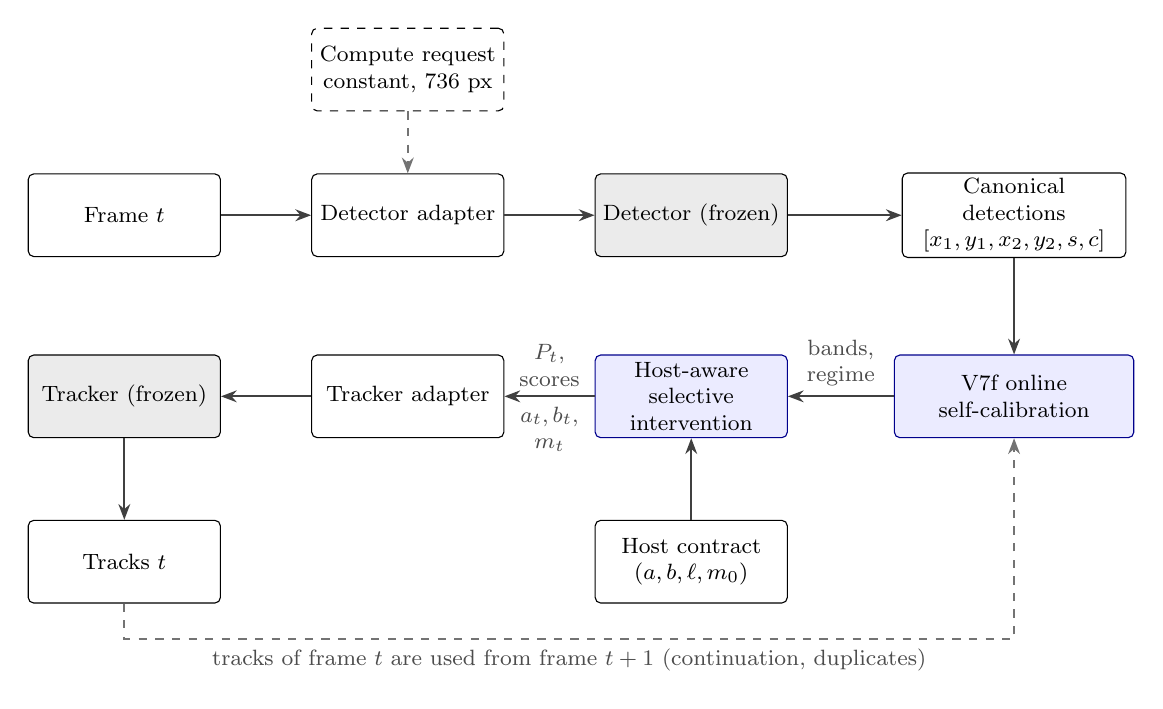
\begin{tikzpicture}[
  bx/.style={draw, rounded corners=2pt, align=center, font=\footnotesize, minimum height=1.05cm, text width=2.3cm, inner sep=2pt, fill=white},
  fz/.style={bx, fill=black!8},
  pol/.style={bx, fill=blue!8, draw=blue!55!black},
  ar/.style={-{Stealth[length=2mm]}, thick, color=black!75},
  da/.style={-{Stealth[length=2mm]}, thick, dashed, color=black!55},
  lab/.style={font=\footnotesize, color=black!70, align=center}]
\node[bx] (f) at (0,0) {Frame $t$};
\node[bx] (dad) at (3.6,0) {Detector adapter};
\node[fz] (det) at (7.2,0) {Detector (frozen)};
\node[bx, text width=2.7cm] (can) at (11.3,0) {Canonical detections\\{\footnotesize $[x_1,y_1,x_2,y_2,s,c]$}};
\node[pol, text width=2.9cm] (cal) at (11.3,-2.3) {V7f online\\self-calibration};
\node[pol] (sel) at (7.2,-2.3) {Host-aware\\selective\\intervention};
\node[bx] (tad) at (3.6,-2.3) {Tracker adapter};
\node[fz] (trk) at (0,-2.3) {Tracker (frozen)};
\node[bx] (out) at (0,-4.4) {Tracks $t$};
\node[bx] (hc) at (7.2,-4.4) {Host contract\\{\footnotesize $(a,b,\ell,m_0)$}};
\node[bx, dashed] (cmp) at (3.6,1.85) {Compute request\\{\footnotesize constant, 736 px}};
\draw[ar] (f) -- (dad); \draw[ar] (dad) -- (det); \draw[ar] (det) -- (can);
\draw[ar] (can) -- (cal);
\draw[ar] (cal) -- node[lab, above]{bands,\\regime} (sel);
\draw[ar] (sel) -- node[lab, above]{$P_t$,\\scores} node[lab, below]{$a_t,b_t,$\\$m_t$} (tad);
\draw[ar] (tad) -- (trk);
\draw[ar] (trk) -- (out);
\draw[ar] (hc) -- (sel);
\draw[da] (cmp) -- (dad);
\draw[da] (out.south) -- ++(0,-0.45) -| node[lab, pos=0.25, below]{tracks of frame $t$ are used from frame $t+1$ (continuation, duplicates)} (cal.south);
\end{tikzpicture}
\end{adjustbox}
\caption{Architecture of General AC-MOT. White boxes are translation (implementation-specific adapters) and data; blue boxes are the decision policy, which contains no detector, tracker or dataset names; grey boxes are the frozen models. The policy decides from the score stream of previous frames, the tracker's declared host contract and the tracks of the previous frame. The compute request is constant in the frozen system.}
\label{fig:arch}
\end{figure*}

\subsection{Problem formulation}\label{sec:problem}
At frame $t$ the frozen detector emits candidates $\{(\mathbf{x}_i, s_i, c_i)\}_{i=1}^{n_t}$ with boxes, scores $s_i\in(0,1)$ and class labels, down to a score floor; $z_i=\log\bigl(s_i/(1-s_i)\bigr)$ is the logit. The frozen tracker declares a host contract $(a, b, \ell, m_0)$: the score threshold of its first association, the lowest score at which it starts a track, the lowest score used by any of its association stages, and its matching tolerance (one minus its minimum overlap). A host is \emph{single-stage} when $\ell \geq \min(a,b)$ and \emph{two-stage} otherwise. For each frame the layer outputs the set $P_t$ of candidates passed to the tracker, their scores, the thresholds $(a_t, b_t)$ and the tolerance $m_t$ that the tracker uses at that frame. The requirements are: no training and no labels at deployment; one frozen configuration for every detector, tracker and dataset; causality (the thresholds of frame $t$ depend only on frames before $t$); and no change of the output when the tracker's operating point already fits the stream. The thresholds therefore cannot be fixed numbers shared by all detectors: Fig.~\ref{fig:scores} shows the same raw threshold falling at different positions in the score streams of four detectors.

\begin{figure*}[t]
\centering
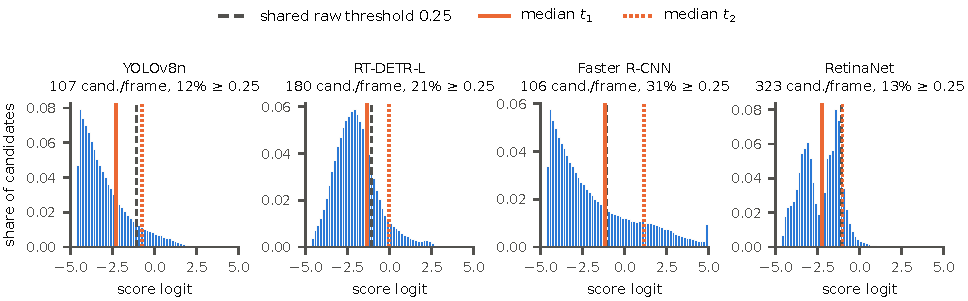
\includegraphics[width=\textwidth]{figures/fig3_score_distributions.pdf}
\caption{Score distributions of four detectors on the same frames (VisDrone2019-MOT val, 736 px, all candidates above the 0.01 floor, logits clipped to $[-5,5]$). The dashed line is the shared raw threshold 0.25; the solid and dotted lines are the medians over frames of the self-calibrated thresholds $t_1$ and $t_2$. The shared raw threshold lies between $t_1$ and $t_2$ for every detector, but at very different relative positions: just above the background split for Faster R-CNN, and just below the confident split for RetinaNet.}
\label{fig:scores}
\end{figure*}

\subsection{Canonical interfaces and adapters}\label{sec:adapters}
A detector adapter runs an implementation (Ultralytics YOLOv8n and RT-DETR-L; torchvision Faster R-CNN~\cite{ren2017fasterrcnn,lin2017fpn} and RetinaNet~\cite{lin2017focal}) with a score floor of 0.01, at most 1000 detections per frame and the detector's native suppression, keeps the person, car, bus and truck classes, and returns canonical detections $[x_1,y_1,x_2,y_2,s,c]$. A tracker adapter converts canonical detections and the layer's thresholds into the native call of a tracker (for ByteTrack, the association threshold becomes \texttt{track\_high\_thresh}, the birth threshold \texttt{new\_track\_thresh}, the tolerance \texttt{match\_thresh}; for OC-SORT, \texttt{det\_thresh} $=\min(a_t,b_t)$ and the IoU gate $1-m_t$) and returns tracks in canonical form. Adapters are translation: they may be specific to one implementation, and their only parameters are those of the native interface. The decision policy below never sees a model name. A unit test checks that the policy code contains no detector, tracker, dataset or sequence name, and the pass-through path (adapters and layer without intervention) reproduces the native hosts exactly (Sect.~\ref{sec:ablation}).

\subsection{Causal score history}\label{sec:history}
The layer keeps the logits of the candidates retained after duplicate handling in each of the last $W=\V{const.window}$ frames, one entry per frame, including empty frames. The pooled history used at frame $t$ is
\begin{equation}
H_t=\bigcup_{\tau=t-W}^{t-1}\{z_i^{\tau}: i\in K_\tau\},
\end{equation}
where $K_\tau$ is the retained set of frame $\tau$. Frame-$t$ logits enter the history only after the decision for frame $t$ has been made, so no decision uses its own frame's scores to set its thresholds, and no future frame is ever used. If $H_t$ holds fewer than \V{const.minlogits} values or has zero spread, the frame is \emph{cold} and the host's own thresholds are used.

\subsection{Nested exact Otsu thresholds}\label{sec:otsu}
For a finite set $V$ of logits sorted as $v_{(1)}\le\dots\le v_{(n)}$, the exact two-class Otsu threshold~\cite{otsu1979} is
\begin{equation}
\mathrm{Otsu}(V)=\tfrac12\bigl(v_{(k^\ast)}+v_{(k^\ast+1)}\bigr),\qquad k^\ast=\arg\max_{k}\;k\,(n-k)\,\bigl(\bar v_{1:k}-\bar v_{k+1:n}\bigr)^2,
\end{equation}
computed over all split points without histogram bins. The layer applies it twice:
\begin{equation}
t_1=\mathrm{Otsu}(H_t),\qquad t_2=\mathrm{Otsu}\bigl(\{z\in H_t: z\ge t_1\}\bigr),
\end{equation}
with $t_2=t_1$ if the second split is undefined. The first split separates background-like candidates from object-like ones; the second, computed inside the object-like part only, separates ambiguous from confident candidates, so that it does not depend on how many background candidates the detector emits. Figure~\ref{fig:otsu} shows the result on one real ten-frame window of RT-DETR-L.

\subsection{Detection bands}\label{sec:bands}
The two thresholds define three bands: \emph{primary} candidates ($z\ge t_2$) may start and continue tracks; \emph{extension} (ambiguous) candidates ($t_1\le z<t_2$) may continue existing tracks but not start new ones; \emph{reject} candidates ($z<t_1$) are not passed when the layer intervenes. Because Otsu thresholds are order statistics, the band membership of every candidate is unchanged by any increasing affine transformation of the logits, including temperature scaling. The clean regime compares the bands with the host's fixed thresholds, so V7f as a whole is not invariant to recalibration; its regime decision and its noisy-regime output are.

\begin{figure}[t]
\centering
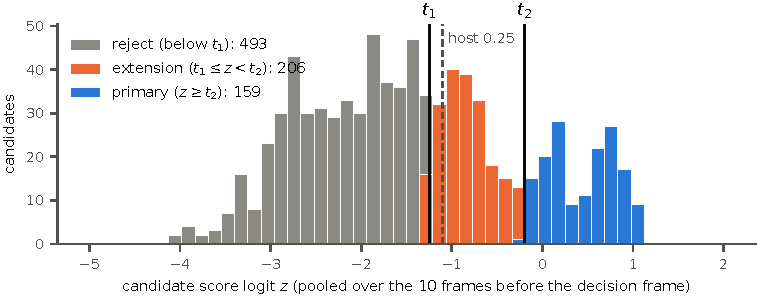
\includegraphics[width=\linewidth]{figures/fig4_nested_otsu.pdf}
\caption{Nested Otsu bands on one real window: the logits of RT-DETR-L candidates in the ten frames before one decision frame (VisDrone val sequence uav0000086, \V{fig4.pooled} candidates). The first split $t_1$ (score \V{fig4.t1score}) separates background-like from object-like candidates; the second split $t_2$ (score \V{fig4.t2score}), computed inside the object-like part only, separates extension from primary candidates. The dashed line marks the tracker's raw threshold of 0.25. Computed with the frozen thresholding function on the cached detector output; duplicate handling is not applied in this illustration.}
\label{fig:otsu}
\end{figure}

\subsection{Regime estimate: when to intervene}\label{sec:regime}
The share of confident candidates among object-like candidates,
\begin{equation}
\rho_t=\frac{\bigl|\{z\in H_t: z\ge t_2\}\bigr|}{\bigl|\{z\in H_t: z\ge t_1\}\bigr|},
\end{equation}
is high when the detector separates objects cleanly and low when its object-like scores are spread out. Before $\rho_t$ is used, an interpretability check asks whether the first split really found a background mode: if fewer candidates lie below $t_1$ than above it, the split is not interpreted as background versus objects and $\rho_t$ is set to 1. The regime uses the median over the whole stream so far,
\begin{equation}
\bar\rho_t=\operatorname{median}\{\rho_\tau:\tau\le t,\ \tau\ \text{not cold}\},\qquad \text{clean if } \bar\rho_t\ge \tfrac12,\ \text{noisy otherwise},
\end{equation}
where each $\rho_\tau$ is computed from frames before $\tau$. The cumulative median makes the regime a property of the stream rather than of a few frames.

\subsection{Clean regime: minimal intervention}\label{sec:clean}
On a clean stream the layer keeps the tracker's operating point and only lowers a threshold that lies above the stream's confident band:
\begin{equation}
a_t=\min\bigl(a,\sigma(t_2)\bigr),\qquad b_t=\min\bigl(b,\sigma(t_2)\bigr),
\end{equation}
with $\sigma$ the logistic function. No candidate is discarded by the bands (only cross-class duplicates are removed, Sect.~\ref{sec:dup}), raw scores are passed unchanged, and the host's own low-score stage keeps working. By construction the clean regime never raises a host threshold; a unit test asserts this property.

\subsection{Noisy regime: intervention}\label{sec:noisy}
On a noisy stream the layer replaces the host's operating point by the stream's bands: candidates below $t_1$ are discarded, the association and birth thresholds both move to $t_2$, and the scores of the passed candidates are remapped by rank so that the host's thresholds become meaningful,
\begin{equation}
s'_i=\begin{cases}0.5+0.5\,u_i & z_i\ge t_2,\\ 0.1+0.4\,u_i & t_1\le z_i<t_2,\end{cases}\qquad a_t=b_t=0.5,
\end{equation}
where $u_i\in(0,1)$ is the mid-rank of $s_i$ in a reference sample of retained raw scores (frame~1 and every \V{const.ecdfstride}th frame, last \V{const.ecdfwin} samples). Primary candidates thus reach the host above its association and birth thresholds; extension candidates reach a two-stage host's low-score stage but cannot start tracks. The remapping is applied only in noisy frames; in clean and cold frames the raw scores are passed.

\subsection{Crowd-safe duplicate handling}\label{sec:dup}
Overlapping candidates are a frequent symptom of a noisy detector, but in crowded scenes overlapping boxes are often distinct objects. In noisy frames, candidates are visited in descending score, and a candidate overlapping an already kept one (IoU $>0.5$) is dropped \emph{unless} it is claimed (IoU $\ge 0.5$) by a different track of frame $t-1$ than the kept candidate. In clean and cold frames only cross-class duplicates are removed (overlap above 0.5 with a kept candidate of another class), so single-class streams pass unchanged.

\subsection{Track continuation for lower-scored detections}\label{sec:rescue}
A single-stage tracker ignores every candidate below its threshold, even one that continues an existing track. When a track of frame $t-1$ is not covered by any candidate the host will use (IoU $\ge 0.5$), the highest-scored candidate that overlaps it (IoU $\ge 0.5$), lies in the object-like part of the stream (raw score $\ge\sigma(t_1)$) and would otherwise be invisible to the host receives a score just above the lowest score the host uses at that frame (margin \V{const.margin}). For a single-stage host that floor is $\min(a_t,b_t)$; for a two-stage host it is $\ell$, so the host's own low-stage bound is respected. For a two-stage host the lifted score stays below the birth threshold, so the continuation cannot start a track; for a single-stage host it reaches the host's only threshold, so an unmatched continuation candidate could start one. When the interpretability check found no background mode, every candidate of a single-stage host counts as object-like.

\subsection{Motion-conditioned matching tolerance}\label{sec:motion}
When frames are available, a global motion cue $c_t$ (phase-correlation shift of quarter-resolution grey frames, normalized by the image diagonal~\cite{reddy1996phasecorr}) is compared with the median of its previous values, $r_t=c_t/\operatorname{median}(c_{t-100},\dots,c_{t-1})$ after \V{const.warmup} warm-up values. In noisy frames only, the matching tolerance becomes $m_t=\min\bigl(0.95,\,1-(1-m_0)/\max(1,r_t)\bigr)$. The rule is inactive when no frames are available, which is the case for every MOT17 and external-tracker experiment of this paper.

\subsection{Host contract and host-aware selective intervention}\label{sec:host}
Table~\ref{tab:contracts} lists the contracts declared by the tested trackers. The contract contains numbers only; no field names the tracker. Everything that distinguishes trackers enters through it: whether a low-score stage exists (single- versus two-stage), whether tracks start at a different threshold than they associate, and the matching tolerance. The policy therefore needs no branch of the form ``if the tracker is ByteTrack''. Host awareness acts in three places: the clean regime keeps the declared operating point; the continuation floor follows the declared lowest stage; and the noisy regime maps its decisions onto the declared thresholds. We call the resulting behaviour \emph{host-aware selective intervention}. It is a design property, not a guarantee: Sect.~\ref{sec:boundary} reports cases in which the regime decision was wrong and the layer degraded a tracker.

\begin{table*}[!htbp]
\centering
\caption{Host contracts: the operating point each tracker declares to the layer (association threshold, birth threshold, lowest score used by any association stage, matching tolerance). $\tau$ is the tracker's own published threshold. A host is single-stage when its lowest stage equals its association/birth threshold. The contract carries no tracker identity.}
\label{tab:contracts}
\footnotesize
\setlength\tabcolsep{3.5pt}
\begin{tabular}{p{5.0cm}lcccl}
\toprule
Tracker (setting) & Type & assoc & birth & low & match \\
\midrule
ByteTrack (library default; also BoT-SORT) & two-stage & 0.25 & 0.25 & 0.1 & 0.8 \\
ByteTrack (official MOT17) & two-stage & 0.6 & 0.7 & 0.1 & 0.8 \\
SparseTrack & two-stage & $\tau$ & $\tau+0.1$ & 0.1 & published \\
BoostTrack & two-stage & $\tau$ & $\tau$ & 0.1 & $1-$IoU gate \\
Hybrid-SORT & two-stage & $\tau$ & $\tau$ & 0.1 & $1-$IoU gate \\
OC-SORT & single-stage & 0.6 & 0.6 & 0.6 & 0.7 \\
PD-SORT & single-stage & $\tau$ & $\tau$ & $\tau$ & $1-$IoU gate \\
C-TWiX (MOT17 / KITTI / DanceTrack) & single-stage & 0.5 & 0.7 / 0.5 / 0.9 & 0.5 & not mapped \\
TrackTrack & two-view & $\tau_{\mathrm{det}}$ & $\tau_{\mathrm{init}}$ & 0.1 & not mapped \\
\botrule
\end{tabular}
\end{table*}


\subsection{Causality}\label{sec:causality}
Every threshold, band and regime decision for frame $t$ uses statistics of frames before $t$. Duplicate handling and continuation use the geometry of frame $t$ and the host's tracks of frame $t-1$; the matching tolerance uses the image cue of frame $t$ normalized by the history of earlier frames. Frame-$t$ data update the state only after the decision. Unit tests run on the frozen V7f configuration assert that the operating point and the regime of frame $t$ do not change when the candidates of frame $t$ are replaced, that future frames do not change past decisions, that a reset equals a fresh layer, that clean and cold frames never raise host thresholds or change the matching tolerance, and that the regime decisions are invariant to increasing affine recalibration of the logits.

\subsection{Algorithm and complexity}\label{sec:algorithm}
Algorithm~\ref{alg:v7f} gives the complete per-frame procedure. With $n$ candidates per frame, $k$ previous tracks and window $W$, exact Otsu on the pooled history costs $O(Wn\log Wn)$, duplicate handling $O(n^2)$, the track claims and continuation $O(nk)$, and the rank remap $O(n\log M)$ for a reference sample of size $M$. The frozen implementation recomputes the cumulative median of $\rho$ over all previous frames, which adds $O(T)$ at frame $T$; a two-heap median would reduce this to $O(\log T)$ without changing any decision. The motion cue adds one phase correlation on a quarter-resolution frame. Measured costs are in Sect.~\ref{sec:runtime}.

\begin{algorithm}[t]
\caption{V7f decision for frame $t$ (frozen policy)}\label{alg:v7f}
\footnotesize
\begin{algorithmic}[1]
\Require candidates $\{(\mathbf{x}_i,s_i,c_i)\}$ of frame $t$; host contract $(a,b,\ell,m_0)$; tracks $\mathcal{T}_{t-1}$; motion cue $c_t$ (optional); state (window of retained logits, $\rho$ history, rank reference, motion history)
\State $z_i\gets\log(s_i/(1-s_i))$; \ $H\gets$ pooled logits of frames $t-W,\dots,t-1$
\If{$|H|<3$ or $H$ has zero spread} \Comment{cold}
  \State $(a_t,b_t)\gets(a,b)$; no discard; regime $\gets$ cold
\Else
  \State $t_1\gets\mathrm{Otsu}(H)$; \ $t_2\gets\mathrm{Otsu}(\{z\in H:z\ge t_1\})$
  \State $\rho\gets|\{z\ge t_2\}|/|\{z\ge t_1\}|$; \ \textbf{if} $|\{z<t_1\}|<|\{z\ge t_1\}|$ \textbf{then} $\rho\gets 1$
  \State append $\rho$ to history; \ $\bar\rho\gets$ median of history
  \If{$\bar\rho\ge\frac12$} \Comment{clean: keep host operating point}
     \State $a_t\gets\min(a,\sigma(t_2))$; \ $b_t\gets\min(b,\sigma(t_2))$; no discard
  \Else \Comment{noisy: intervene}
     \State discard threshold $\gets t_1$; \ $a_t, b_t\gets t_2$ (on the logit scale)
  \EndIf
\EndIf
\State $K\gets$ duplicate handling (noisy: crowd-safe rule with $\mathcal{T}_{t-1}$; otherwise cross-class rule only)
\State $P\gets\{i\in K: z_i\ge$ discard threshold$\}$
\If{noisy} rank-remap scores of $P$ ($0.5+0.5u$ primary, $0.1+0.4u$ extension); \ $(a_t,b_t)\gets(0.5,0.5)$
\Else \ pass raw scores; \ $(a_t,b_t)\gets(\sigma(a_t),\sigma(b_t))$ \EndIf
\State floor $\gets\min(a_t,b_t)$ if $\ell\ge\min(a,b)$ else $\ell$
\For{each track $j\in\mathcal{T}_{t-1}$ not covered (IoU $\ge 0.5$) by a candidate above the floor}
  \State lift the best-scored overlapping candidate with raw score $\ge\sigma(t_1)$ to floor $+\,10^{-3}$ (not in cold frames)
\EndFor
\State $m_t\gets m_0$; \ \textbf{if} noisy and $c_t$ given: $m_t\gets\min(0.95,1-(1-m_0)/\max(1,r_t))$
\State \textbf{after the decision:} push logits of $K$ to the window; update rank reference and motion history
\State \Return $P$, scores, $(a_t,b_t)$, $m_t$ to the tracker adapter
\end{algorithmic}
\end{algorithm}

\subsection{Constants}\label{sec:constants}
Table~\ref{tab:constants} lists every constant of the frozen policy. The window, the overlap rule, the rank ranges and the safety bounds are structural or conventional; the thresholds $t_1$ and $t_2$ are computed online; the host values are declared by the tracker. The regime boundary $\bar\rho_t\ge\frac12$ and the switches between the mechanisms were fixed during development on labelled development data. ``Training-free'' in this paper therefore means that nothing is fitted and no label is needed at deployment, not that the design never saw labels.

\begin{tableorg}[!htbp]
\centering
\caption{Constants of the frozen V7f layer (\texttt{acmot\_v7.py} and \texttt{configs/universal\_acmot\_policy\_v7.json} at tag \texttt{universal-acmot-v7-freeze}). No constant names a detector, tracker, dataset or sequence; none is fitted at deployment. The design constants were fixed during development, which used labelled development data.}
\label{tab:constants}
\footnotesize
\setlength\tabcolsep{3.5pt}
\begin{adjustbox}{max width=\linewidth}
\begin{tabular}{p{3.7cm}p{2.0cm}p{4.0cm}p{2.6cm}}
\toprule
Quantity & Value & Nature & Location \\
\midrule
History window $W$ (frames) & 10 & structural; insensitivity checked in development (5/20) & config \texttt{window} \\
Minimum pooled logits for valid bands & 3 & structural (Otsu needs a split) & \texttt{\_bands} \\
Thresholds $t_1$, $t_2$ & data & online, nested exact Otsu & \texttt{nested\_otsu} \\
Regime boundary & $\bar\rho_t \geq 0.5$ & design constant chosen on development data & \texttt{step} \\
Overlap rule (duplicates, track claim, rescue) & IoU 0.5 & conventional correspondence threshold & config \texttt{dup\_iou} \\
Rank remap (noisy regime) & $0.5+0.5u$ / $0.1+0.4u$ & structural (order-preserving, two ranges) & \texttt{step} \\
ECDF reference: stride / samples & 10 / 20 & structural & \texttt{step} \\
Motion history / warm-up & 100 / 5 & structural & config \texttt{hist}, \texttt{warmup} \\
Matching-tolerance cap & 0.95 & safety bound & \texttt{step} \\
Rescue margin above the host's lowest usable score & $10^{-3}$ & numerical margin & \texttt{step} \\
Clipping (ECDF / logit) & $10^{-6}$ / $10^{-9}$ & numerical & \texttt{\_ecdf}, \texttt{logit} \\
Host thresholds and matching tolerance & declared & host contract (Table~\ref{tab:contracts}) & host adapter \\
\botrule
\end{tabular}
\end{adjustbox}
\end{tableorg}


%==========================================================================================
\section{Experimental Protocol}\label{sec:protocol}
%==========================================================================================
\paragraph{Data and roles.} Table~\ref{tab:protocol} lists the settings. VisDrone2019-MOT~\cite{zhu2022visdrone} test-dev (\V{s1.nseq} sequences, \V{s1.frames} frames) and UAVDT~\cite{du2018uavdt} test (\V{uav.nseq} sequences, \V{uav.frames} frames) evaluate Stage 1. VisDrone2019-MOT val (\V{vd.nseq} sequences, \V{vd.frames} frames), KITTI tracking training~\cite{geiger2012kitti} and MOT17~\cite{milan2016mot16} val-half are development data of V7f. External systems were run on MOT17 val-half, KITTIMOTS val and DanceTrack val~\cite{sun2022dancetrack}. The status of every result is marked: \emph{development} (the data or the host were visible while V7f was designed), \emph{predeclared external} (selected and declared in the freeze commit of V7f, evaluated once), \emph{post-freeze external} (selected after the freeze under a written protocol, evaluated once), and \emph{unseen detector} (a detector family never used in the project before the freeze of General AC-MOT, evaluated under a transfer lock committed before any of its tracking metrics existed). Only DanceTrack is a dataset that no development run used. Detections come from five detectors, YOLOv8n, RT-DETR-L and RetinaNet run by us, the published YOLOX-X models of the MOT17 and DanceTrack trackers, and PermaTrack, and from the released DanceTrack detection set of TrackTrack; Faster R-CNN appears only in the raw-threshold analysis of Sect.~\ref{sec:res_transfer}.

\begin{table*}[!htbp]
\centering
\caption{Evaluation settings and the role of each. `Development' data were visible while the corresponding system was designed; `external' systems were run once with the frozen policy. No result in this paper is a test-server or leaderboard submission.}
\label{tab:protocol}
\footnotesize
\setlength\tabcolsep{3.5pt}
\begin{tabular}{p{2.9cm}p{1.8cm}p{2.0cm}p{2.4cm}p{2.6cm}p{2.3cm}}
\toprule
Data & System & Detector(s) & Tracker(s) & Role & Evaluation \\
\midrule
VisDrone2019-MOT test-dev & Stage 1 & YOLOv8n & ByteTrack & held-out, locked one-shot (Stage 1) & custom class-agnostic \\
UAVDT test & Stage 1 & YOLOv8n & ByteTrack & frozen transfer, no retuning (Stage 1) & UAVDT adapter, IoU 0.5 \\
VisDrone2019-MOT val (7 seq.) & V7f, General AC-MOT & YOLOv8n, RT-DETR-L & ByteTrack, BoT-SORT, OC-SORT & development & internal and official-compatible \\
VisDrone2019-MOT val (7 seq.) & General AC-MOT & RetinaNet & ByteTrack, BoT-SORT & unseen detector (locked), development sequences & internal and official-compatible \\
KITTI tracking training (21 seq.) & V7f & YOLOv8n, RT-DETR-L & ByteTrack, BoT-SORT, OC-SORT & development & KITTI HOTA (car/pedestrian mean) \\
MOT17 val-half (7 seq.) & V7f & YOLOX-X (published) & SparseTrack, BoostTrack, ByteTrack, OC-SORT & development & TrackEval, internal \\
MOT17 val-half (7 seq.) & V7f & YOLOX-X (published) & PD-SORT, Hybrid-SORT & predeclared external & TrackEval, internal \\
MOT17 val-half / KITTIMOTS val / DanceTrack val & V7f & released detections (incl. PermaTrack) & C-TWiX, TrackTrack & post-freeze external & TrackEval, internal \\
\botrule
\end{tabular}
\end{table*}


\paragraph{Freezes and locks.} Stage 1 was frozen at tag \texttt{v1.0.0-acmot-frozen} before its locked test-dev run, in which each system ran once in its own T4 session. V7f was frozen at tag \texttt{universal-acmot-v7-freeze} with a file-hash lock (\texttt{research/V7\_POLICY\_LOCK.json}); General AC-MOT at tag \texttt{general-acmot-g1-freeze} with a lock over the policy, adapters, host contracts and runners (\texttt{research/GENERAL\_ACMOT\_G1\_LOCK.json}). Every file in both locks matches its recorded hash in the evidence snapshot used for this paper. Nothing was retuned on any transfer target.

\paragraph{Metrics and evaluation.} We report HOTA~\cite{luiten2021hota}, MOTA~\cite{bernardin2008clear} and IDF1~\cite{ristani2016idf1} (in percentage points), identity switches (IDS), false positives and negatives, precision and recall, computed with TrackEval at commit \texttt{\V{s1.trackeval}}. Stage-1 VisDrone and UAVDT results use a custom class-agnostic protocol (VisDrone ground-truth categories 1, 4, 5, 6 and 9, score 1, occlusion and truncation below 2) that is not the official VisDrone toolkit. For General AC-MOT on VisDrone we additionally report an \emph{official-compatible} evaluation, a port of the VisDrone MOT toolkit (class-aware, ignored regions removed) with HOTA added; it is not the evaluation server. COCO detectors have no ``van'' class, so van objects count as misses under that protocol. MOT17, KITTI and DanceTrack results are validation-split evaluations in our environment; none is a test-server submission. A sequence with MOTA $<0$ is called \emph{catastrophic}.

\paragraph{Statistics.} Differences are paired over sequences (or detector--sequence cells for pooled results) and reported with percentile 95\% bootstrap intervals: 5,000 resamples with seed 42 for Stage 1 and 10,000 resamples with seed 42 for all later results. Each interval is descriptive and per comparison, without correction for multiple comparisons. W/T/L counts the sequences won, tied and lost.

\paragraph{Hardware.} Stage-1 timing was measured on an NVIDIA Tesla T4 as processing throughput on decoded frames. V7f and General AC-MOT were timed on CPUs only (Sect.~\ref{sec:runtime}); no GPU timing of them is reported.

%==========================================================================================
\section{Results}\label{sec:results}
%==========================================================================================
\subsection{Stage 1: AC-MOT worked}\label{sec:res_stage1}
Table~\ref{tab:stage1} gives the locked test-dev comparison. The calibrated controller raised HOTA by \Vz{s1.qb.dHOTA}, MOTA by \Vz{s1.qb.dMOTA} and IDF1 by \Vz{s1.qb.dIDF1} over the static default and won on all \V{s1.nseq} sequences (W/T/L \V{s1.qb.wtl}); per-sequence gains ranged from \V{s1.qb.seqmin} to \V{s1.qb.seqmax} HOTA points. The gain came mostly from recall: false negatives fell by \V{s1.qb.dFN}, false positives rose by \V{s1.qb.dFP}, and the identity-switch reduction (\V{s1.qb.dIDS_reduction}) was not significant. Against the hand-designed SCI controller it gained \Vz{s1.qh.dHOTA} HOTA but had more identity switches (\V{s1.q.IDS} against \V{s1.heur.IDS}; reduction \Vz{s1.qh.dIDS_reduction}), so it did not dominate the earlier controller on every metric. Frozen and unchanged, it transferred to UAVDT with \Vz{uav.qb.dHOTA} HOTA (W/T/L \V{uav.qb.wtl}). The controller ran at \V{s1.q.FPS} frames per second of processing on a T4; this figure excludes JPEG decoding (\V{t4.decode}~ms per frame), with which serialized playback of a matched static configuration reached \V{t4.playfps} frames per second, and repeated measurements of one configuration in different sessions differed by several frames per second.

\begin{tableorg}[!htbp]
\centering
\caption{Stage 1: the scene-adaptive AC-MOT controller with YOLOv8n and ByteTrack. Custom class-agnostic protocol (TrackEval), not the official VisDrone toolkit. Intervals: paired sequence bootstrap, 5,000 resamples, seed 42. FPS is processing throughput on decoded frames on a Tesla T4, each system in its own session.}
\label{tab:stage1}
\footnotesize
\setlength\tabcolsep{3.5pt}
\begin{adjustbox}{max width=\linewidth}
\begin{tabular}{p{4.4cm}rrrrrrr}
\toprule
System & HOTA & MOTA & IDF1 & IDS & FP & FN & FPS \\
\midrule
\multicolumn{8}{l}{\textit{VisDrone2019-MOT test-dev, 17 sequences, locked one-shot comparison}} \\
Static operating point, default tracker & 28.43 & 19.73 & 32.72 & 1,235 & 16,308 & 155,051 & 36.53 \\
Hand-designed SCI controller & 32.70 & 23.24 & 39.52 & 1,061 & 25,025 & 138,967 & 41.96 \\
Calibrated SCI controller (AC-MOT) & 33.84 & 26.95 & 41.55 & 1,184 & 19,029 & 136,858 & 38.98 \\
$\Delta$ AC-MOT $-$ static & +5.41 & +7.22 & +8.82 & \ensuremath{-}51 & +2,721 & \ensuremath{-}18,193 & -- \\
\quad 95\% CI & [+4.13, +6.90] & [+5.44, +9.29] & [+6.90, +11.05] & & & & \\
$\Delta$ AC-MOT $-$ hand-designed & +1.14 & +3.71 & +2.03 & +123 & \ensuremath{-}5,996 & \ensuremath{-}2,109 & -- \\
\quad 95\% CI & [+0.14, +2.27] & [+2.39, +5.19] & [+0.59, +3.77] & & & & \\
\midrule
\multicolumn{8}{l}{\textit{UAVDT test, 20 sequences, frozen controller, no retuning}} \\
Static operating point, default tracker & 24.08 & 13.84 & 27.89 & 558 & 22,974 & 270,189 & 65.01 \\
Calibrated SCI controller (AC-MOT) & 28.39 & 17.40 & 34.45 & 321 & 22,896 & 258,376 & 58.35 \\
$\Delta$ AC-MOT $-$ static & +4.305 & +3.558 & +6.565 & \ensuremath{-}237 & \ensuremath{-}78 & \ensuremath{-}11,813 & -- \\
\quad 95\% CI & [+2.740, +5.709] & [+1.452, +5.807] & [+3.808, +8.822] & & & & \\
\botrule
\end{tabular}
\end{adjustbox}
\par\smallskip\parbox{\linewidth}{\footnotesize Identity-switch reduction with 95\% CI: AC-MOT vs static +51 [\ensuremath{-}114, +219] (test-dev) and +237 [+104, +377] (UAVDT); AC-MOT vs hand-designed \ensuremath{-}123 [\ensuremath{-}244, \ensuremath{-}14] (negative: more switches). Sequences won/tied/lost on HOTA: 17/0/0 and 13/0/4 on test-dev, 15/2/3 on UAVDT. FP/FN/IDS differences are count differences without intervals.}
\end{tableorg}


\subsection{Why AC-MOT worked: operating-point calibration}\label{sec:res_attribution}
The calibrated controller hardly switched: on validation it ran at a mean input of \V{val.q.res} px, a mean confidence of \V{val.q.conf} and a constant NMS IoU of \V{val.q.nms}. We therefore ran, post hoc, the matched static operating point (\V{ms.a0.res} px, confidence \V{ms.a0.conf}, NMS \V{ms.a0.nms}, tuned tracker) on test-dev (Table~\ref{tab:attribution}). It reached \V{ms.a0.HOTA} HOTA against \V{s1.q.HOTA} for the controller (\Vz{ms.dHOTA}); MOTA, IDF1 and IDS differences also had intervals containing zero. On validation, the step from the static default to the tuned tracker profile added \V{val.d_tracker} HOTA, the calibrated static operating point a further \V{val.d_operating}, and scene switching \V{val.d_switch}. This matched-static test is post hoc and is used only for attribution, not as a fourth system of the locked comparison.

\begin{table*}[!htbp]
\centering
\caption{Attribution of the Stage-1 gain. The matched static operating point reproduces the calibrated controller within the resolution of the test; on validation, almost all of the gain over the static default comes from the tracker profile and the calibrated operating point, not from frame-to-frame switching.}
\label{tab:attribution}
\footnotesize
\setlength\tabcolsep{3.5pt}
\begin{tabular}{p{6.2cm}rrrr}
\toprule
System & HOTA & MOTA & IDF1 & IDS \\
\midrule
\multicolumn{5}{l}{\textit{Held-out test-dev (post hoc attribution, 17 sequences)}} \\
Calibrated SCI controller (AC-MOT) & 33.84 & 26.95 & 41.55 & 1,184 \\
Matched static point (960 px, conf 0.35, NMS 0.35) & 33.93 & 27.00 & 41.77 & 1,197 \\
$\Delta$ controller $-$ matched static [95\% CI] & \textminus{}0.09 [\textminus{}0.25, +0.06] & \textminus{}0.05 [\textminus{}0.25, +0.16] & \textminus{}0.23 [\textminus{}0.50, +0.02] & +13 [\textminus{}23, +46]$^{a}$ \\
\midrule
\multicolumn{5}{l}{\textit{Validation (VisDrone2019-MOT val, 7 sequences): decomposition of the gain, HOTA}} \\
Static 640 px, conf 0.25, default tracker & 29.84 & \multicolumn{3}{l}{reference} \\
+ tuned tracker profile & 30.86 & \multicolumn{3}{l}{+1.03} \\
+ calibrated static operating point (960 px, 0.35, 0.35) & 36.08 & \multicolumn{3}{l}{+5.21} \\
+ scene switching (calibrated controller) & 36.11 & \multicolumn{3}{l}{+0.03} \\
\botrule
\end{tabular}
\par\smallskip\parbox{\linewidth}{\scriptsize $^{a}$ IDS reduction (positive = fewer switches for the controller). The calibrated controller ran at a mean input of 957 px, mean confidence 0.34 and constant NMS 0.35 on validation; the matched static point was run on 2026-09-18, after the freeze, and is used only for attribution.}
\end{table*}


The reading is not that the SCI was useless. The SCI and its validation-only calibration were the procedure that found an operating point (high resolution, a higher confidence threshold, strong suppression) far better than the default; the hand-designed SCI controller had itself raised HOTA over the static default (\V{s1.heur.HOTA} against \V{s1.base.HOTA}; no interval was recorded for this pair). What the attribution shows is that, once found, a calibrated operating point carried the gain, and that operating-point calibration is the most transferable mechanism inside AC-MOT.

\subsection{Why the calibration does not transfer directly}\label{sec:res_transfer}
\paragraph{Scene indices are pipeline-specific.} When the AC-MOT design was placed on a second pipeline (the U2MOT tracker~\cite{liu2023u2mot} with its authors' YOLOX-X detector on VisDrone), the SCI computed on that pipeline's validation data ranged from \V{u2.sci_lo} to \V{u2.sci_hi}, whereas the frozen switching thresholds were \V{u2.bound_lo} and \V{u2.bound_hi}: every frame would have fallen into the hardest tier. A separately recalibrated controller of the same design, frozen before its test-dev run, changed HOTA by \Vz{u2.dHOTA} against the authors' static operating point (W/T/L \V{u2.wtl}; post hoc TrackEval rescore of outputs evaluated with the U2MOT repository protocol, 10,000 resamples, seed 0).

\paragraph{Raw scores are detector-specific.} Table~\ref{tab:rawscale} and Fig.~\ref{fig:scores} show four COCO detectors on the same VisDrone frames at the same input size and with the same tracker thresholds. Their score streams differ in density (from \V{fig3.fasterrcnn.perframe} to \V{fig3.retinanet.perframe} candidates per frame) and in where object-like candidates sit: the median self-calibrated thresholds $\sigma(t_2)$ range from \V{fig3.retinanet.t2} (RetinaNet) to \V{fig3.fasterrcnn.t2} (Faster R-CNN). With the shared raw threshold of 0.25, YOLOv8n had no catastrophic sequence, while RT-DETR-L had \V{raw.rtdetr.cat}, RetinaNet \V{raw.retinanet.cat} and Faster R-CNN \V{raw.fasterrcnn.cat}; precision ranged from \V{raw.retinanet.Precision} to \V{raw.yolov8.Precision}.

\begin{tableorg}[!htbp]
\centering
\caption{One raw threshold, four detectors: VisDrone2019-MOT val (7 sequences, 2,846 frames), 736 px input, score floor 0.01, ByteTrack with its library default thresholds (0.25). Columns 2--5 describe the cached detector streams: candidates per frame, share of candidates with score $\geq 0.25$, and the median over frames of the self-calibrated thresholds $t_1$ and $t_2$ (nested Otsu on the logits of the ten previous frames, shown as scores). Columns 6--10: tracking with the raw threshold (internal protocol); `Cat.' counts sequences with MOTA $<0$.}
\label{tab:rawscale}
\footnotesize
\setlength\tabcolsep{3.5pt}
\begin{adjustbox}{max width=\linewidth}
\begin{tabular}{lrrrrrrrrr}
\toprule
Detector & Cand./frame & $\geq0.25$ (\%) & $\sigma(t_1)$ & $\sigma(t_2)$ & HOTA & MOTA & Prec. & Rec. & Cat. \\
\midrule
YOLOv8n & 107 & 11.8 & 0.09 & 0.32 & 31.72 & 17.04 & 68.90 & 32.04 & 0 \\
RT-DETR-L & 180 & 20.7 & 0.21 & 0.49 & 36.76 & \ensuremath{-}6.24 & 47.95 & 58.33 & 5 \\
Faster R-CNN R50-FPN v2 & 106 & 30.6 & 0.24 & 0.76 & 34.97 & \ensuremath{-}9.56 & 46.50 & 54.22 & 6 \\
RetinaNet R50-FPN v2 & 323 & 12.9 & 0.10 & 0.27 & 27.9 & \ensuremath{-}12.6 & 43.1 & 36.3 & 3 \\
\botrule
\end{tabular}
\end{adjustbox}
\par\smallskip\parbox{\linewidth}{\footnotesize Stream statistics are computed from the published detector caches (release assets \texttt{v7-dev-assets-1} and \texttt{sci-v7f-unseen-1}, checked by SHA-256) with the frozen thresholding function; duplicate handling is not applied in these statistics. RetinaNet entered the project only after the V7f freeze.}
\end{tableorg}



\paragraph{Fixed thresholds break when the score scale moves.} On MOT17 with published YOLOX-X detections, multiplying every score by 0.5 drove ByteTrack (official setting) to \V{cal.byoff.scale05.native} and OC-SORT to \V{cal.oc.scale05.native} HOTA, because no detection reached their fixed thresholds (Table~\ref{tab:calib}); a cubic reshaping $s^3$ reduced them to \V{cal.byoff.pow3.native} and \V{cal.oc.pow3.native} HOTA, against \V{mot.byoff.base.HOTA} and \V{mot.oc.base.HOTA} on the unchanged stream. A per-detector threshold would repair each case but is exactly the per-system tuning that the layer must avoid.

\paragraph{From these findings to the design.}\label{sec:barrier} The layer therefore needs thresholds that come from the score stream itself, statistics that do not depend on the score scale, and causal updates. Earlier designs in this project tested these requirements one at a time: a histogram normalizer with a ratio gate, an order-only score transform with a global gate, and a version with global constants selected on VisDrone. The last training-free predecessor, which always applied self-calibrated nested-Otsu bands, repaired noisy streams but, added to two strong published trackers, cost SparseTrack \Vz{v6.sparse.dHOTA} and BoostTrack \Vz{v6.boost.dHOTA} HOTA on MOT17. The missing element was a decision about \emph{when not to intervene}, which became the regime estimate and the host contract of V7f.

\subsection{General AC-MOT on development detectors}\label{sec:res_dev}
Table~\ref{tab:central} collects every native-versus-V7f result; Fig.~\ref{fig:forest} plots the HOTA differences with their intervals, and Fig.~\ref{fig:matrix} arranges them as a detector--tracker matrix.

\begin{sidewaystable}[!htbp]
\centering
\caption{Central result: the host alone versus the host with the frozen layer, for every detector--tracker--dataset combination with a recorded result. HOTA, MOTA, IDF1 in points; $\Delta$ = host + V7f $-$ host alone.}
\label{tab:central}
\scriptsize
\setlength\tabcolsep{3.5pt}
\begin{tabular}{lllrrlrrrlll}
\toprule
Detector & Tracker & St. & Host & +V7f & $\Delta$HOTA [95\% CI] & $\Delta$MOTA & $\Delta$IDF1 & $\Delta$IDS & FP & FN & Prec. / Rec. \\
\midrule
\multicolumn{12}{l}{\textit{VisDrone val-7}} \\
YOLOv8n & ByteTrack & D & 31.72 & 33.89 & +2.17 [+1.20, +3.58] & +1.07 & +3.90 & \textminus{}115 & 9,740$\to$9,552 & 45,768$\to$45,351 & 68.90$\to$69.72 / 32.04$\to$32.66 \\
RT-DETR-L & ByteTrack & D & 36.76 & 41.06 & +4.30 [+2.25, +6.42] & +27.27 & +6.13 & \textminus{}671 & 42,646$\to$14,074 & 28,065$\to$38,946 & 47.95$\to$66.86 / 58.33$\to$42.17 \\
YOLOv8n & BoT-SORT & D & 35.99 & 36.60 & +0.61 [\textminus{}0.05, +1.54] & +0.94 & +0.83 & \textminus{}54 & 11,637$\to$10,721 & 43,792$\to$44,127 & 66.9$\to$68.4 / 35.0$\to$34.5 \\
RT-DETR-L & BoT-SORT & D & 41.41 & 43.56 & +2.15 [+0.16, +4.50] & +34.88 & +2.35 & \textminus{}274 & 51,836$\to$16,242 & 24,310$\to$36,691 & 45.4$\to$65.4 / 63.9$\to$45.5 \\
YOLOv8n & OC-SORT & D & 19.04 & 33.90 & +14.86 [+12.32, +19.50] & +10.23 & +20.18 & +75 & 798$\to$6,724 & 60,423$\to$47,531 & 89.7$\to$74.7 / 10.3$\to$29.4 \\
RT-DETR-L & OC-SORT & D & 35.24 & 42.00 & +6.76 [+2.88, +11.82] & +2.45 & +9.75 & \textminus{}52 & 2,736$\to$8,185 & 48,710$\to$41,660 & 87.2$\to$75.8 / 27.7$\to$38.1 \\
RetinaNet & ByteTrack & U & 27.92 & 31.93 & +4.01 [+2.25, +5.46] & +9.12 & +5.81 & \textminus{}158 & 32,229$\to$26,911 & 42,892$\to$42,226 & 43.1$\to$48.3 / 36.3$\to$37.3 \\
RetinaNet & BoT-SORT & U & 31.73 & 34.67 & +2.94 [+1.28, +4.54] & +11.00 & +4.55 & \textminus{}86 & 37,619$\to$30,274 & 40,306$\to$40,327 & 41.8$\to$47.2 / 40.1$\to$40.1 \\
\multicolumn{12}{l}{\textit{KITTI train}} \\
YOLOv8n & ByteTrack & D & 45.31 & 45.37 & +0.06 [\textminus{}1.19, +1.24] & \textminus{}1.87 & +1.49 & \textminus{}271 & n/r & n/r & n/r / n/r \\
YOLOv8n & BoT-SORT & D & 49.21 & n/r & \textminus{}1.02 [\textminus{}2.43, +0.25] & \textminus{}2.43 & +0.35 & \textminus{}227 & n/r & n/r & n/r / n/r \\
YOLOv8n & OC-SORT & D & 36.27 & 44.17 & +7.91 [+5.47, +9.98] & +9.40 & +9.60 & +79 & n/r & n/r & n/r / n/r \\
RT-DETR-L & ByteTrack & D & 50.73 & 51.64 & +0.91 [+0.22, +1.55] & +5.98 & +3.87 & \textminus{}297 & n/r & n/r & n/r / n/r \\
RT-DETR-L & BoT-SORT & D & 53.91 & n/r & +0.61 [\textminus{}0.39, +1.61] & +7.86 & +3.10 & \textminus{}226 & n/r & n/r & n/r / n/r \\
RT-DETR-L & OC-SORT & D & 52.64 & 52.83 & +0.19 [\textminus{}0.57, +1.19] & \textminus{}0.57 & +0.04 & \textminus{}4 & n/r & n/r & n/r / n/r \\
\multicolumn{12}{l}{\textit{MOT17 val-half}} \\
YOLOX-X & SparseTrack & D & 68.876 & 68.931 & +0.055 [\textminus{}0.011, +0.254] & +0.078 & +0.156 & +7 & 2,231$\to$2,249 & 9,582$\to$9,515 & 95.206$\to$95.176 / 82.219$\to$82.344 \\
YOLOX-X & BoostTrack (online) & D & 68.492 & 68.492 & 0 (identical) & 0 & 0 & 0 & 1,637$\to$1,637 & 11,452$\to$11,452 & 96.286$\to$96.286 / 78.749$\to$78.749 \\
YOLOX-X & ByteTrack (official) & D & 67.698 & 67.684 & \textminus{}0.014 [\textminus{}0.058, +0.009] & +0.058 & \textminus{}0.031 & +4 & 2,592$\to$2,622 & 9,263$\to$9,198 & 94.511$\to$94.458 / 82.811$\to$82.932 \\
YOLOX-X & ByteTrack (library) & D & 66.000 & 66.000 & 0 (identical) & 0 & 0 & 0 & 5,722$\to$5,722 & 7,458$\to$7,458 & 89.029$\to$89.029 / 86.161$\to$86.161 \\
YOLOX-X & OC-SORT & D & 66.428 & 67.041 & +0.613 [+0.363, +1.241] & +1.267 & +0.656 & \textminus{}8 & 1,303$\to$2,198 & 12,135$\to$10,565 & 96.974$\to$95.172 / 77.482$\to$80.395 \\
YOLOX-X & PD-SORT & P & 68.011 & 68.624 & +0.613 [+0.268, +1.646] & +1.128 & +0.817 & +2 & 1,304$\to$1,985 & 11,940$\to$10,649 & 96.985$\to$95.611 / 77.844$\to$80.239 \\
YOLOX-X & Hybrid-SORT & P & 66.698 & 66.698 & 0 (identical) & 0 & 0 & 0 & 3,707$\to$3,707 & 9,228$\to$9,228 & 92.336$\to$92.336 / 82.876$\to$82.876 \\
YOLOX-X & C-TWiX & X & 77.550 & 77.495 & \textminus{}0.055 [\textminus{}0.456, +0.398] & +0.242 & +0.175 & \textminus{}57 & 846$\to$1,323 & 4,223$\to$3,672 & 98.330$\to$97.441 / 92.186$\to$93.205 \\
\multicolumn{12}{l}{\textit{KITTIMOTS val}} \\
PermaTrack & C-TWiX (car) & X & 89.266 & 87.745 & \textminus{}1.521 [\textminus{}4.053, \textminus{}0.134] & \textminus{}2.106 & \textminus{}1.213 & \textminus{}2 & 62$\to$62 & 56$\to$217 & 99.179$\to$99.161 / 99.258$\to$97.125 \\
PermaTrack & C-TWiX (ped.) & X & 70.772 & 70.670 & \textminus{}0.103 [\textminus{}2.163, +0.034] & \textminus{}0.306 & \textminus{}0.010 & \textminus{}11 & 118$\to$121 & 338$\to$356 & 96.131$\to$96.013 / 89.664$\to$89.113 \\
\multicolumn{12}{l}{\textit{DanceTrack val}} \\
released & C-TWiX & X & 59.615 & 58.610 & \textminus{}1.005 [\textminus{}2.622, +0.646] & +0.127 & \textminus{}1.549 & +148 & 4,311$\to$5,568 & 18,134$\to$16,443 & 97.960$\to$97.401 / 91.946$\to$92.697 \\
released & TrackTrack & X & 62.961 & 62.948 & \textminus{}0.013 [\textminus{}0.032, \textminus{}0.001] & \textminus{}0.073 & +0.009 & +2 & 6,900$\to$6,912 & 8,611$\to$8,762 & 96.912$\to$96.905 / 96.175$\to$96.108 \\
\botrule
\end{tabular}
\par\smallskip\parbox{\linewidth}{\scriptsize Status: D development (data or host visible while V7f was designed), U unseen detector evaluated under a transfer lock on development sequences, P predeclared external system, X post-freeze external system. VisDrone rows use the frozen General AC-MOT configuration (V7f at 736 px) and the internal protocol; official-compatible values are in Tables~\ref{tab:visdrone_official} and~\ref{tab:retinanet}. KITTI: official KITTI HOTA script, car/pedestrian mean; BoT-SORT cells exclude sequence 0020 (host numerical failure); FP, FN, precision and recall are not reported as pooled values (n/r). MOT17 ByteTrack (official) and OC-SORT use the 0.01 score floor. Intervals: paired sequence bootstrap, 10,000 resamples, seed 42. Runtime is reported separately (Table~\ref{tab:runtime}) because it was measured on three configurations only.}
\end{sidewaystable}


\paragraph{VisDrone val (aerial, development detectors).} With ByteTrack, General AC-MOT raised HOTA by \Vz{vd.yolov8.int.dHOTA} for YOLOv8n and \Vz{vd.rtdetr.int.dHOTA} for RT-DETR-L on all seven sequences, and IDF1 by \V{vd.yolov8.int.dIDF1} and \V{vd.rtdetr.int.dIDF1}. For RT-DETR-L, MOTA rose by \Vz{vd.rtdetr.int.dMOTA} and the catastrophic sequences fell from \V{vd.rtdetr.base.cat} to \V{vd.rtdetr.g1.cat}, at the price of \V{vd.rtdetr.int.dFN} more false negatives; for YOLOv8n the MOTA interval contains zero (\Vz{vd.yolov8.int.dMOTA}). The layer judged the RT-DETR-L stream noisy most of the time (clean share \V{vd.rtdetr.g1.clean}). Under the official-compatible protocol the pooled HOTA gain was \Vz{vd.pool.off.dHOTA} (Table~\ref{tab:visdrone_official}).

\begin{table*}[!htbp]
\centering
\caption{Frozen General AC-MOT (V7f at 736 px) versus ByteTrack alone on VisDrone2019-MOT val (development detectors). Internal: custom class-agnostic protocol. Official-compatible: port of the VisDrone MOT toolkit (class-aware, ignored regions removed) with HOTA added; it is not the official evaluation server. Paired bootstrap over sequences (pooled: over detector--sequence cells), 10,000 resamples, seed 42.}
\label{tab:visdrone_official}
\footnotesize
\setlength\tabcolsep{3.5pt}
\begin{tabular}{llrrllll}
\toprule
Detector & Protocol & Host & + V7f & $\Delta$HOTA & $\Delta$MOTA & $\Delta$IDF1 & $\Delta$IDS \\
\midrule
YOLOv8n & internal & 31.72 & 33.89 & +2.17 [+1.20, +3.58] & +1.07 [\textminus{}0.45, +2.36] & +3.90 [+2.17, +6.40] & \textminus{}115 \\
YOLOv8n & official-compatible & 28.89 & 30.34 & +1.45 [+0.91, +2.29] & +0.25 [\textminus{}2.18, +2.01] & +2.54 [+1.51, +4.10] & \textminus{}118 \\
RT-DETR-L & internal & 36.76 & 41.06 & +4.30 [+2.25, +6.42] & +27.27 [+14.66, +40.36] & +6.13 [+2.81, +9.53] & \textminus{}671 \\
RT-DETR-L & official-compatible & 31.25 & 34.50 & +3.25 [+1.67, +5.03] & +22.93 [+11.47, +38.11] & +4.16 [+2.05, +6.59] & \textminus{}1,132 \\
Pooled (14 cells) & internal & -- & -- & +2.98 [+1.76, +4.47] & +14.17 [+5.78, +24.43] & +4.54 [+2.54, +6.85] & \textminus{}786 \\
Pooled (14 cells) & official-compatible & -- & -- & +2.29 [+1.19, +3.59] & +11.59 [+4.15, +21.16] & +3.17 [+1.56, +4.92] & \textminus{}1,250 \\
\botrule
\end{tabular}
\end{table*}


\paragraph{KITTI (development).} With the noisier RT-DETR-L detector, the layer raised the MOTA of the two-stage hosts by \Vz{kitd.rtdetr.by.dMOTA} (ByteTrack) and \Vz{kitd.rtdetr.bot.dMOTA} (BoT-SORT) and their IDF1 by \V{kitd.rtdetr.by.dIDF1} and \V{kitd.rtdetr.bot.dIDF1}. For the single-stage OC-SORT, whose fixed threshold of 0.6 does not fit YOLOv8n, HOTA rose by \Vz{kitd.yolov8.oc.dHOTA}. With YOLOv8n and the two-stage hosts the layer cost MOTA (\Vz{kitd.yolov8.by.dMOTA} and \Vz{kitd.yolov8.bot.dMOTA}) while roughly halving identity switches (Sect.~\ref{sec:boundary}).

\paragraph{MOT17 (development hosts, published detections).} On two-stage hosts with well-matched detections the layer was transparent: BoostTrack and the library ByteTrack produced identical output, SparseTrack changed by \Vz{mot.st.dHOTA} and the official ByteTrack setting by \Vz{mot.byoff.dHOTA}. On the single-stage OC-SORT, which has no low-score stage, HOTA rose by \Vz{mot.oc.dHOTA} with gains on all seven sequences.

%==========================================================================================
\section{Transfer Experiments}\label{sec:transfer}
%==========================================================================================
\begin{figure*}[t]
\centering
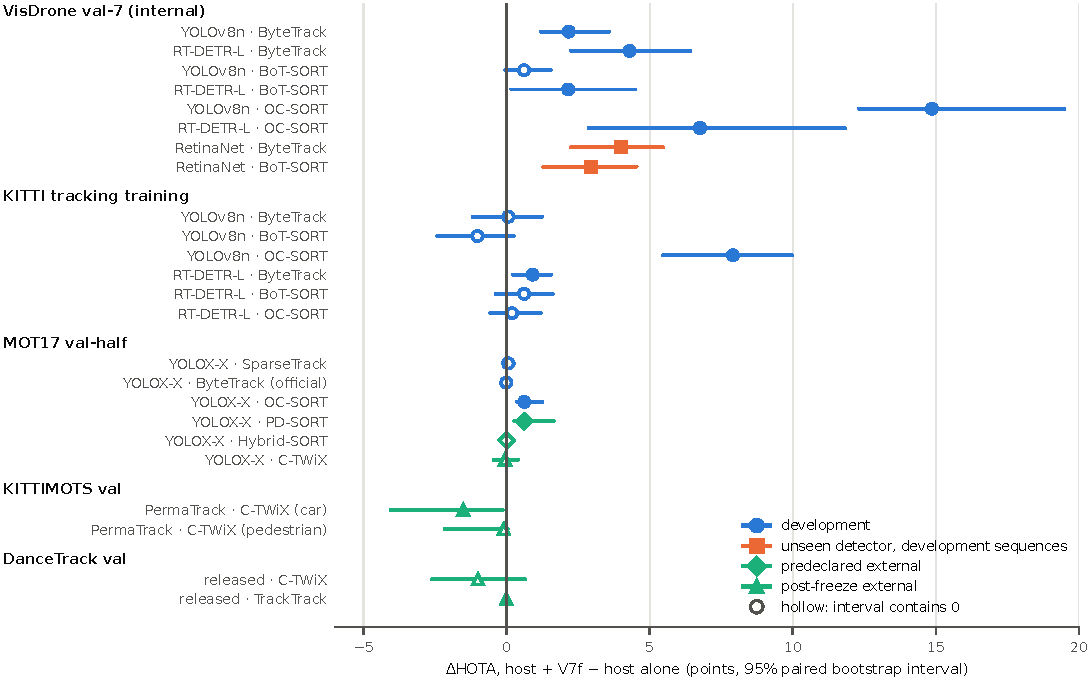
\includegraphics[width=0.92\textwidth]{figures/fig5_forest.pdf}
\caption{HOTA difference (host with the frozen layer minus host alone) with 95\% paired bootstrap intervals for every recorded combination, grouped by dataset and marked by evidence status. Filled markers: interval excludes zero. VisDrone rows use the frozen General AC-MOT configuration (V7f at 736 px); KITTI values are KITTI HOTA (car/pedestrian mean).}
\label{fig:forest}
\end{figure*}

\subsection{Transfer across trackers}\label{sec:tracker_transfer}
\paragraph{Predeclared external trackers.} Two published trackers were declared in the freeze commit of V7f and run once on MOT17 val-half with the YOLOX-X detections released by the PD-SORT authors. Our reproduction of PD-SORT~\cite{wang2025pdsort} matched the authors' released output to three decimals (\V{ext.pd.base.HOTA} HOTA). The frozen layer raised its HOTA by \Vz{ext.pd.dHOTA}, MOTA by \Vz{ext.pd.dMOTA} and IDF1 by \Vz{ext.pd.dIDF1}, while false negatives changed by \V{ext.pd.dFN} and false positives by \V{ext.pd.dFP}. PD-SORT is single-stage; Hybrid-SORT~\cite{yang2024hybridsort}, a two-stage host, produced identical output with and without the layer.

\paragraph{Post-freeze external trackers.} Three further systems were selected after the freeze under a written protocol that classified each reproduction before the layer was added. C-TWiX~\cite{miah2025twix} (coordinate-only association) changed by \Vz{ctx.mot.dHOTA} on MOT17, \Vz{ctx.kcar.dHOTA} on KITTIMOTS cars, \Vz{ctx.kped.dHOTA} on KITTIMOTS pedestrians and \Vz{ctx.dance.dHOTA} on DanceTrack. TrackTrack~\cite{shim2025tracktrack} (two detection views) changed by \Vz{tt.dance.dHOTA} on DanceTrack, an interval that excludes zero but a difference of about one hundredth of a point. TOPICTrack~\cite{cao2025topictrack} could not be reproduced within the protocol's tolerance (\V{tp.mot.base.HOTA} against \V{tp.mot.refHOTA} HOTA) and is excluded from the main results.

\paragraph{Development trackers behind the host contract on aerial data.} BoT-SORT and OC-SORT were development trackers of V7f; their VisDrone runs test whether the same frozen configuration works behind other host contracts on aerial data, not transfer to unseen trackers. With BoT-SORT, HOTA changed by \Vz{bot.yolov8.int.dHOTA} for YOLOv8n and \Vz{bot.rtdetr.int.dHOTA} for RT-DETR-L. With OC-SORT, whose fixed threshold left a recall of only \V{oc.yolov8.base.Recall}\% with YOLOv8n, HOTA rose by \Vz{oc.yolov8.int.dHOTA} and \Vz{oc.rtdetr.int.dHOTA}.

\begin{figure*}[t]
\centering
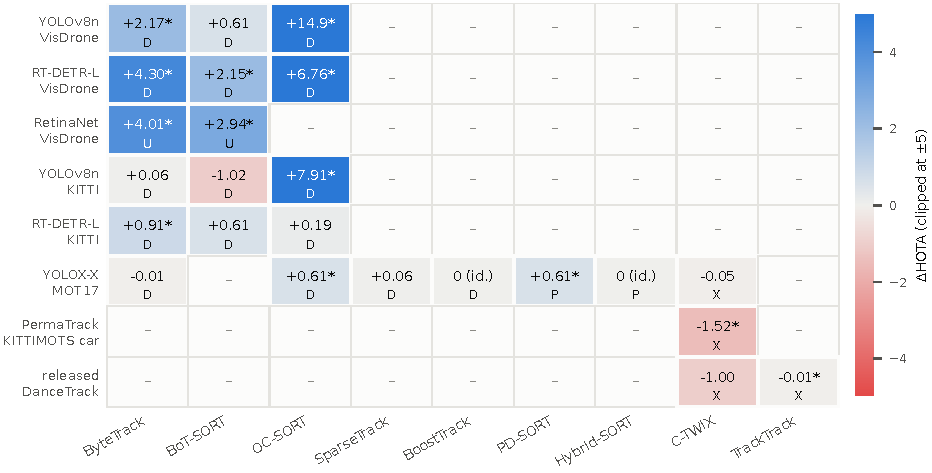
\includegraphics[width=\textwidth]{figures/fig6_transfer_matrix.pdf}
\caption{Transfer matrix: HOTA difference for each detector stream (rows) and tracker (columns); dashes mark combinations not run. Letters give the evidence status (D development, U unseen detector on development sequences, P predeclared external, X post-freeze external); an asterisk marks an interval that excludes zero; ``id.'' marks identical output.}
\label{fig:matrix}
\end{figure*}

\subsection{Transfer to an unseen detector}\label{sec:detector_transfer}
RetinaNet ResNet50-FPN v2~\cite{lin2017focal}, a one-stage detector with sigmoid focal-loss scores, entered the project only after the freeze of V7f; its adapter was added for General AC-MOT, and its transfer lock, which fixes the detector weights, the adapter, the hosts, the arms and two predictions (non-negative HOTA change with ByteTrack, no new catastrophic sequence), was committed before any RetinaNet tracking metric existed. Only the adapter (API translation) is new. The evaluation used the VisDrone val sequences, which are development sequences of V7f. With ByteTrack, General AC-MOT raised HOTA by \Vz{rn.by.736.int.dHOTA} under the internal protocol and \Vz{rn.by.736.off.dHOTA} under the official-compatible one; with BoT-SORT by \Vz{bot.retinanet.int.dHOTA} and \Vz{bot.retinanet.off.dHOTA} (Table~\ref{tab:retinanet}). Both predictions held. In the pre-declared compute arms the gain was smaller at 640 px (\Vz{rn.by.640.int.dHOTA}) and \Vz{rn.by.832.int.dHOTA} at 832 px. FCOS, chosen later as an unseen detector for a separate compute study, has not been evaluated.

\begin{table*}[!htbp]
\centering
\caption{Unseen detector: RetinaNet ResNet50-FPN v2 with the frozen General AC-MOT configuration, VisDrone2019-MOT val. The transfer lock (\texttt{research/TRANSFER\_LOCK\_RETINANET\_G1.json}) was committed before any RetinaNet tracking metric existed; only the detector adapter is new. The sequences are development sequences of V7f. Rows at 640 and 832 px are the pre-declared compute-curve arms. $\Delta$ = General AC-MOT $-$ host alone; +/$-$ counts sequences with higher/lower HOTA.}
\label{tab:retinanet}
\footnotesize
\setlength\tabcolsep{3.5pt}
\begin{tabular}{llcllllc}
\toprule
Host & Protocol & px & $\Delta$HOTA [95\% CI] & $\Delta$MOTA & $\Delta$IDF1 & $\Delta$IDS & +/$-$ \\
\midrule
ByteTrack & internal & 736 & +4.01 [+2.25, +5.46] & +9.12 [+0.80, +22.02] & +5.81 [+2.96, +7.99] & \textminus{}158 & 6/1 \\
ByteTrack & official-compatible & 736 & +4.84 [+3.37, +6.11] & +7.73 [+0.58, +17.40] & +6.08 [+3.99, +7.45] & \textminus{}824 & 7/0 \\
BoT-SORT & internal & 736 & +2.94 [+1.28, +4.54] & +11.00 [+1.78, +24.77] & +4.55 [+1.78, +6.82] & \textminus{}86 & 6/1 \\
BoT-SORT & official-compatible & 736 & +4.22 [+2.98, +5.30] & +9.56 [+1.44, +19.79] & +5.59 [+3.63, +7.07] & \textminus{}959 & 7/0 \\
ByteTrack & internal & 640 & +0.89 [\textminus{}0.24, +2.24] & +8.53 [+3.56, +15.54] & +1.28 [\textminus{}0.09, +3.35] & \textminus{}45 & 2/5 \\
ByteTrack & official-compatible & 640 & +1.92 [+0.62, +3.54] & +7.74 [+2.52, +14.62] & +2.30 [+0.78, +4.54] & \textminus{}670 & 6/1 \\
ByteTrack & internal & 832 & +3.62 [+1.94, +5.14] & +10.81 [+3.82, +21.88] & +4.60 [+2.23, +6.50] & \textminus{}171 & 6/1 \\
ByteTrack & official-compatible & 832 & +3.97 [+2.29, +5.74] & +9.68 [+3.53, +18.17] & +5.06 [+3.22, +6.98] & \textminus{}892 & 7/0 \\
\botrule
\end{tabular}
\end{table*}


\subsection{Transfer to other datasets}\label{sec:dataset_transfer}
The external systems add two settings beyond the development data: KITTIMOTS val with PermaTrack detections~\cite{tokmakov2021permatrack} (a new detector on sequences that are part of the KITTI training split used in development) and DanceTrack val, the only dataset that no development run used. On DanceTrack the layer changed C-TWiX by \Vz{ctx.dance.dHOTA} and TrackTrack by \Vz{tt.dance.dHOTA}: neither a gain nor a large loss. On KITTIMOTS the C-TWiX car result is the one significant external degradation (\Vz{ctx.kcar.dHOTA}), analysed in Sect.~\ref{sec:boundary}. The frozen layer was not evaluated on UAVDT, VisDrone test-dev or the reserved VisDrone confirmation split.

\subsection{Robustness to detector-score calibration shift}\label{sec:calib}
Table~\ref{tab:calib} applies four monotone score transformations to the MOT17 development streams before the tracker. Of \V{cal.n} host--transformation conditions, \V{cal.rec} showed significant recoveries, \V{cal.deg} significant degradations, \V{cal.ident} identical outputs and \V{cal.ns} no significant change. The halved scale that drove ByteTrack (official) and OC-SORT to zero was restored to \V{cal.byoff.scale05.v7f} and \V{cal.oc.scale05.v7f} HOTA. The library ByteTrack under a temperature of~2 was not corrected (identical output): its clean-regime thresholds are only lowered, never raised. These are development hosts, so the intervals quantify robustness, not held-out generalization.

\begin{tableorg}[!htbp]
\centering
\caption{Detector-score calibration shift on MOT17 val-half (published YOLOX-X detections, development hosts). The detector scores are transformed before the tracker; the frozen V7f layer is not changed. HOTA of the host alone and with V7f; paired sequence bootstrap, 10,000 resamples, seed 42. 14 conditions: 7 significant recoveries, 0 significant degradations, 2 identical outputs.}
\label{tab:calib}
\footnotesize
\setlength\tabcolsep{3.5pt}
\begin{adjustbox}{max width=\linewidth}
\begin{tabular}{llrrlcl}
\toprule
Host & Transform & Host alone & + V7f & $\Delta$HOTA [95\% CI] & W/T/L & Verdict \\
\midrule
ByteTrack (official setting) & $s^3$ & 60.92 & 65.81 & +4.89 [+2.60, +13.69] & 7/0/0 & significant recovery \\
ByteTrack (official setting) & $0.5\,s$ & 0.00 & 66.17 & +66.17 [+49.32, +75.40] & 7/0/0 & significant recovery \\
ByteTrack (official setting) & logit $/2$ & 65.84 & 66.95 & +1.11 [+0.35, +3.87] & 6/0/1 & significant recovery \\
ByteTrack (official setting) & logit $\times 2$ & 67.30 & 67.29 & \ensuremath{-}0.01 [\ensuremath{-}0.05, 0.00] & 1/4/2 & no significant change \\
ByteTrack (library default) & $s^3$ & 66.31 & 66.31 & \ensuremath{-}0.01 [\ensuremath{-}0.38, +0.38] & 3/0/4 & no significant change \\
ByteTrack (library default) & $0.5\,s$ & 66.61 & 66.48 & \ensuremath{-}0.14 [\ensuremath{-}0.66, +0.14] & 2/3/2 & no significant change \\
ByteTrack (library default) & logit $/2$ & 63.97 & 63.97 & 0.00 [0.00, 0.00] & 0/7/0 & identical output \\
ByteTrack (library default) & logit $\times 2$ & 66.53 & 66.52 & \ensuremath{-}0.01 [\ensuremath{-}0.03, 0.00] & 0/5/2 & no significant change \\
OC-SORT & $s^3$ & 58.34 & 66.60 & +8.26 [+5.86, +16.81] & 7/0/0 & significant recovery \\
OC-SORT & $0.5\,s$ & 0.00 & 66.72 & +66.72 [+50.32, +75.56] & 7/0/0 & significant recovery \\
OC-SORT & logit $/2$ & 65.99 & 67.22 & +1.24 [+0.52, +3.42] & 6/0/1 & significant recovery \\
OC-SORT & logit $\times 2$ & 66.61 & 67.06 & +0.45 [\ensuremath{-}0.01, +0.97] & 4/0/3 & no significant change \\
BoostTrack (online) & $s^3$ & 61.33 & 64.84 & +3.51 [+0.85, +13.28] & 7/0/0 & significant recovery \\
BoostTrack (online) & logit $/2$ & 67.59 & 67.59 & 0.00 [0.00, 0.00] & 0/7/0 & identical output \\
\botrule
\end{tabular}
\end{adjustbox}
\end{tableorg}


%==========================================================================================
\section{Ablation}\label{sec:ablation}
%==========================================================================================
\paragraph{From native host to full V7f.} Table~\ref{tab:ablation} adds one mechanism at a time on MOT17 development hosts. The pass-through path (adapters and layer without intervention) reproduced the hosts exactly on \V{abl.passthrough.identical} of \V{abl.passthrough.cells} host/floor cells, and its SparseTrack and BoostTrack outputs were byte-identical to the official replays. Self-calibration alone, applying the nested-Otsu bands to every frame, reduced ByteTrack (official) from \V{abl.host.by} to \V{abl.v6.by} and OC-SORT from \V{abl.host.oc} to \V{abl.v6.oc}. The host-aware regime with a clean regime anchored to the host and crowd-safe duplicates recovered most of the loss; estimating the regime from the whole stream, the track continuation and the interpretability check brought ByteTrack and BoostTrack back to their host-alone values and OC-SORT above its host alone (\V{abl.v7f.oc} against \V{abl.host.oc}). On KITTI with YOLOv8n and OC-SORT the continuation stage contributed most (\V{abl.v7d.kitoc} to \V{abl.v7e.kitoc}). These are development values without intervals.

\begin{table*}[!htbp]
\centering
\caption{Mechanism ablation, one change at a time (HOTA). MOT17 val-half with published YOLOX-X detections at the 0.1 score floor, no image motion cue.}
\label{tab:ablation}
\footnotesize
\setlength\tabcolsep{3.5pt}
\begin{tabular}{p{7.2cm}rrrr}
\toprule
Variant & ByteTrack (official) & OC-SORT & BoostTrack & KITTI OC-SORT \\
\midrule
Native host through the layer and adapters, no intervention (pass-through) & 67.70 & 66.44 & 68.49 & -- \\
Self-calibration only: nested-Otsu bands always applied, IoU duplicate rule, rank scores (prior design) & 56.41 & 45.72 & 62.55 & 40.20 \\
+ host-aware regime ($\rho$ over 100 frames), clean regime anchored to the host, crowd-safe duplicates & 67.56 & 65.70 & 68.37 & 41.13 \\
+ regime estimated from the whole stream & 67.70 & 66.07 & 68.47 & -- \\
+ foreground track-consistent continuation & 67.70 & 66.47 & 68.47 & 44.15 \\
+ interpretability check of the split = frozen V7f & 67.70 & 66.91 & 68.49 & 44.17 \\
Host alone (original driver) & 67.70 & 66.44 & 68.49 & 36.27 \\
\botrule
\end{tabular}
\par\smallskip\parbox{\linewidth}{\scriptsize Pass-through: on 7 of 7 MOT17 host/floor cells the pass-through output equals the host alone in every metric, and the SparseTrack and BoostTrack pass-through track files are byte-identical to the official replays (development ledger, E0). KITTI column: YOLOv8n + OC-SORT, KITTI HOTA. All rows are development evidence; no interval is claimed.}
\end{table*}


\paragraph{Rejected alternatives.} Variants recorded in the development ledger were not adopted: starting without host thresholds in cold frames, continuing tracks from candidates below the host's lowest stage, remapping scores in clean frames, projecting the host operating point onto the noisy bands, and pooling scores before duplicate handling. On the development hosts they lowered HOTA, left it unchanged, or, for the projection, passed many more boxes per frame on a noisy stream.

\paragraph{Scene control on top of V7f.} A pre-registered factorial on VisDrone val (Table~\ref{tab:factorial}) combined the historical SCI resolution rule with V7f. V7f alone gained \Vz{fw.c_a.int.dHOTA} HOTA over the native host; the SCI alone changed HOTA by \Vz{fw.b_a.int.dHOTA}; adding the SCI on top of V7f changed it by \Vz{fw.d_c.int.dHOTA} and, under the official-compatible protocol, lowered MOTA by \Vz{fw.d_c.off.dMOTA}; and the SCI schedule was indistinguishable from budget-matched shuffled schedules. Static compute points behaved as expected: relative to 736 px, 832 px changed HOTA by \Vz{fw.high.int.dHOTA} and 640 px by \Vz{fw.low.int.dHOTA}. The score layer and the compute decision can be composed without changing V7f, but the historical scene rule added neither accuracy nor a compute saving.

\begin{tableorg}[!htbp]
\centering
\caption{Pre-registered factorial on VisDrone2019-MOT val (ByteTrack, YOLOv8n and RT-DETR-L, pooled over 14 detector--sequence cells). The historical scene controller is compared with and without V7f, and with budget-matched scene-blind schedules. Paired bootstrap, 10,000 resamples, seed 42.}
\label{tab:factorial}
\footnotesize
\setlength\tabcolsep{3.5pt}
\begin{adjustbox}{max width=\linewidth}
\begin{tabular}{p{5.6cm}llll}
\toprule
Comparison & $\Delta$HOTA internal & $\Delta$MOTA internal & $\Delta$HOTA official & $\Delta$MOTA official \\
\midrule
V7f only $-$ native (C$-$A) & +2.98 [+1.76, +4.47] & +14.17 & +2.29 [+1.19, +3.59] & +11.59 [+4.15, +21.16] \\
historical SCI only $-$ native (B$-$A) & \ensuremath{-}0.21 [\ensuremath{-}0.45, \ensuremath{-}0.01] & \ensuremath{-}0.31 & \ensuremath{-}0.17 [\ensuremath{-}0.42, +0.01] & \ensuremath{-}0.29 [\ensuremath{-}0.89, +0.28] \\
SCI + V7f $-$ V7f only (D$-$C) & \ensuremath{-}0.17 [\ensuremath{-}0.56, +0.20] & \ensuremath{-}0.18 & \ensuremath{-}0.26 [\ensuremath{-}0.59, +0.04] & \ensuremath{-}0.77 [\ensuremath{-}1.51, \ensuremath{-}0.20] \\
SCI + V7f $-$ SCI only (D$-$B) & +3.03 [+1.73, +4.62] & +14.30 & +2.20 [+1.06, +3.57] & +11.11 [+3.55, +20.91] \\
SCI + V7f $-$ budget-matched shuffled schedule, seed 1 & \ensuremath{-}0.03 [\ensuremath{-}0.30, +0.24] & \ensuremath{-}0.09 & \ensuremath{-}0.07 [\ensuremath{-}0.27, +0.14] & \ensuremath{-}0.34 [\ensuremath{-}1.05, +0.21] \\
SCI + V7f $-$ shuffled schedule, seed 2 & +0.04 [\ensuremath{-}0.25, +0.33] & \ensuremath{-}0.12 & \ensuremath{-}0.19 [\ensuremath{-}0.48, +0.07] & \ensuremath{-}0.60 [\ensuremath{-}1.17, \ensuremath{-}0.15] \\
SCI + V7f $-$ shuffled schedule, seed 3 & +0.05 [\ensuremath{-}0.32, +0.48] & \ensuremath{-}0.02 & \ensuremath{-}0.18 [\ensuremath{-}0.47, +0.15] & \ensuremath{-}0.37 [\ensuremath{-}0.87, +0.11] \\
V7f at 832 px $-$ V7f at 736 px & +0.74 [+0.05, +1.48] & +1.16 & +0.96 [+0.60, +1.42] & +0.59 [\ensuremath{-}0.88, +2.12] \\
V7f at 640 px $-$ V7f at 736 px & \ensuremath{-}1.22 [\ensuremath{-}1.89, \ensuremath{-}0.55] & \ensuremath{-}1.69 & \ensuremath{-}1.27 [\ensuremath{-}1.80, \ensuremath{-}0.82] & \ensuremath{-}1.87 [\ensuremath{-}3.40, \ensuremath{-}0.60] \\
\botrule
\end{tabular}
\end{adjustbox}
\par\smallskip\parbox{\linewidth}{\scriptsize Relative compute of the scene-adaptive arms: SCI only 0.949 (YOLOv8n) / 1.026 (RT-DETR-L); SCI + V7f 0.979 / 1.012; 832 px 1.278; 640 px 0.756 (736 px = 1). The decision rule was committed before the first result.}
\end{tableorg}


%==========================================================================================
\section{Runtime Analysis}\label{sec:runtime}
%==========================================================================================
Table~\ref{tab:runtime} and Fig.~\ref{fig:runtime} report CPU timings. With live YOLOv8n and ByteTrack on KITTI frames (\V{rt.cpu}, \V{rt.threads} threads), the layer took \V{rt.v7f.ctrl}~ms per frame on average (P95 \V{rt.v7f.ctrl95}~ms), and end-to-end time rose by \V{rt.e2e_delta}~ms (\V{rt.e2e_pct}\% including frame reading, \V{rt.pipe_pct}\% excluding it). On a two-thread \V{g1rt.cpu} runner with VisDrone frames, the layer, including its motion cue, took \V{g1rt.yolov8.g1.score}, \V{g1rt.rtdetr.g1.score} and \V{g1rt.retinanet.g1.score}~ms with YOLOv8n, RT-DETR-L and RetinaNet, an overhead of \V{g1rt.yolov8.pct}\%, \V{g1rt.rtdetr.pct}\% and \V{g1rt.retinanet.pct}\% of the total. The tracker became faster with the layer because fewer candidates reached it. None of these CPU pipelines runs at video rate, and no GPU timing of V7f was available; we do not convert CPU throughput to other hardware. For Stage 1, the cue analysis of the adaptive controller was not profiled separately; in the matched static configuration on the T4, the detector took \V{t4.det}~ms and the tracker \V{t4.trk}~ms per frame.

\begin{tableorg}[!htbp]
\centering
\caption{Runtime per frame (ms). Mean unless marked P95.}
\label{tab:runtime}
\footnotesize
\setlength\tabcolsep{3.5pt}
\begin{adjustbox}{max width=\linewidth}
\begin{tabular}{p{3.6cm}rlrrrrl}
\toprule
Configuration & Detector & Control layer & Tracker & Total & P95 total & FPS & Overhead \\
\midrule
\multicolumn{8}{l}{\textit{V7f layer, YOLOv8n + ByteTrack, KITTI frames, Intel Xeon @ 2.10 GHz, 4 vCPU (4 threads), 736 px, 2,279 frames per arm}} \\
Host alone & 41.91 & 0.02 & 2.04 & 57.85 & 76.35 & 17.29 & -- \\
+ V7f & 42.17 & 2.95 (P95 4.39) & 1.43 & 60.44 & 80.78 & 16.55 & +2.59 ms (+4.5\%) \\
\midrule
\multicolumn{8}{l}{\textit{General AC-MOT, VisDrone val frames, AMD EPYC 7763 (2 threads), 736 px, 300 frames, decode excluded}} \\
YOLOv8n, host alone & 83.35 & 0.03 & 3.27 & 86.66 & 90.19 & 11.540 & -- \\
YOLOv8n, General AC-MOT & 84.82 & 5.23 & 2.76 & 92.82 & 96.06 & 10.774 & +7.1\% \\
RT-DETR-L, host alone & 1196.51 & 0.05 & 7.61 & 1204.17 & 1273.61 & 0.830 & -- \\
RT-DETR-L, General AC-MOT & 1213.04 & 7.38 & 3.64 & 1224.07 & 1293.81 & 0.817 & +1.7\% \\
RetinaNet, host alone & 935.50 & 0.07 & 6.11 & 941.69 & 950.11 & 1.062 & -- \\
RetinaNet, General AC-MOT & 934.16 & 13.14 & 4.97 & 952.27 & 971.14 & 1.050 & +1.1\% \\
\botrule
\end{tabular}
\end{adjustbox}
\par\smallskip\parbox{\linewidth}{\scriptsize End-to-end time in the first block includes frame reading; the overhead relative to the pipeline without reading is +5.9\%. The control-layer time includes its quarter-resolution phase-correlation motion cue. The tracker is faster with the layer because fewer candidates reach it. CPU measurements only; no GPU timing of V7f or General AC-MOT was available, and no FPS is converted to other hardware.}
\end{tableorg}


\begin{figure}[t]
\centering
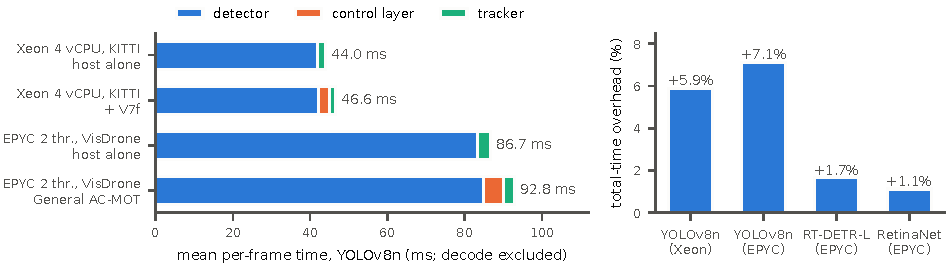
\includegraphics[width=\linewidth]{figures/fig7_runtime.pdf}
\caption{Runtime. Left: mean per-frame time of detector, control layer and tracker with YOLOv8n, host alone and with the layer, on two CPUs (decode excluded). Right: total-time overhead of the layer for three detectors. CPU measurements only.}
\label{fig:runtime}
\end{figure}

%==========================================================================================
\section{Comparison with Published Methods}\label{sec:published}
%==========================================================================================
Table~\ref{tab:published} compares, for each published tracker, the number reported by its authors, our reproduction, and the reproduction with the frozen layer. The comparison is fair only in one sense: the layer is added to the same reproduced system on the same split with the same evaluator, so the difference measures what the layer contributes. The included reproductions differ from the reported values by less than one HOTA point (TOPICTrack failed the reproduction criterion and is excluded), the reported values are validation-split numbers, and none of our numbers is a test-server result. We therefore make no claim of state-of-the-art accuracy and do not rank our system against the published trackers. On VisDrone and UAVDT, published tracker results are usually reported with the official toolkits, on other splits or with other detectors; our Stage-1 protocol is custom and the official-compatible port is not the evaluation server, so those results are not directly comparable and are not tabulated against published numbers.

\begin{tableorg}[!htbp]
\centering
\caption{Published trackers: number reported by the authors, our reproduction (host alone), and the reproduction with the frozen V7f layer (HOTA; reported number as HOTA / MOTA / IDF1 where available). The comparison measures what the layer adds to each published system, not a ranking between systems.}
\label{tab:published}
\footnotesize
\setlength\tabcolsep{3.5pt}
\begin{adjustbox}{max width=\linewidth}
\begin{tabular}{p{3.8cm}p{4.2cm}rrlc}
\toprule
System & Reported & Reproduction & + V7f & $\Delta$HOTA [95\% CI] & St. \\
\midrule
SparseTrack (TCSVT 2025) & 69.2 / 76.8 / 81.4 (paper, val) & 68.876 & 68.931 & +0.055 [\ensuremath{-}0.011, +0.254] & D \\
BoostTrack (MVA 2024), online & 68.371 / 75.561 / 81.354 (authors' corrected) & 68.492 & 68.492 & 0 (identical) & D \\
ByteTrack (ECCV 2022) & -- / 76.6 / 79.3 (own detector run) & 67.698 & 67.684 & \ensuremath{-}0.014 [\ensuremath{-}0.058, +0.009] & D \\
OC-SORT (CVPR 2023) & 66.5 / 74.9 / 77.7 (paper, val-half) & 66.428 & 67.041 & +0.613 [+0.363, +1.241] & D \\
PD-SORT (TCE 2025) & 68.011 (authors' released output) & 68.011 & 68.624 & +0.613 [+0.268, +1.646] & P \\
Hybrid-SORT (AAAI 2024) & 67.1 / 75.8 / 78.0 (README) & 66.698 & 66.698 & 0 (identical) & P \\
C-TWiX (PR 2025), MOT17 & 77.8 (README) & 77.550 & 77.495 & \ensuremath{-}0.055 [\ensuremath{-}0.456, +0.398] & X \\
C-TWiX, KITTIMOTS car & 89.3 (README) & 89.266 & 87.745 & \ensuremath{-}1.521 [\ensuremath{-}4.053, \ensuremath{-}0.134] & X \\
C-TWiX, DanceTrack & 60.4 (README) & 59.615 & 58.610 & \ensuremath{-}1.005 [\ensuremath{-}2.622, +0.646] & X \\
TrackTrack (CVPR 2025), DanceTrack & 63.3 (paper, post-processed) & 62.961 & 62.948 & \ensuremath{-}0.013 [\ensuremath{-}0.032, \ensuremath{-}0.001] & X \\
TOPICTrack (TIP 2025), MOT17 & 69.6 (paper) & 67.538 & -- & reproduction failed; excluded & X \\
\botrule
\end{tabular}
\end{adjustbox}
\par\smallskip\parbox{\linewidth}{\footnotesize All values are validation-split evaluations with TrackEval in our environment, on the same split the published number refers to; none is a test-server number, and none is comparable with leaderboard results. VisDrone and UAVDT results in this paper use a custom or official-compatible protocol that differs from the published VisDrone/UAVDT benchmarks; they are not directly comparable with published tracker numbers on those benchmarks and are not compared here.}
\end{tableorg}


The contribution claimed here is therefore not a higher HOTA than any published tracker. It is a training-free, causal layer that needs no target-specific calibration, separates the policy from detector and tracker through adapters and a host contract, self-calibrates scores online, is deployed as one frozen policy, transfers across the tested systems with low overhead, and comes with a reproducibility record.

%==========================================================================================
\section{Generalization Analysis and Boundary Cases}\label{sec:boundary}
%==========================================================================================
\paragraph{Where the layer helps.} The gains concentrate in three situations: trackers without a low-score stage whose fixed threshold does not fit the detector (OC-SORT on MOT17, on KITTI with YOLOv8n, and on VisDrone; PD-SORT), noisy or miscalibrated detector streams (RT-DETR-L and RetinaNet on VisDrone, RT-DETR-L on KITTI), and shifted score scales (Table~\ref{tab:calib}). On two-stage trackers with well-matched detections the layer is transparent or nearly so.

\paragraph{Trade-offs between metrics.} Gains in HOTA and IDF1 are not always gains in MOTA or recall. With RT-DETR-L on VisDrone, false positives changed by \V{vd.rtdetr.int.dFP} and false negatives by \V{vd.rtdetr.int.dFN}; recall fell from \V{vd.rtdetr.base.int.Recall} to \V{vd.rtdetr.g1.int.Recall}. With OC-SORT, false positives rose (\V{oc.yolov8.base.FP} to \V{oc.yolov8.g1.FP} for YOLOv8n) as recall rose. With PD-SORT, false positives changed by \V{ext.pd.dFP} and false negatives by \V{ext.pd.dFN}.

\paragraph{A tracker without enough evidence: C-TWiX on KITTIMOTS cars.} The one significant external degradation (\Vz{ctx.kcar.dHOTA}) came from a sparse stream: the regime statistic of sequence 0014 stayed between \V{fig8.rhomin} and \V{fig8.rhomax} after its first 50 frames, the regime switched \V{fig8.switches} times and \V{fig8.noisy} of its \V{fig8.frames} frames were judged noisy (Fig.~\ref{fig:boundary}, left); the car HOTA of that sequence changed by \V{ctx.kcar.seq0014}. A regime decision without a margin or hysteresis is fragile when few candidates per frame are available. On DanceTrack, C-TWiX changed by \Vz{ctx.dance.dHOTA}; which operation caused this was not isolated.

\paragraph{An under-confident detector with two-stage trackers.} With YOLOv8n on KITTI, the noisy-regime birth restriction cost ByteTrack and BoT-SORT MOTA (\V{kitd.yolov8.by.dMOTA}, \V{kitd.yolov8.bot.dMOTA}) while identity switches changed by \V{kitd.yolov8.by.dIDS} and \V{kitd.yolov8.bot.dIDS}; the BoT-SORT HOTA interval contains zero.

\paragraph{New catastrophic sequences.} Under the official-compatible protocol, General AC-MOT with OC-SORT produced \V{oc.cat.g1.off} catastrophic sequences where OC-SORT alone had \V{oc.cat.base.off}, although HOTA rose on both detectors; the cause of this trade-off was not isolated.

\paragraph{No headroom for dynamic compute.} The compute interface of General AC-MOT is constant because adaptive compute did not pay off on the tested aerial data. Beyond the factorial of Sect.~\ref{sec:ablation}, a ground-truth oracle that allocates 640, 736 or 832 px per 30-frame segment at the compute of a fixed 736 px gained only \Vz{or.m3} HOTA, and an oracle over nine resolutions \Vz{or.f736}; no causal cue met the selection rule declared for the cue audit. Compute itself paid off in a detector-specific way (Fig.~\ref{fig:boundary}, right): from 512 to 960 px, HOTA with V7f rose much more for YOLOv8n than for RT-DETR-L. In a supplementary study of compute allocation, pre-registered oracle gates (an oracle gain of at least \V{g2.gate} HOTA with an interval above zero, or the same HOTA at no more than \V{g2.cost} of the cost) were not met for resolution allocation (best \Vz{g2.s1_100}) or for invocation frequency combined with resolution (best \Vz{g2.s2_35}). A scene-response index from that study, fitted and scored on the same development segments, ranked segment difficulty (mean rank correlation \V{gsci.D.G}) but did not locate where extra compute pays off (\V{gsci.B.G}); it is a difficulty measure, not a compute controller. That study is not part of the method, and its tile-refinement stage was not complete when this paper was written.

\begin{figure*}[t]
\centering
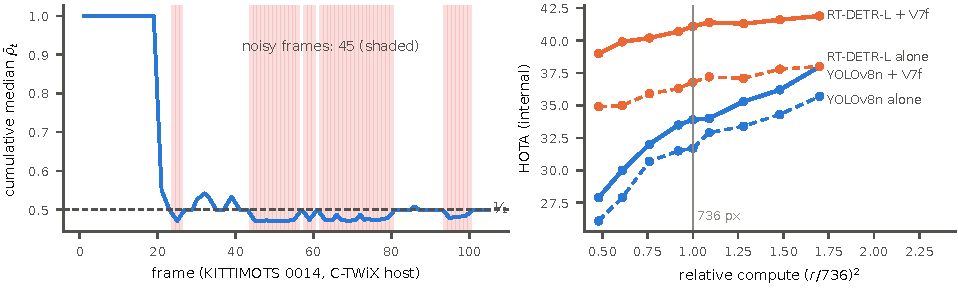
\includegraphics[width=\textwidth]{figures/fig8_boundary.pdf}
\caption{Boundary cases. Left: cumulative median regime statistic $\bar\rho_t$ of C-TWiX on KITTIMOTS sequence 0014 (frozen V7f audit log); shaded frames were judged noisy; $\bar\rho_t$ hovers around the boundary $\frac12$. Right: HOTA with and without V7f against relative detector compute on VisDrone val (ByteTrack, internal protocol; values from the development record, no intervals); the benefit of compute differs strongly between detectors.}
\label{fig:boundary}
\end{figure*}

%==========================================================================================
\section{Discussion}\label{sec:discussion}
%==========================================================================================
\paragraph{One idea, two placements.} AC-MOT and General AC-MOT apply the same idea, operating-point control, at two places. Before the detector, the controller could find a good operating point for one detector and one tracker, and that operating point carried its gain. Behind the detector, the layer can see what a controller before the detector cannot: the scale and separation of the detector's own scores. Moving the control point there turned a calibration that had to be redone for every pipeline into one that is redone online, by the layer, for every stream.

\paragraph{Restraint as part of adaptation.} The step from the always-on predecessor to V7f was not more adaptation but adaptation with restraint: estimating whether the tracker's declared operating point already fits, and doing nothing when it does. The ablation shows that this restraint is what keeps strong two-stage trackers unchanged, while the continuation stage and the noisy-regime bands supply what single-stage trackers and noisy detectors lack.

\paragraph{What the evidence supports.} The development evidence is broad (two detectors run by us and published YOLOX-X detections, five trackers, three datasets), but it is development evidence. The external evidence is narrower: one significant improvement of a predeclared tracker, one transparent predeclared tracker, mixed post-freeze results with one significant loss, and one unseen detector on development sequences. The appropriate claim is that one frozen policy transfers across the heterogeneous detection--tracking pipelines we tested, helps where the tracker's operating point does not fit the stream, and stays out of the way of most well-matched trackers, not that it improves every tracker.

%==========================================================================================
\section{Limitations}\label{sec:limits}
%==========================================================================================
\begin{enumerate}
\item \emph{Development versus external evidence.} Most positive V7f results are on development data or hosts. External evidence covers two predeclared and three post-freeze trackers, mostly on MOT17 val-half, and one unseen detector evaluated on development sequences.
\item \emph{No test-server or official benchmark results.} All MOT17, KITTI and DanceTrack values are validation-split evaluations; VisDrone results use a custom or an official-compatible protocol.
\item \emph{No held-out aerial result for V7f.} The frozen layer was not evaluated on VisDrone test-dev, UAVDT or the reserved VisDrone confirmation split.
\item \emph{Hardware.} V7f and General AC-MOT were timed on CPUs only; Stage-1 timing excludes frame decoding and varied between sessions.
\item \emph{Regime decision.} The boundary $\bar\rho_t\ge\frac12$ has no margin or hysteresis, which caused the significant C-TWiX loss; the clean regime never raises thresholds, so a host whose thresholds are too low for a stream is not corrected.
\item \emph{Design constants.} The regime boundary and the mechanism choices were fixed on labelled development data; they are not fitted at deployment but were not derived without labels.
\item \emph{Untested parts.} The motion rule was inactive in every MOT17 and external experiment; no head-to-head comparison with trackers that adapt their own thresholds per frame was run.
\item \emph{Statistical resolution.} Intervals are per comparison, without correction for multiple comparisons, and with seven VisDrone validation sequences differences below about half a HOTA point are not resolvable.
\item \emph{Stage-1 scope.} Stage 1 used one detector and one tracker profile; its matched-static attribution is post hoc and its per-sequence values were not archived.
\end{enumerate}

%==========================================================================================
\section{Conclusion}\label{sec:conclusion}
%==========================================================================================
AC-MOT began as scene adaptation, and it worked. Analysing why it worked showed that the generalizable part was not the scene index but operating-point calibration. Raw detector scores and scene indices did not carry that calibration across detectors and pipelines, so we turned it into a self-calibrating layer placed between the detector and the tracker, which separates the control logic from the scale of the detector's scores and from the properties of the tracker. One frozen policy, without training, without target-specific calibration and with a small runtime cost, improved an unseen detector and a predeclared external tracker, restored trackers whose input scores had been shifted, and left most well-matched trackers unchanged; it also failed in identifiable conditions, chiefly sparse streams near the regime boundary. A regime decision with a margin, held-out aerial and test-server evaluations, and GPU timing are the next steps.

\backmatter

\bmhead{Acknowledgements}
The authors thank the authors of the evaluated detectors and trackers for releasing their code, weights and detections, and the maintainers of VisDrone, UAVDT, MOT17, KITTI, DanceTrack and TrackEval.

\section*{Declarations}

\noindent\textbf{Funding:} The authors declare that no funds, grants, or other support were received during the preparation of this manuscript.

\noindent\textbf{Competing interests:} The authors have no relevant financial or non-financial interests to disclose.

\noindent\textbf{Ethics approval and consent to participate:} Not applicable.

\noindent\textbf{Consent for publication:} Not applicable.

\noindent\textbf{Data availability:} All datasets used (VisDrone2019-MOT, UAVDT, MOT17, KITTI tracking, DanceTrack) are publicly available from their providers. Tracker outputs, bootstrap records, derived detector caches with their SHA-256 checksums, the frozen configurations and their file-hash locks are available from the corresponding author on reasonable request.

\noindent\textbf{Materials availability:} Not applicable.

\noindent\textbf{Code availability:} The implementation of the controller and the layer, the adapters, the evaluation scripts and the scripts that regenerate every table, figure and number of this paper from the result records are available from the corresponding author on reasonable request. The frozen systems are identified by version tags (Stage~1: \texttt{v1.0.0-acmot-frozen}; V7f: \texttt{universal-acmot-v7-freeze}; General AC-MOT: \texttt{general-acmot-g1-freeze}).

\noindent\textbf{Author contribution:} Ahmed Gouda Ismail: conceptualization, methodology, software, experiments, formal analysis, writing of the original draft. Mohamed S. Mohamed and Tarek Ahmed Mahmoud: supervision, methodology review, writing (review and editing). All authors read and approved the final manuscript.

\bibliography{references}

\end{document}
